
\documentclass[oneside,12pt,french,table]{book}
\usepackage[french]{babel}
\usepackage[margin=1in]{geometry}
\usepackage{setspace} 
\setstretch{1.1}
% Lorem ipsum paragraphs
\usepackage{lipsum}

% Paragraph spacing
\usepackage{parskip}

% Custom fonts. This package is only available with XeLaTex (pdflatex is a mess to deal with)
\usepackage{fontspec}
\setmainfont{GeneralSans}[
    Path = assets/fonts/,
    Extension = .otf,
    UprightFont = *-Regular,
    ItalicFont = *-Italic,
    BoldFont = *-Bold,
    BoldItalicFont = *-BoldItalic
]

% Fancy chapters
\usepackage[Bjornstrup]{fncychap}
\ChTitleVar{\Large\flushright\bfseries}

% Mathematical packages
\usepackage{amsmath}
\usepackage{amsfonts}

% Theorem styling and environments
\usepackage{amsthm}
\theoremstyle{definition}
\newtheorem{definition}{Définition}[chapter]

\theoremstyle{plain}
\newtheorem{theorem}[definition]{Théorème}

\theoremstyle{remark}
\newtheorem{remark}[definition]{Remarque}

\theoremstyle{plain}
\newtheorem{lemma}[definition]{Lemme}

\theoremstyle{plain}
\newtheorem{proposition}[definition]{Proposition}

\theoremstyle{plain}
\newtheorem{corollary}[definition]{Corollaire}

% Boxed theorems
\usepackage{tcolorbox}

\newenvironment{greybox}{%
    \begin{tcolorbox}[boxrule=0pt, frame empty]
}{\end{tcolorbox}}

\newenvironment{boxdef}{
    \begin{tcolorbox}[boxrule=0pt, frame empty]
    \begin{definition}
}{
    \end{definition}
    \end{tcolorbox}
}

\newenvironment{boxthm}{
    \begin{tcolorbox}[boxrule=0pt, frame empty]
    \begin{theorem}
}{
    \end{theorem}
    \end{tcolorbox}
}

\newenvironment{boxlemma}{
    \begin{tcolorbox}[boxrule=0pt, frame empty]
    \begin{lemma}
}{
    \end{lemma}
    \end{tcolorbox}
}

\newenvironment{boxprop}{
    \begin{tcolorbox}[boxrule=0pt, frame empty]
    \begin{proposition}
}{
    \end{proposition}
    \end{tcolorbox}
}

\newenvironment{boxcor}{
    \begin{tcolorbox}[boxrule=0pt, frame empty]
    \begin{corollary}
}{
    \end{corollary}
    \end{tcolorbox}
}

% Graphics
\usepackage{tikz}
\usetikzlibrary{calc}
\usepackage{graphicx}
\usepackage{tkz-tab}
\usepackage{float} % for float positioning, in particular the H modifier
\usepackage{subcaption} % for subfigures and subcaptions
\usepackage{pgfplots}
\pgfplotsset{compat=newest}
%\pgfplotsset{%
%  every tick label/.append style = {font=\tiny},
%  every axis label/.append style = {font=\scriptsize}
%}

\tikzset{%
  point/.style = {fill=black,inner sep=1pt, circle, minimum width=3pt,align=right,rotate=60},
  } 
\tikzstyle{weight} = [font=\scriptsize]  
\tikzstyle{vertex}=[circle,fill=blue!20]

% Clickable links
\usepackage{xcolor} % table for colored tables
\definecolor{S4S-light}{HTML}{50527F}
\definecolor{S4S-accent}{HTML}{2C2C5C}
\usepackage[colorlinks,allcolors=S4S-light,linktocpage]{hyperref}

% Other useful packages
\usepackage{mdframed}

% Useful commands
\newcommand{\R}{\mathbb{R}}
\newcommand{\C}{\mathbb{C}}
\renewcommand{\P}{\mathbb{P}}
\newcommand{\w}{\omega}
\newcommand{\cross}{\times}
\newcommand{\Col}{\text{Col}}
\DeclareMathOperator{\Ima}{Im}
\DeclareMathOperator{\Vect}{Vect}
\usepackage{mathtools, stmaryrd}
\usepackage{xparse} \DeclarePairedDelimiterX{\Iintv}[1]{\llbracket}{\rrbracket}{\iintvargs{#1}}
\NewDocumentCommand{\iintvargs}{>{\SplitArgument{1}{,}}m}
{\iintvargsaux#1} %
\NewDocumentCommand{\iintvargsaux}{mm} {#1\mkern1.5mu..\mkern1.5mu#2}

% Title
\title{
    Cours d'Algèbre Linéaire \\ \vspace{0.5cm}
    
\includegraphics[scale=0.5]{assets/imgs/logo-round.png}
}
\author{Students 4 Students}
\date{Septembre 2023}

% DOCUMENT BEGINS
\begin{document}
\graphicspath{ {./assets/imgs/} }

\maketitle

\tableofcontents

\setcounter{chapter}{-1}
\chapter{Préambule}
Ce document est le polycopié du cours d'algèbre linéaire donné lors de la troisième édition de Students 4 Students, en septembre 2023.

Le cours d'Algèbre Linéaire du BA1 EPFL est très similaire dans toutes les sections d'ingénierie, si bien que toutes les sections sauf celles de mathématiques et de physique pourront profiter pleinement de ce polycopié. Ces dernières auront un cours spécial d'Algèbre Linéaire Avancée à S4S, idem en Analyse.

Ainsi, nous ne donnerons que les définitions que nous jugeons nécessaires et/ou utiles à la compréhension de cette première approche de l'algèbre linéaire.

De plus, le contenu de ce polycopié dépasse largement le contenu qui sera enseigné dans les cours ex-cathedra pendant la semaine S4S. Le choix des notions à aborder a évolué depuis l'écriture de la première version de ce document, mais malgré cela la décision de garder les chapitres non enseignés a été prise, au cas où il y aurait des lecteurs/lectrices intéressés par ce contenu.

Ceci d'ailleurs justifie en partie la taille de ce polycopié: 75 pages c'est beaucoup, et nous nous attendons pas à vous enseigner toute cette matière durant les 4 heures de cours. En plus de la taille de police pas très petite, il y a beaucoup d'illustrations et d'explications qui viennent compléter les définitions et les résultats.

\textit{Ont contribué à la rédaction du polycopié et des exercices: Alexandre Sallinen, Louis Martins Gonçalves, Bassam El Rawas, Salim Najib, Inès Montero, Rayan Boucheny, Dylan Samuelian, Gabriel Jiménez Calles, Luca Jiménez Glur, Marwan Azuz, Teo Halevi}.

\textit{Ont contribué à la relecture/aide latex du polycopié et des exercices: Michael Zhang, Lina Sadgal, Sofia Taouhid}.

                                              \chapter{Motivation}

\section{Pourquoi l'algèbre linéaire ?}
Simplement par un plaisir sadique des responsables de l'éducation à l'EPFL... ?

Dommage, non. L'exemple classique d'une application de l'algèbre linéaire en informatique et communications est le machine learning, de plusieurs façons. Par exemple, la méthode de réduction de la dimensionnalité dite de \textit{l'analyse en composantes principales} a pour effet de réduire le nombre de paramètres régissant un certain ensemble de données en ne conservant que les principaux. La théorie se base en partie sur celle de \textit{la diagonalisation des endomorphismes linéaires}, dont vous traiterez en algèbre linéaire.
\begin{center}
    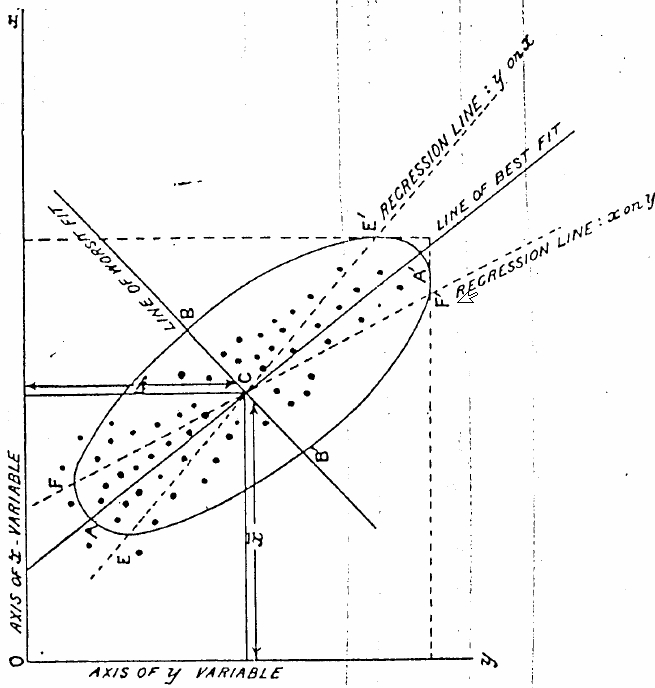
\includegraphics[width=9cm, height=8cm]{pearson}\\
    Wikimedia Commons: Karl Pearson, line of best fit diagram from Philosophical Magazine, 1901.
\end{center}
L'analyse en composantes principales a ses utilités hors du contexte du machine learning, en traitement du signal par exemple où \textit{la méthode des moindres carrés} permet de décomposer toute fonction périodique en une somme de $\cos$ et de $\sin$ plus faciles à traiter. Ceci permettra par exemple \textit{d'échantilloner} un signal continu tel qu'un son pour lui appliquer des traitements avant de le reconstituer. Dès votre premier semestre, en cours d'algèbre linéaire, il est possible que vous traitiez de la \textit{régression linéaire} comme application directe de la méthode des moindres carrés qui y sera présentée. De façon plus générale, l'algèbre linéaire est omniprésente dans le monde scientifique car les matrices permettent de représenter des données quelconques et de les manipuler très facilement.

\noindent Ici, bien entendu, nous n'avons même pas égratigné l'iceberg des applications de l'algèbre linéaire, nous pourrions y passer des heures.

\section{Qu'est-ce que l'algèbre linéaire ?}
C'est, pragmatiquement, une branche des mathématiques très bien comprise, dans le sens : mieux comprise que nombre d'autres qui réservent davantage de mystères et hypothèses pas encore prouvées. On y étudie comment généraliser l'intuition géométrique acquise dans la géométrie planaire et la géométrie dans l'espace, et ce que cette généralisation apporte.\\

\noindent Ce cours introductif, comme le cours d'Algèbre Linéaire de l'EPFL, fera les hypothèses les plus minimes possibles sur vos apprentissages précédents de la matière. Ainsi, nous ne supposerons \textit{pas} que vous savez ce qu'est une matrice, encore moins un espace vectoriel, et nous repartons de zéro dès la section suivante.\\
\chapter{Pré-requis sur les ensembles, fonctions et matrices}

Les trois premiers points de cette sous-section ne concernent pas spécifiquement l'algèbre linéaire mais vous serviront dans tout cours de maths. Vous savez peut-être déjà une grande partie de ce qui suit mais sûrement pas absolument tout.

\section{Opérations élémentaires sur les ensembles, dont le produit cartésien}
Dans ce cours comme tous les cours EPFL hormis ceux traitant justement de théorie des ensembles, nous dirons simplement et naïvement qu'\textbf{un ensemble est une collection d'éléments uniques et non ordonnés}. Dans la suite, nous notons, $A$ étant un ensemble, que $a \in A \iff$ (si et seulement si) l'élément $a$ appartient à l'ensemble $A$.\\

\noindent Pour caractériser un ensemble, il suffit par exemple:
\begin{itemize}
    \item de lister tous ses éléments : $\{1, 2\}$, $\{\text{chaussette rouge, chaussette verte}\}$, ...
    \item de le définir comme \textit{sous-ensemble} d'un ensemble connu en ajoutant une propriété, parfois appelée propriété bâtisseuse notée après une barre verticale : \\ 
    $\{ n \in \mathbb{N} \ | \ n \text{ divise 5}\}$ est l'ensemble des diviseurs naturels de 5, où $\mathbb{N} = \{0, 1, 2, ...\}$. Nous dirons au passage qu'un ensemble $E$ est sous-ensemble d'un ensemble $F$ si $E \subseteq F$, i.e si $E$ est inclus dans $F$, plus explicitement :
    $$E \subseteq F \iff \forall \text{ (pour tout) } e \in E, \ e \in F$$
    
    \item de le construire par union, intersection, complément, différence, produit cartésien entre ensembles.
\end{itemize}
Détaillons le dernier point: 

\begin{boxdef}
Soient deux ensembles $A$ et $B$, sous-ensembles de $X$. Alors nous pouvons définir :
\begin{itemize}
    \item \textit{L'union} de $A$ et $B$, notée $A \cup B = \{x \in X \ | \ x \in A \text{ ou }x \in B\}$.
    \item \textit{L'intersection} de $A$ et $B$, notée $A \cap B = \{x \in X \ | \ x \in A \text{ et } x \in B\}$.
    \item \textit{Le complément} de $A$, notée $\Bar{A} = \{x \in X \ | \ x \notin A\}$.
    \item \textit{La différence} de $A$ et $B$, notée $A \setminus B = A \cap \Bar{B} = \{ x \in X \ | \ x \in A \text{ et } x \not\in B \}$.
    \item \textit{Le produit cartésien} de $A$ et $B$, noté $A \times B = \{(a,b) \ | \ a \in A, b \in B\}$ où $(a,b)$ est une \text{paire ordonnée} - en particulier $(a,b) \neq (b,a)$.
    Pour des ensembles $A_1, A_2,..., A_n$, nous pouvons définir leur produit cartésien ainsi, avec $\Iintv{1, n} = \{i \in \mathbb{N} \ | \ 1 \leq i \text{ et } i \leq n\}$ pour $n \in \mathbb{N}$ : $$A_1 \times A_2 \times ... \times A_n = \{(a_1, a_2, ..., a_n) \ | \ \forall i \in \Iintv{1, n}\ a_i \in A_i\}$$
\end{itemize}
\end{boxdef}

\textbf{\textit{Remarques:}}
\begin{itemize}
    \item On a que $A \cup \Bar{A} = X$ et $A \cap \Bar{A} = \emptyset$, l'ensemble vide.
    \item Le produit cartésien nous intéressera particulièrement dans la suite. Cependant, il faut faire attention: \textit{$A$ n'est \textbf{pas} un sous-ensemble de $A \times B$}, $A \times B$ est constitué de paires, et pas $A$.\\
\end{itemize}


\section{Définition d'une application ensembliste, ou fonction}
Dans cette section, notre seul objectif sera de définir formellement ce qu'est une \textit{application ensembliste}, autrement dit \textit{une fonction}. \\
La notion préliminaire est celle de \textit{relation} entre deux ensembles $A$ et $B$: 
\begin{boxdef}
Nous nommerons tout sous-ensemble $F$ de $A \times B$ une \textit{relation} entre $A$ et $B$. 
\end{boxdef}

Ensuite, nous dirons, concernant cette relation $F$, que :
\begin{boxdef}
$F$ est une \textit{fonction} de $A$ vers $B \iff \forall a \in A\ \exists!$ (il existe un unique) $b := F(a) \in B$ tel que $(a, F(a)) \in F$
Nous notons alors :
\begin{align*}
    F: \ &A \to B\\
    &a \mapsto F(a)
\end{align*}
\end{boxdef}
En d'autres termes, pour chaque $a \in A$, un unique $F(a) \in B$ lui est associé, ce qui devrait correspondre à la définition de fonction donnée au gymnase, au lycée, ...

\section{Injectivité, surjectivité, bijectivité}
\noindent Cette section devrait contenir du contenu nouveau pour beaucoup. \\

\begin{boxdef}
Soit $f: A \to B$ une fonction. Nous définissons son \textit{injectivité} : \\
\begin{center}
    $f$ est \textit{injective} $\iff \forall a_1$ $\in A \, \forall a_2 \in A$, $a_1 \neq a_2 \implies f(a_1) \neq f(a_2)$.
\end{center}
\, \\
De manière équivalente, en usant de la contraposée :\\
\begin{center}
    $f$ est \textit{injective} $\iff \forall a_1 \in A \, \forall a_2 \in A$, $f(a_1) = f(a_2) \implies a_1 = a_2$.
\end{center}
\end{boxdef}

Ceci signifie que pour chaque $b \in B$, il existe \textit{au plus un} $a \in A$ tel que $f(a) = b$. Ainsi, si $A = \{a_1, a_2, a_3\}$ et $B = \{b_1, b_2, b_3, b_4\}$, voici une relation sur $A$ et $B$ définissant une fonction injective :

\begin{center}
\begin{tikzpicture}
  [scale=.6,auto=right]
      \node[vertex] (a1) at (1,10)  {$a_1$};
      \node[vertex] (a2) at (1,8)  {$a_2$};
      \node[vertex] (a3) at (1,6)  {$a_3$};
      \node[vertex] (b1) at (8,10)  {$b_1$};
      \node[vertex] (b2) at (8,8)  {$b_2$};
      \node[vertex] (b3) at (8,6)  {$b_3$};
      \node[vertex] (b4) at (8,4)   {$b_4$};

     \draw[->] (a1)--(b2);
     \draw[->] (a2)--(b3);
     \draw[->] (a3)--(b4);
\end{tikzpicture}
\end{center}

\noindent En effet, à chaque $b_i$ est associé au plus un $a_i$, le fait que $b_1$ n'ait pas d'antécédent ne nuit pas à l'injectivité. Cependant, la relation suivante sur $A$ et $B$ définit bien une fonction, mais pas une fonction injective :

\begin{center}
\begin{tikzpicture}
  [scale=.6,auto=right]
      \node[vertex] (a1) at (1,10)  {$a_1$};
      \node[vertex] (a2) at (1,8)  {$a_2$};
      \node[vertex] (a3) at (1,6)  {$a_3$};
      \node[vertex] (b1) at (8,10)  {$b_1$};
      \node[vertex] (b2) at (8,8)  {$b_2$};
      \node[vertex] (b3) at (8,6)  {$b_3$};
      \node[vertex] (b4) at (8,4)   {$b_4$};

     \draw[->] (a1)--(b2);
     \draw[->] (a2)--(b2);
     \draw[->] (a3)--(b4);
\end{tikzpicture}
\end{center}
Cette relation définit une fonction non injective car il existe 2 $a_i$, $a_1$ et $a_2$, qui ont pour image $b_2$.\\

\noindent Sur des exemples plus réalistes témoignant l'importance des ensembles de départ et d'arrivée :\\
$f: \R \to \R, x \mapsto x^2$ n'est pas injective, car tout réel positif non nul admet 2 antécédents par $f$: $x = f(\sqrt{x}) = f(-\sqrt{x})$. Au passage, $\R$ est l'ensemble des nombres réels.
\begin{center}
\begin{tikzpicture}
    \begin{axis}[
        xmin=-2,xmax=2,
        ymin=-2,ymax=2,
        axis x line=middle,
        axis y line=middle,
        axis line style=->,
        xlabel={$x$},
        ylabel={$y$},
        ]
\addplot[no marks,black,-] expression[domain=-2:2,samples=100]{x^2};
    \end{axis}
\end{tikzpicture}
\end{center}

\noindent Cependant, $g: \R^+ \to \R, x \mapsto x^2$ est bien injective, car nous avons limité le domaine de départ (aussi appelé domaine de définition) afin de faire en sorte qu'au plus un antécédent existe pour toute image.

\begin{center}
\begin{tikzpicture}
    \begin{axis}[
        xmin=0,xmax=2,
        ymin=-2,ymax=2,
        axis x line=middle,
        axis y line=middle,
        axis line style=->,
        xlabel={$x$},
        ylabel={$y$},
        ]
\addplot[no marks,black,-] expression[domain=0:2,samples=100]{x^2};
    \end{axis}
\end{tikzpicture}
\end{center}

\noindent Passons à la seconde définition importante concernant les fonctions, celle de \textit{surjectivité}.\\

\begin{boxdef}
Soit $f: A \to B$ une fonction. Alors: \\
$$f \text{ est \textit{surjective} } \iff \forall b \in B \ \exists \text{ (existe au moins un) }a \in A \text{ tel que } f(a) = b
$$
\end{boxdef}
Ceci signifie... rien de plus que la définition : pour chaque $b \in B$, il existe \textit{au moins} un $a \in A$ tel que $f(a) = b$. Le "au moins" est important, ainsi la fonction suivante est surjective avec $A = \{a_1, ..., a_4\}$ et $B = \{b_1, b_2, b_3\}$ :

\begin{center}
\begin{tikzpicture}
  [scale=.6,auto=right]
      \node[vertex] (a1) at (1,10)  {$a_1$};
      \node[vertex] (a2) at (1,8)  {$a_2$};
      \node[vertex] (a3) at (1,6)  {$a_3$};
      \node[vertex] (a4) at (1,4)  {$a_4$};
      \node[vertex] (b1) at (8,10)  {$b_1$};
      \node[vertex] (b2) at (8,8)  {$b_2$};
      \node[vertex] (b3) at (8,6)  {$b_3$};

     \draw[->] (a1)--(b1);
     \draw[->] (a2)--(b2);
     \draw[->] (a3)--(b3);
     \draw[->] (a4)--(b3);
\end{tikzpicture}
\end{center}
Elle est surjective car au moins un $a_i$ pointe vers chaque $b_j$. Notons qu'elle n'est pas injective car $a_3$ et $a_4$ ont l'image commune $b_3$. Si nous rajoutions un $b_4$ sans lui lier de $a_i$, la fonction obtenue ne serait plus surjective, ce $b_4$ n'admettant pas d'antécédent.\\

\noindent Avant d'arriver à des exemples plus réalistes, définissons \textit{l'ensemble image} d'une fonction $f: A \to B$:
\begin{boxdef}
Soit $f: A \to B$. Étant donné un sous-ensemble $S \subseteq A$, nous définissons : 
$$f(S) = \{b \in B \ | \ \exists s  \in S  \ f(s) = b\}
$$
L'\textit{image} de $f$ sera alors :
$$\Ima(f) = f(A) = \{ b \in B \ | \ \exists a \in A \ f(a) = b \}
$$
\end{boxdef}
Ainsi, étant donnée une telle fonction $f$, nous pouvons restreindre son domaine d'arrivée afin de la rendre surjective : $g: A \to \Ima(f), x \mapsto f(x)$ est surjective par définition.\\

\noindent En fait, nous pouvons même définir la surjectivité autrement mais de manière équivalente grâce à cet ensemble image :

\begin{boxdef}[Une autre définition de la surjectivité]
$$f: A \to B \text{ est surjective } \iff \Ima(f) = B
$$
\end{boxdef}

\noindent Pour retourner à l'exemple de fonctions associant des carrés à des antécédents : soit $f : \R \to \R^+, x \mapsto x^2$, cette fonction est surjective puisque pour tout $x \geq 0 \ \exists y \in \R$ tel que $f(y) = x$, et ce $y = \sqrt{x}$ :
\begin{center}
\begin{tikzpicture}
    \begin{axis}[
        xmin=-2,xmax=2,
        ymin=0,ymax=2,
        axis x line=middle,
        axis y line=middle,
        axis line style=->,
        xlabel={$x$},
        ylabel={$y$},
        ]
\addplot[no marks,black,-] expression[domain=-2:2,samples=100]{x^2};
    \end{axis}
\end{tikzpicture}
\end{center}
La même fonction à laquelle on associerait le domaine d'arrivée $\R$ voire même $\C$ sans changer le domaine de définition deviendrait non surjective, car pour $b = -1$ par exemple, il n'existe pas de $a$ réel tel que $a^2 = -1$.\\

\noindent Dernière définition de cette section, la \textit{bijectivité}:
\begin{boxdef}
Soit $f: A \to B$ une fonction. Alors:
\begin{align*}
    f \text{ est \textit{bijective} } &\iff f \text{ est injective et surjective}\\
    &\iff \forall b \in B\ \exists! a \in A \ f(a) = b
\end{align*}
\end{boxdef}
Pour reprendre une dernière fois nos petites fonctions avec des flèches, avec cette fois $A = \{a_1, a_2, a_3\}$ et $B = \{b_1, b_2, b_3\}$, la fonction suivante est bijective :

\begin{center}
\begin{tikzpicture}
  [scale=.6,auto=right]
      \node[vertex] (a1) at (1,10)  {$a_1$};
      \node[vertex] (a2) at (1,8)  {$a_2$};
      \node[vertex] (a3) at (1,6)  {$a_3$};
      \node[vertex] (b1) at (8,10)  {$b_1$};
      \node[vertex] (b2) at (8,8)  {$b_2$};
      \node[vertex] (b3) at (8,6)  {$b_3$};

     \draw[->] (a1)--(b2);
     \draw[->] (a2)--(b1);
     \draw[->] (a3)--(b3);
\end{tikzpicture}
\end{center}
Elle vérifie bien injectivité et surjectivité. \\
Aussi, pour clore sur les fonctions associant des carrés, la fonction suivante est bijective, où nous avons réduit le domaine de départ pour la rendre injective, puis restreint le domaine d'arrivée pour la rendre surjective :\\
\begin{align*}
    f: \ &\R^+ \to \R^+ \\
    &x \mapsto x^2
\end{align*}
\begin{center}
\begin{tikzpicture}
    \begin{axis}[
        xmin=0,xmax=2,
        ymin=0,ymax=2,
        axis x line=middle,
        axis y line=middle,
        axis line style=->,
        xlabel={$x$},
        ylabel={$y$},
        ]
\addplot[no marks,black,-] expression[domain=0:2,samples=100]{x^2};
    \end{axis}
\end{tikzpicture}
\end{center}

\section{Définitions de $\R^n$, de matrice et du produit matrice-vecteur}
\label{definitionProduitMatVec}
\noindent En algèbre linéaire, la fonction qui nous occupera longtemps - en fait tout le reste de ce cours préparatif - est la suivante, où $n,p \in \mathbb{N}_{\geq 1}$ :
\begin{align*}
    f: \ &\R^n \to \R^p\\
    &x \mapsto f(x) = Ax \text{ où $A$ est une matrice } p \times n
\end{align*}
Décortiquons cette fonction pas à pas.\\
D'abord, nous savons en fait ce qu'est $\R^n$ à présent : 
\begin{boxdef}[Espace $\R^n$]
$$\R^n = \underbrace{\R \times \R \times ... \times \R}_{n \text{ fois}} = \{x=(x_1, x_2, ..., x_n) \ | \ \forall i \in \Iintv{1, n}\ x_i \in \R\}$$
\end{boxdef}
Ainsi, $\R^2 = \R \times \R$ est, géométriquement, l'ensemble des points $(x,y)$ du plan, au même titre que $\R^3$ est l'ensemble des points $(x,y,z)$ de l'espace.\\
Nous nommerons l'ensemble des éléments de $\R^n$ des \textit{vecteurs}. Ainsi, $f$ associe des vecteurs de dimension $n$ à des vecteurs de dimension $p$, ok. Désormais la question est : comment... ?\\
Notons les vecteurs en colonnes ainsi: $x = (a,b,c) = \begin{bmatrix}a \\ b \\ c \end{bmatrix}$. Puis, soit $f: \R^3 \to \R^2$.\\
Considérons $f(x) = f\left(\begin{bmatrix}a \\ b \\ c \end{bmatrix} \right) = \begin{bmatrix}a+5b \\ 3a-b+2c \end{bmatrix}$. Mettons en évidence les coefficients devant $a, b$ et $c$ :
$$\begin{bmatrix}a+5b \\ 3a-b+2c \end{bmatrix} = \begin{bmatrix}1 \cdot a+5\cdot b + 0 \cdot c \\ 3 \cdot a + (-1) \cdot b+2 \cdot c \end{bmatrix} = \underbrace{\begin{bmatrix} 1 & 5 & 0 \\3 & -1 & 2 \end{bmatrix}}_{A_{2 \times 3}} \begin{bmatrix}a \\ b \\ c \end{bmatrix}
$$
Que signifie cette dernière égalité ? Ici, $A$ est une matrice $2 \times 3$, une matrice n'étant rien de plus qu'un tableau (fini) de nombres, ici, réels, de $p$ lignes (ici 2) et $n$ colonnes (ici 3). La dernière égalité use du \textit{produit matrice-vecteur} : En multipliant une matrice de taille $p \times n$ par un vecteur de dimension $n$, nous obtenons un vecteur de dimension $p$ tel que chaque $i$ème \textit{coordonnée} est le \textit{produit scalaire} de la $i$ème ligne de la matrice avec le vecteur. Ainsi :
\begin{boxdef}[Produit matrice-vecteur]
\label{trueDefProduitMatVec}
\, \begin{align*}
Ax = \begin{bmatrix} a_{1,1} & a_{1,2} & \cdots & a_{1, n} \\ a_{2,1} & a_{2,2} & \cdots & a_{2, n} \\ \vdots & \ddots & & \vdots \\ a_{p,1} & \cdots & \cdots & a_{p,n} \end{bmatrix}\begin{bmatrix} x_1 \\ x_2 \\ \vdots \\ x_n \end{bmatrix}
&= \begin{bmatrix} a_{1,1}x_1 + a_{1,2}x_2 + a_{1,3}x_3 + ... + a_{1, n}x_n \\ a_{2,1}x_1 + a_{2,2}x_2 + a_{2,3}x_3 + ... + a_{2, n}x_n \\ \vdots \\ a_{p,1}x_1 + a_{p,2}x_2 + a_{p,3}x_3 + ... + a_{p, n}x_n \end{bmatrix} \\
&=  \left[\sum_{k = 1}^n a_{i,k}x_k\right]_{i \in \Iintv{1,p}}
\end{align*}
\end{boxdef}
Notons tout de suite que dans la fonction proposée $f: \R^n \to \R^p, x \mapsto Ax$, $n$ est le nombre de \textit{colonnes} de $A$ et $p$ son nombre de \textit{lignes}. En effet, une matrice prend des vecteurs de dimension son nombre de colonnes pour les associer à des vecteurs de dimension son nombre de lignes, donc l'application $f$ associée que nous nommerons \textit{application matricielle} ou fonction matricielle dans la suite a pour domaine de définition les vecteurs de dimension le nombre de colonnes, et pour domaine d'arrivée les vecteurs de dimension le nombre de lignes.\\

\noindent Remarquons qu'une matrice \textit{n'est pas} une simple notation, mais est bien un objet mathématique en tant que tel, qui pourrait être précisé ainsi : si $b_1, ..., b_n$ sont les colonnes d'une matrice $B$ de taille $p \times n$ - donc des vecteurs de dimension $p$, nous pourrions poser que $B = (b_1, ..., b_n)$ ainsi $B \in (\R^p)^n$ vu que $B$ est un $n$-tuple d'éléments d'un certain ensemble $E$, et $E$ se trouve être $\R^p$. Ceci donne une définition plus rigoureuse que celle d'un tableau de $pn$ entrées, mais nous privilégions néanmoins la notation du tableau car elle est plus intuitive. \\
Pour cette raison, nous notons l'ensemble des matrices de taille $p \times n$ à coefficients réels ainsi : $\R^{p \times n}$.\\
\chapter{Systèmes linéaires}

\noindent Voyons ici une première application importante des objets mathématiques introduits dans la section précédente, les matrices : les \textit{systèmes d'équations linéaires}. Tout d'abord qu'est ce qu'une équation linéaire ? Il s'agit d'une égalité faisant intervenir une somme d'inconnues chacune multipliées par un coefficient réel. 

\section{Définition et exemples, intuition géométrique}
\begin{boxdef}
\noindent Une \textit{équation linéaire} est une équation de la forme : 
$$a_1 x_1 + ... + a_n x_n = b$$
avec $\{a_i \}_{i \in \Iintv{1,n}} \subseteq \mathbb{R}$ et $b\in \mathbb{R}$. Nous appelons $n$ le nombre \textit{d'inconnues}. Un \textit{système} d'équations linéaires est caractérisé par un ensemble \textit{fini} d'équations linéaires.
\end{boxdef}
Plus précisément nous pouvons donc représenter une équation linéaire sous la forme :
$$a_1 x_1 + ... + a_n x_n = b
$$
où les $a_i \in \R$ et $b \in \R$ sont connus, puis écrire un système linéaire :
$$\begin{cases} a_{1,1}x_1 + a_{1,2}x_2 + a_{1,3}x_3 + ... + a_{1, n}x_n = b_1 \\ a_{2,1}x_1 + a_{2,2}x_2 + a_{2,3}x_3 + ... + a_{2, n}x_n =b_2 \\ \vdots \\ a_{p,1}x_1 + a_{p,2}x_2 + a_{p,3}x_3 + ... + a_{p, n}x_n = b_p \end{cases}$$

\, \\
Avant de continuer, un peu de vocabulaire:
\begin{boxdef}
Un système linéaire à $n$ inconnues et $p$ équations est dit \textit{homogène} si $b_i = 0$ $\forall i \in \Iintv{1, p}$.
\end{boxdef}

\noindent Le plus souvent, la donnée intéressante d'un système d'équations linéaires est son ensemble de solutions, c'est à dire le tuple des $(y_1, y_2, \ldots, y_n)\in \mathbb{R}^n$ tels que pour chaque équation du système, en injectant ces valeurs dans les $x_n$ on obtienne bien $b_i$. Notons pour l'instant cet ensemble de solutions $S(\{a_{i,j}\},b)$. Concentrons-nous sur quelques équations simples pour visualiser géométriquement à quoi ressemblent ces ensembles de solutions.\\

\noindent Tout d'abord remarquons que pour un système d'équations à $n$ variables, $S(\{a_{i,j}\}, b)$ est un sous ensemble de $\mathbb{R}^n$ puisqu'il est constitué de $n$-uplets de réels. Commençons donc avec des sous ensembles de $\mathbb{R}^2$, à savoir des sous ensembles du plan. 
$$ 2x_1 - x_2 = 0 $$
\noindent Ceci est l'équation d'une droite. Ici nous commençons par remarquer qu'il s'agit d'un système à une équation et deux variables, nous avons, selon la notation précédente $a_{1,1} =2 $, $a_{1,2} = -1$ et  $b_1 = 0$. Remarquons qu'il s'agit d'un système homogène. Nous résolvons en passant simplement le $x_2$ de l'autre coté on obtient :
$$2x_1 = x_2$$
Il s'agit donc de l'ensemble des $(x_1, x_2) \in \mathbb{R}^2$ tels que $2x_1 = x_2$. Nous pourrons alors aussi dire qu'il s'agit, pour tout $x\in \mathbb{R}$ des $(x, 2x)$. Géométriquement à quoi correspond cet ensemble ? Remarquons que comme $x$ est réel il s'agit bien de l'ensemble des $\left\{x\begin{bmatrix}1 \\ 2 \end{bmatrix} \ | \ x \in \R\right\}$. Visuellement le vecteur $\begin{bmatrix}1 \\ 2 \end{bmatrix}$ est représenté ci dessous. L'ensemble des vecteurs obtenus en lui multipliant un réel $x$ sont représentés sur la figure de droite:
\begin{center}
\begin{tikzpicture}

  \draw[thin,gray!40] (-3,-3) grid (3,3);
  \draw[<->] (-3,0)--(3,0) node[right]{$x$};
  \draw[<->] (0,-3)--(0,3) node[above]{$y$};
  \draw[line width=2pt,blue,-stealth](0,0)--(1,2) node[anchor=south west]{$\begin{bmatrix}1 \\ 2 \end{bmatrix}$};
\end{tikzpicture}
\hspace{2CM}
\begin{tikzpicture}
  \draw[thin,gray!40] (-3,-3) grid (3,3);
  \draw[<->] (-3,0)--(3,0) node[right]{$x$};
  \draw[<->] (0,-3)--(0,3) node[above]{$y$};
    \draw[line width=2pt,red,-stealth](0,0)--(1.5,3) node[anchor=south west]{};
  \draw[line width=2pt,blue,-stealth](0,0)--(1,2) node[anchor=south west]{};
  \draw[line width=2pt,red,-stealth](0,0)--(-1.5,-3) node[anchor=south west]{};

\end{tikzpicture}
\end{center}
Il s'agit donc d'une droite dirigée par le vecteur $\begin{bmatrix}1 \\ 2 \end{bmatrix}$. Prenons désormais un exemple avec un système à trois inconnues et deux équations :

$$ \begin{cases}3x_1 + 2x_2 + x_3 = 2\\x_1 + 2x_2 + x_3 = 2 \end{cases}$$
%yeet
%who is the author of this yeet?
Comment procéder à la résolution ? Soustrayons la deuxième équation à la première pour obtenir :

$$ \begin{cases}2x_1  = 0\\ x_1 + 2x_2 + x_3 = 2 \end{cases}$$

\noindent Et donc conclure déjà que les points de notre ensemble de solution seront de la forme $(0, x_2, x_3)\in \mathbb{R}^3$ en divisant des deux cotés de $ 2x_1  = 0$ par $2$. Remplaçons donc $x_1$ par $0$ dans la seconde équation pour obtenir :
$$ 2x_2 + x_3 = 2 $$
\noindent Il s'agit encore une fois de l'équation d'une droite, ici de la droite dirigée par $$\begin{bmatrix}0 \\ 1 \\ -2 \end{bmatrix}$$ mais décalée de $2$ au niveau de l'origine :
\\
\begin{tikzpicture}

\pgfplotsset{
colormap={whitered}{color(0cm)=(white); color(1cm)=(orange!75!red)}
}

\begin{axis}[  colormap name=whitered,   view={45}{65},     width=10cm]
\addplot3[variable=t, mesh, draw=red!50, domain=-2:2] (0,{t + 2},{-2*t});
\end{axis}
\end{tikzpicture}
\hspace{1CM}
\begin{tikzpicture}
  \draw[thin,gray!40] (-3,-3) grid (3,3);
  \draw[<->] (-3,0)--(3,0) node[right]{$x$};
  \draw[<->] (0,-3)--(0,3) node[above]{$y$};
    \draw[line width=2pt,red,-stealth](-0.5,3)--(2.5,-3) node[anchor=south west]{};

\end{tikzpicture}
A droite est une coupe selon l'axe des $x_1 = 0$. 
\section{L'équation $Ax = b$}
\noindent Reprenons une équation connue et cherchons les informations capitales à son sujet : 
$$ \begin{cases}5x_1 + x_3 = \sqrt{2}\\x_1 + 3x_2 +4x_3 = 3\end{cases} $$
\noindent Quelles sont les informations minimales dont on a besoin pour reconstituer une telle équation ? Les variables peuvent être ordonnées de sorte à toujours apparaître dans le même ordre. Nous pourrions aussi omettre le signe "$=$" en sachant que le dernier coefficient est celui correspondant à $b_i$. Enfin nous pourrions encore omettre le nom des variables et ne conserver que les coefficients puisque l'ordre des coefficients détermine la variable qu'ils multiplient. Et que faire si l'une des variables n'est pas présente ? Il s'agit bien de la multiplication par $0$ dans ce cas. En résumé nous obtenons :
$$ 5 \quad 0 \quad 1 \quad \sqrt{2}$$
$$ 1 \quad 3 \quad 4 \quad 3 $$
Nous pouvons réécrire cela de manière plus élégante sous la forme :
$$ 
\left[
\begin{array}{@{}ccc|c@{}}
5 & 0 & 1 & \sqrt{2} \\
1 & 3 & 4 & 3 \\
\end{array}
\right]
$$
\noindent Voici la forme \textit{matricielle augmentée} d'un système linéaire. Cette forme est équivalente à la donnée de l'équation suivante dite \textit{équation matricielle} $Ax = b$ :
$$\underbrace{\begin{bmatrix}
5 & 0 & 1 \\
1 & 3 & 4 
\end{bmatrix}}_{A}\underbrace{\begin{bmatrix}
x_1 \\ x_2 \\ x_3
\end{bmatrix}}_{x} = \underbrace{\begin{bmatrix}
\sqrt{2} \\ 2
\end{bmatrix}}_{b}
$$
Dans cette notation, $A$ est la \textit{matrice des coefficients}, et la \textit{matrice augmentée} de l'équation matricielle est ainsi $\begin{bmatrix}
A & | & b
\end{bmatrix}$.

Cela aboutit à cette définition générale:
\begin{boxdef}
Étant donné un système linéaire
$$\begin{cases} a_{1,1}x_1 + a_{1,2}x_2 + a_{1,3}x_3 + ... + a_{1, n}x_n = b_1 \\ a_{2,1}x_1 + a_{2,2}x_2 + a_{2,3}x_3 + ... + a_{2, n}x_n =b_2 \\ \vdots \\ a_{p,1}x_1 + a_{p,2}x_2 + a_{p,3}x_3 + ... + a_{p, n}x_n = b_p \end{cases}$$
On note $b \in \R^p$ le vecteur formé par les $b_i$ et on défini la \textit{matrice des coefficients} comme étant
$$A = \begin{bmatrix}
a_{1,1} & a_{1,2} & \cdots & a_{1,n} \\
a_{2,1} & a_{2,2} & \cdots & a_{2,n} \\
\vdots & \vdots & \ddots & \vdots \\
a_{p,1} & a_{p,2} & \cdots & a_{p,n} \\
\end{bmatrix}$$
La \textit{matrice augmentée} du système est donc $\begin{bmatrix}
A & | & b
\end{bmatrix}$.
\end{boxdef}

\section{Réduction et échelonnage}
\noindent Soit le système linéaire :
$$\begin{cases}
3x_1 + 2x_2 + x_3 = 2\\
x_1 + 2x_2 + x_3 = 2
\end{cases}
$$
La matrice augmentée associée est alors :
$$ 
\left[
\begin{array}{@{}ccc|c@{}}
3 & 2 & 1 & 2 \\
1 & 2 & 1 & 2 \\
\end{array}
\right]
$$
Résolvons ce système sous les deux écritures i.e système et matrice augmentée simultanément. Soustrayons donc chaque coefficient de la seconde ligne au coefficient correspondant de la ligne supérieure pour obtenir :
$$ 
\left[
\begin{array}{@{}ccc|c@{}}
3 \color{red} - 1 & 2 \color{red} -2 & 1  \color{red} - 1 & 2 \color{red} - 2 \\
1 & 2 & 1 & 2 \\
\end{array}
\right] 
\iff 
\begin{cases}
(3\textcolor{red}{-1})x_1 + (2\textcolor{red}{-2})x_2 + (1\textcolor{red}{-1})x_3 = 2\textcolor{red}{-2}\\
x_1 + 2x_2 + x_3 = 2
\end{cases}
$$

$$ 
\left[
\begin{array}{@{}ccc|c@{}}
2 & 0 & 0 & 0 \\
1 & 2 & 1 & 2 \\
\end{array}
\right]
\iff
\begin{cases}
2x_1 = 0\\
x_1 + 2x_2 + x_3 = 2
\end{cases}
$$
Nous multiplions ensuite les coefficients de la première ligne par $\color{blue}\frac{1}{2}$ :
$$ 
\left[
\begin{array}{@{}ccc|c@{}}
2 \color{blue}\times\frac{1}{2}  & 0 & 0 & 0 \\
1 & 2 & 1 & 2 \\
\end{array}
\right]
\iff
\begin{cases}
2\textcolor{blue}{\times \frac{1}{2}}x_1 = 0\\
x_1 + 2x_2 + x_3 = 2
\end{cases}
$$
$$ 
\left[
\begin{array}{@{}ccc|c@{}}
1 & 0 & 0 & 0 \\
1 & 2 & 1 & 2 \\
\end{array}
\right]
\iff
\begin{cases}
x_1 = 0 \\
x_1 + 2x_2 + x_3 = 2
\end{cases}
$$
Et nous concluons alors que le premier coefficient est nul.\\
Continuons en soustrayant la première ligne à la seconde :
$$ 
\left[
\begin{array}{@{}ccc|c@{}}
1 & 0 & 0 & 0 \\
1\color{red} - 1 & 2\color{red} - 0 & 1\color{red} - 0 & 2\color{red} - 0 \\
\end{array}
\right]
\iff 
\begin{cases}
x_1 = 0 \\
(1\textcolor{red}{-1})x_1 + (2\textcolor{red}{-0})x_2 + (1\textcolor{red}{-0})x_3 = 2\textcolor{red}{-0}
\end{cases}
$$
$$ 
\left[
\begin{array}{@{}ccc|c@{}}
1 & 0 & 0 & 0 \\
0 & 2 & 1 & 2 \\
\end{array}
\right]
\iff
\begin{cases}
x_1 = 0 \\
2x_2 + x_3 = 2
\end{cases}
$$
Nous pouvons peut être aller un peu plus loin en divisant la deuxième ligne par 2, ce qui donne :
$$
\left[
\begin{array}{@{}ccc|c@{}}
1 & 0 & 0 & 0 \\
0 & 1 & \frac{1}{2} & 1 \\
\end{array}
\right]
\iff
\begin{cases}
x_1 = 0 \\
x_2 + \frac{1}{2}x_3 = 1
\end{cases}
$$
Formalisons les opérations que nous pouvons utiliser pour résoudre un système linéaire sous sa forme matricielle, qui sont en fait les mêmes que celle sous sa forme de système d'équations linéaires : 
\begin{itemize}
    \item \textit{La multiplication par un réel non nul} d'une ligne complète (ne pas oublier le $b_i$).
    \item \textit{Additionner deux lignes} (la soustraction correspond à multiplier la ligne par $-1$ puis l'additionner à l'autre et la multiplier à nouveau par $-1$).
    \item \textit{Permuter deux lignes}, la permutation de deux équations dans un système étant sans conséquence.
\end{itemize}
\textbf{Notons d'abord que ces trois opérations sont réversibles. C'est ce qui fait que l'ensemble des solutions n'est pas changé par ces 3 opérations.}\\

\noindent Remarquons aussi que nous pouvons toujours procéder comme dans la soustraction et multiplier la $i$ème ligne par un réel $\lambda \in \mathbb{R}^*$, l'additionner à la $j$-ème ligne et multiplier à nouveau la $i$ème ligne par $\frac{1}{\lambda}$. Nous en concluons une règle composite très pratique : 
\begin{itemize}
    \item \textit{La multiplication puis l'addition} d'une ligne vers une autre sans modifier sa propre valeur.
\end{itemize}
Il s'agit désormais de trouver un algorithme qui pourrait toujours mener vers la forme la plus réduite possible d'une équation, commençons par trouver les critères qu'une telle forme doit posséder. Tout d'abord on remarque que les lignes de la forme 
$$ 
\left[
\begin{array}{@{}ccccc|c@{}}
0 & \ldots & \lambda & \ldots & 0 & \sigma \\
\end{array}
\right]
\iff
0x_1 + \cdots + \lambda x_i + 0x_{i+1} + \cdots + 0x_n = \sigma
$$
pour tout $\lambda \in \R^*, \sigma \in \mathbb{R}$ sont très pratiques puisqu'elles déterminent la valeur de la variable dont le coefficient n'est pas nul de manière unique : $x_i = \frac{\sigma}{\lambda}$. Il s'agirait donc d'obtenir une matrice qui maximise le nombre de ligne de cette forme.\\

\noindent Remarquons que si nous disposons d'une ligne de la forme :
$$ 
\left[
\begin{array}{@{}ccccc|c@{}}
0 & \ldots & \lambda_1 & \ldots & \lambda_n & \sigma \\
\end{array}
\right]
$$
\noindent Alors pour annuler les derniers coefficients (sur la droite) il faut déjà avoir une ligne qui contienne au plus autant de coefficients non nuls à droite sans quoi lors de l'addition des lignes nous créerons des termes non nuls là où nous avions déjà des termes nuls :
$$ 
\left[
\begin{array}{@{}ccccc|c@{}}
0 \color{green} -0  & 0\color{green} -0 & \lambda_1 \color{green} -\alpha_1 & \lambda_2 \color{green} -\alpha_2 & \lambda_3\color{green} -\alpha_3 & \sigma_1\color{green} -\sigma_2 \\
0 & 0  & \alpha_1 & \alpha_2 & \alpha_3 & \sigma_2 \\
\end{array}
\right]
$$
Ci-dessus une soustraction n'ajoutant pas de termes, et ci après une soustraction ajoutant des termes non nuls.
$$ 
\left[
\begin{array}{@{}ccccc|c@{}}
0 \color{green} -0  & 0\color{red} -\alpha_0 & \lambda_1 \color{green} -\alpha_1 & \lambda_2 \color{green} -\alpha_2 & \lambda_3\color{green} -\alpha_3 & \sigma_1\color{green} -\sigma_2 \\
0 & \alpha_0  & \alpha_1 & \alpha_2 & \alpha_3 & \sigma_2 \\
\end{array}
\right]
$$
Nous constatons donc que pour arriver à obtenir une forme matricielle contenant le plus de lignes avec un seul terme non nul il conviendrait premièrement d'en trouver une dont les lignes auraient un \textit{nombre de termes non nul à droite décroissant}, c'est-à-dire telle que : si $A \in \R^{p \cross n}$, alors pour tout $i \in \Iintv{1,p}$, si la colonne $k\in \Iintv{1,n}$ est la première colonne de la $i$ème ligne dont le coefficient est non nul, alors le rang de la première colonne de la $i+1$ème ligne dont le coefficient est non nul est strictement supérieur à $k$. \\

Dans la matrice suivante, $*$ désigne un coefficient arbitraire, et les $\Delta_i$ désignent des coefficients \textit{non nuls} arbitraires.
$$\begin{bmatrix}
0 & \cdots & 0 & \Delta_1 & * & \cdots & * & * & *\\
0 &\cdots & 0 & 0 & \cdots & \Delta_2 & * &\cdots & *\\
\vdots &&&&&&&&\vdots \\
0 & &&\cdots&&\cdots&&& *
\end{bmatrix}
$$
\begin{boxdef}
La forme ci-dessus est appelée la forme \textit{échelonnée} d'une matrice. Les premiers termes non nuls sur une ligne sont appelés \textit{pivots}.
\end{boxdef}
En d'autres termes, les coefficients non nuls font une sorte d'escalier plus ou moins régulier. Des exemples de matrices sous forme échelonnée, avec, en bleu, les pivots :
$$
\begin{bmatrix}
\color{blue}5 & 0 & 3 & 3 \\
0 & 0 & \color{blue}2 & 1 \\
0 & 0 & 0 & 0
\end{bmatrix},
\begin{bmatrix}
0 & 0 \\
0 & 0
\end{bmatrix},
\begin{bmatrix}
\color{blue}1 & 0\\
0 & \color{blue}1\\
0 & 0
\end{bmatrix},
\begin{bmatrix}
0 & 0 & 0 & 0 & 0 \\
0 & 0 & 0 & \color{blue}5 & 4
\end{bmatrix}
$$
Des exemples de matrices \textit{pas} sous forme échelonnée :
$$
\begin{bmatrix}
0 & 2 & 3 \\
1 & 5 & 6\\
0 & 9 & 1
\end{bmatrix},
\begin{bmatrix}
0 & 0 & 7 \\
0 & 4 & 0\\
0 & 0 & 0\\
0 & 0 & 0
\end{bmatrix}
$$
La première n'est pas échelonnée car le coefficient $1$ est en colonne $1$ de la ligne 2, soit avant le premier coefficient non nul de la ligne au-dessus, qui est $2$. Idem : le $4$ dans la seconde matrice est situé à la deuxième colonne alors que la première ligne compte le coefficient non nul 7 à la troisième colonne.\\

\noindent Ensuite, étant donnée une forme échelonnée, il est encore possible de la réduire. Nous pouvons faire en sorte que tous les pivots valent $1$ et que tous les coefficients sur la même colonne au-dessus de chaque pivot deviennent nuls, et ce \textit{en divisant la ligne du pivot} par le pivot lui-même (non nul par définition), puis en soustrayant la ligne du pivot aux lignes du dessus. Ainsi, il faudra commencer par la ligne du-dessous.\\
\begin{boxdef}
Nous appelons cette forme celle de matrice \textit{échelonnée réduite}.\\
\end{boxdef}
Des exemples rendront ce texte cryptique  plus compréhensible :
\begin{align*}
\begin{bmatrix}
\color{blue}5 & 0 & 3 & 3\\
0 & 0 & \color{blue}2 & 1\\
0 & 0 & 0 & 0
\end{bmatrix} \overset{L_2 \to  \frac{1}{2}L_2}{\sim} 
&\begin{bmatrix}
\color{blue}5 & 0 & 3 & 3\\
0 & 0 & \color{blue}1 & \frac{1}{2}\\
0 & 0 & 0 & 0
\end{bmatrix}\\
\overset{L_1 \to L_1 - 3L_2}{\sim}
&\begin{bmatrix}
\color{blue}5 & 0 & 0 & \frac{3}{2}\\
0 & 0 & \color{blue}1 & \frac{1}{2}\\
0 & 0 & 0 & 0
\end{bmatrix}\\
\overset{L_1 \to \frac{1}{5}L_1}{\sim}
&\begin{bmatrix}
\color{blue}1 & 0 & 0 & \frac{3}{10}\\
0 & 0 & \color{blue}1 & \frac{1}{2}\\
0 & 0 & 0 & 0
\end{bmatrix}
\end{align*}
Puis, $\begin{bmatrix}
0 &0\\
0 & 0
\end{bmatrix}$ est déja échelonnée réduite. Idem, la matrice $\begin{bmatrix}
1 & 0\\
0 & 1\\
0 & 0
\end{bmatrix}$ l'est déjà aussi. Enfin :
\begin{align*}
\begin{bmatrix}
0 & 0 & 0 & 0 & 0 \\
0 & 0 & 0 & \color{blue}5 & 4
\end{bmatrix}
\overset{L_2 \to \frac{1}{5}L_2}{\sim}
\begin{bmatrix}
0 & 0 & 0 & 0 & 0 \\
0 & 0 & 0 & \color{blue}1 & \frac{4}{5}
\end{bmatrix}
\end{align*}
Nous verrons dans la prochaine section comment exploiter cette forme échelonnée réduite afin d'expliciter l'ensemble des solutions d'un système linéaire.\\

\noindent Il serait désormais utile de trouver un algorithme amenant à une forme échelonnée, puisque nous savons passer d'une forme échelonnée à une forme réduite désormais. La méthode présentée ci-après est celle du \textit{pivot de Gauss}.\\

\noindent Nous commencerons par un exemple. Calculons la forme échelonnée réduite de la matrice suivante :
$$\begin{bmatrix}
-1 & -2 & -1 & 3 \\
-2 & -3 &  0 & 3 \\
1  &  4 &  5 & -9
\end{bmatrix}
$$
\begin{mdframed}
Le but sera d'aller de la gauche vers la droite. Pour chaque colonne, nous sélectionnerons une ligne que nous trouverions "avantageuse" afin de simplifier les calculs, bien qu'en soi n'importe quelle ligne marcherait. Cette ligne sera placée au-dessus. Puis, nous ajoutons des multiples de cette ligne aux lignes en-dessous de manière à faire apparaître des 0 dans la colonne courante. Puis, nous bloquons la ligne du dessus et passons à la prochaine colonne jusqu'à avoir traité la colonne la plus à droite.
\end{mdframed}

\noindent Ici, en choisissant la 3ème ligne dans la matrice ci-dessus, i.e celle contenant un coefficient $1$ à sa gauche, nous pourrions simplement annuler le $-1$ et le $-2$ en ajoutant respectivement 1 et 2 fois la ligne 3. Au fur et à mesure, les pivots bloqués seront colorés en bleu.\\

\noindent Chaque chose en son temps. Mettons d'abord en évidence cette ligne 3 en la plaçant au-dessus :
$$\begin{bmatrix}
-1 & -2 & -1 & 3 \\
-2 & -3 &  0 & 3 \\
1  &  4 &  5 & -9
\end{bmatrix}
\overset{L_1 \leftrightarrow L_3}{\sim} 
\begin{bmatrix}
\color{blue}1  &  4 &  5 & -9\\
-2 & -3 &  0 & 3 \\
-1 & -2 & -1 & 3 
\end{bmatrix}
$$
Ensuite, faisons des $0$ apparaître sous ce premier futur pivot :
\begin{align*}
\begin{bmatrix}
\color{blue}1  &  4 &  5 & -9\\
-2 & -3 &  0 & 3 \\
-1 & -2 & -1 & 3 
\end{bmatrix}
\overset{L_2 \to L_2 + 2L_1}{\sim}
&\begin{bmatrix}
\color{blue}1  &  4 &  5 & -9\\
0 & 5 &  10 & -15 \\
-1 & -2 & -1 & 3 
\end{bmatrix}\\
\overset{L_3 \to L_3 + L_1}{\sim}
&\begin{bmatrix}
\color{blue}1  &  4 &  5 & -9\\
0 & 5 &  10 & -15 \\
0 & 2 & 4 & -6 
\end{bmatrix}
\end{align*}
Nous pourrions recommencer directement l'opération avec la seconde colonne comme le prescrit la méthode de Gauss, mais remarquons d'abord que les lignes 2 et 3 se ressemblent particulièrement et sont toutes deux multiples de $\begin{bmatrix}
0 & 1 & 2 & -3
\end{bmatrix}$, mettons cela en évidence :
\begin{align*}
\begin{bmatrix}
\color{blue}1  &  4 &  5 & -9\\
0 & 5 &  10 & -15 \\
0 & 2 & 4 & -6 
\end{bmatrix}
\overset{L_3 \to \frac{1}{2}L_3}{\sim}
&\begin{bmatrix}
\color{blue}1  &  4 &  5 & -9\\
0 & 5 &  10 & -15 \\
0 & 1 & 2 & -3 
\end{bmatrix}\\
\overset{L_2 \to \frac{1}{5}L_2}{\sim}
&\begin{bmatrix}
\color{blue}1  &  4 &  5 & -9\\
0 & 1 & 2 & -3 \\
0 & 1 & 2 & -3 
\end{bmatrix}
\end{align*}
Il ne reste plus qu'à \textbf{yeet} la 2ème ligne - c'est un terme technique signifiant soustraire la 3ème à la 2ème \, ;)
$$
\begin{bmatrix}
\color{blue}1  &  4 &  5 & -9\\
0 & 1 & 2 & -3 \\
0 & 1 & 2 & -3 
\end{bmatrix}
\overset{L_2 \to L_2 - L_3}{\sim}
\begin{bmatrix}
\color{blue}1  &  4 &  5 & -9\\
0 & 0 & 0 & 0 \\
0 & 1 & 2 & -3 
\end{bmatrix}
$$
Nous avons presque une forme échelonnée ! Il reste encore à permuter les deux dernières lignes :
$$
\begin{bmatrix}
\color{blue}1  &  4 &  5 & -9\\
0 & 0 & 0 & 0 \\
0 & 1 & 2 & -3 
\end{bmatrix}
\overset{L_2 \leftrightarrow L_3}{\sim}
\begin{bmatrix}
\color{blue}1  &  4 &  5 & -9\\
0 & \color{blue}1 & 2 & -3 \\
0 & 0 & 0 & 0
\end{bmatrix}
$$
Enfin, pour arriver à la forme échelonnée réduite, en faisant donc apparaître un 0 au-dessus du second (et dernier) pivot, il suffira de retrancher la ligne 2 à la première ligne 4 fois :
$$
\begin{bmatrix}
\color{blue}1  &  4 &  5 & -9\\
0 & \color{blue}1 & 2 & -3 \\
0 & 0 & 0 & 0
\end{bmatrix}
\overset{L_1 \to L_1 - 4L_2}{\sim}
\begin{bmatrix}
\color{blue}1  &  0 &  -3 & 3\\
0 & \color{blue}1 & 2 & -3 \\
0 & 0 & 0 & 0
\end{bmatrix}
$$

\noindent Encore un exemple, issu du Lay, le livre de cours, que nous recommandons d'ailleurs pour son cours très clair, ses exemples d'applications de méthodes calculatoires proprement expliquées, mais pas pour ses exercices plus théoriques pour lesquels il faudra privilégier les séries d'exercices. Ceci est l'exemple 3 de la section 1.2 : Méthode du pivot de Gauss et formes échelonnées, qui est expliqué différemment dans le livre, et nous vous invitons à comparer sa méthode à celle présentée ci-après. \\

\noindent Trouvons la forme échelonnée réduite de la matrice suivante :
$$
\begin{bmatrix}
 0 &  3 & -6 &  6 &  4 & -5\\
 3 & -7 &  8 & -5 &  8 &  9\\
 3 & -9 & 12 & -9 &  6 & 15
\end{bmatrix}
$$
Avant de commencer, la troisième ligne est simplifiable par 3.
$$
\begin{bmatrix}
 0 &  3 & -6 &  6 &  4 & -5\\
 3 & -7 &  8 & -5 &  8 &  9\\
 3 & -9 & 12 & -9 &  6 & 15
\end{bmatrix}
\overset{L_3 \to \frac{1}{3}L_3}{\sim}
\begin{bmatrix}
 0 &  3 & -6 &  6 &  4 & -5\\
 3 & -7 &  8 & -5 &  8 &  9\\
 1 & -3 &  4 & -3 &  2 & 5
\end{bmatrix}
$$
Il sera plus aisé de multiplier la 3ème ligne par 3 avant de la soustraire à la seconde que de multiplier la 2ème ligne par $\frac{1}{3}$ puis la soustraire à la 3ème. Ainsi, ce $1$ dans la première colonne deviendra notre futur pivot, permutons les lignes en conséquence :
$$
\begin{bmatrix}
 0 &  3 & -6 &  6 &  4 & -5\\
 3 & -7 &  8 & -5 &  8 &  9\\
 1 & -3 &  4 & -3 &  2 & 5
\end{bmatrix}
\overset{L_3 \leftrightarrow L_1}{\sim}
\begin{bmatrix}
 \color{blue}1 & -3 &  4 & -3 &  2 & 5\\
 3 & -7 &  8 & -5 &  8 &  9\\
 0 &  3 & -6 &  6 &  4 & -5
\end{bmatrix}
$$
Ôtons alors ce coefficient $3$ d'en-dessous du futur pivot :
$$
\begin{bmatrix}
 \color{blue}1 & -3 &  4 & -3 &  2 & 5\\
 3 & -7 &  8 & -5 &  8 &  9\\
 0 &  3 & -6 &  6 &  4 & -5
\end{bmatrix}
\overset{L_2 \to L_2 - 3L_1}{\sim}
\begin{bmatrix}
 \color{blue}1 & -3 &  4 & -3 &  2 & 5\\
 0 & 2 &  -4 & 4 &  2 &  -6\\
 0 &  3 & -6 &  6 &  4 & -5
\end{bmatrix}
$$
Ici aussi, nous remarquons que la seconde ligne peut être simplifiée par 2 :
$$
\begin{bmatrix}
 \color{blue}1 & -3 &  4 & -3 &  2 & 5\\
 0 & 2 &  -4 & 4 &  2 &  -6\\
 0 &  3 & -6 &  6 &  4 & -5
\end{bmatrix}
\overset{L_2 \to \frac{1}{2}L_2}{\sim}
\begin{bmatrix}
 \color{blue}1 & -3 &  4 & -3 &  2 & 5\\
 0 & 1 &  -2 & 2 &  1 &  -3\\
 0 &  3 & -6 &  6 &  4 & -5
\end{bmatrix}
$$
Ce $1$ en deuxième colonne sera donc notre prochain pivot. Reste à \textbf{YEET} la troisième ligne :
$$
\begin{bmatrix}
 \color{blue}1 & -3 &  4 & -3 &  2 & 5\\
 0 & 1 &  -2 & 2 &  1 &  -3\\
 0 &  3 & -6 &  6 &  4 & -5
\end{bmatrix}
\overset{L_3 \to L_3 - 3L_2}{\sim}
\begin{bmatrix}
 \color{blue}1 & -3 &  4 & -3 &  2 & 5\\
 0 & \color{blue}1 &  -2 & 2 &  1 &  -3\\
 0 &  0 & 0 &  0 &  \color{blue}1 & 4
\end{bmatrix}
$$
Et nous aboutissons ainsi à une forme échelonnée. Afin de la rendre réduite, nous commençons par le pivot le plus à droite puis nous supprimons les coefficients non-nuls au-dessus de ce pivot.
\begin{align*}
\begin{bmatrix}
 \color{blue}1 & -3 &  4 & -3 &  2 & 5\\
 0 & \color{blue}1 &  -2 & 2 &  1 &  -3\\
 0 &  0 & 0 &  0 &  \color{blue}1 & 4
\end{bmatrix}
\overset{L_2 \to L_2 - L_3}{\sim}
&\begin{bmatrix}
 \color{blue}1 & -3 &  4 & -3 &  2 & 5\\
 0 & \color{blue}1 &  -2 & 2 &  0 &  -7\\
 0 &  0 & 0 &  0 &  \color{blue}1 & 4
\end{bmatrix}\\
\overset{L_1 \to L_1 - 2L_3}{\sim}
&\begin{bmatrix}
 \color{blue}1 & -3 &  4 & -3 &  0 & -3\\
 0 & \color{blue}1 &  -2 & 2 &  0 &  -7\\
 0 &  0 & 0 &  0 &  \color{blue}1 & 4
\end{bmatrix}
\end{align*}
Reste le $-3$ au-dessus du pivot de la seconde colonne, et nous obtenons enfin la forme échelonnée réduite :
$$
\begin{bmatrix}
 \color{blue}1 & -3 &  4 & -3 &  0 & -3\\
 0 & \color{blue}1 &  -2 & 2 &  0 &  -7\\
 0 &  0 & 0 &  0 &  \color{blue}1 & 4
\end{bmatrix}
\overset{L_1 \to L_1 + 3L_2}{\sim}
\begin{bmatrix}
 \color{blue}1 & 0 &  -2 & 3 &  0 & -24\\
 0 & \color{blue}1 &  -2 & 2 &  0 &  -7\\
 0 &  0 & 0 &  0 &  \color{blue}1 & 4
\end{bmatrix}
$$
Comme exercice d'application immédiate, vous pourrez vérifier que la matrice ci-dessous à gauche admet la forme échelonéne réduite à droite.
$$
\begin{bmatrix}
1 & -2 & -1 & 4\\
-2 & 4 & -5 & 6
\end{bmatrix}
\sim
\begin{bmatrix}
1 & -2 & 0 & 2\\
0 & 0 & 1 & -2
\end{bmatrix}
$$

\section{Calcul de solutions d'équations matricielles, introduction au $\ker$}
\noindent Maintenant que nous savons calculer des formes échelonnées réduites, voyons-en une première utilité, la détermination des solutions d'un système linéaire - nous en verrons d'autres plus tard dans ce document. \\

\noindent Les étapes de la résolution seront, étant donnée une équation matricielle $Ax = b$ où $A \in \R^{p \cross n}$, de :
\begin{enumerate}
    \item considérer la matrice augmentée correspondante $\begin{bmatrix}
A & | & b
\end{bmatrix}$ ,
\item calculer la matrice échelonnée réduite associée,
\item trouver l'ensemble de solutions.
\end{enumerate}
Les étapes 1 et 2 nous sont familières. Ainsi, prenons par exemple l'équation suivante, tirée de l'exemple 3 du Lay, section 1.5 :
$$
\begin{bmatrix}
3 & 5 & -4 \\
-3 & -2 & 4\\
6 & 1 & -8
\end{bmatrix}
\begin{bmatrix}
x_1 \\ x_2 \\ x_3
\end{bmatrix}
=
\begin{bmatrix}
7 \\ -1 \\ -4
\end{bmatrix}
$$
Il faut d'abord échelonner réduire la matrice augmentée :
\begin{align*}
\left[
\begin{array}{@{}ccc|c@{}}
3 & 5 & -4 & 7 \\
-3 & -2 & 4 & -1\\
6 & 1 & -8 & -4
\end{array}
\right]
\overset{L_2 \to L_2 + L_1}{\sim}
&\left[
\begin{array}{@{}ccc|c@{}}
\color{blue}3 & 5 & -4 & 7 \\
0 & 3 & 0 & 6\\
6 & 1 & -8 & -4\\
\end{array}
\right]
\overset{L_3 \to L_3 - 2L_1}{\sim}
\left[
\begin{array}{@{}ccc|c@{}}
\color{blue}3 & 5 & -4 & 7 \\
0 & 3 & 0 & 6\\
0 & -9 & 0 & -18\\
\end{array}
\right]\\
\overset{L_2 \to \frac{1}{3}L_2}{\sim}
&\left[
\begin{array}{@{}ccc|c@{}}
\color{blue}3 & 5 & -4 & 7 \\
0 & \color{blue}1 & 0 & 2\\
0 & -9 & 0 & -18\\
\end{array}
\right]
\overset{L_3 \to L_3 + 9L_2}{\sim}
\left[
\begin{array}{@{}ccc|c@{}}
\color{blue}3 & 5 & -4 & 7 \\
0 & \color{blue}1 & 0 & 2\\
0 & 0 & 0 & 0\\
\end{array}
\right]\\
\overset{L_1 \to L_1 - 5L_2}{\sim}
&\left[
\begin{array}{@{}ccc|c@{}}
\color{blue}3 & 0 & -4 & -3 \\
0 & \color{blue}1 & 0 & 2\\
0 & 0 & 0 & 0\\
\end{array}
\right]
\overset{L_1 \to \frac{1}{3}L_1}{\sim}
\left[
\begin{array}{@{}ccc|c@{}}
\color{blue}1 & 0 & -\frac{4}{3} & -1 \\
0 & \color{blue}1 & 0 & 2\\
0 & 0 & 0 & 0\\
\end{array}
\right]
\end{align*}
Pour passer à l'étape 3 de description des solutions, écrivons le système linéaire correspondant à la forme échelonnée réduite :
$$
\begin{cases}
x_1 -\frac{4}{3}x_3 = -1\\
x_2 = 2
\end{cases}
$$
L'ensemble des solutions est donc par définition :
$$
S(A,b) = \left\{ \begin{bmatrix}
x_1 \\ x_2 \\ x_3
\end{bmatrix} \ | \ \begin{cases}
x_1 -\frac{4}{3}x_3 = -1\\
x_2 = 2
\end{cases}\right\}
$$
D'ici, nous exprimons les variabes \textit{principales} (i.e celles comptant un pivot dans leur colonne), qui sont $x_1$ et $x_2$, en fonction des variables \textit{libres} (i.e celles ne comptant pas un pivot dans leur colonne); ici la seule variable libre est $x_3$ :
$$
S(A,b) = \left\{ \begin{bmatrix}
x_1 \\ x_2 \\ x_3
\end{bmatrix} \ | \ \begin{cases}
x_1 = -1 +\frac{4}{3}x_3\\
x_2 = 2 + 0x_3
\end{cases}\right\}
$$
Puis, nous substituons les expressions ainsi obtenues des variables principales :
$$
S(A,b) = \left\{ \underbrace{\begin{bmatrix}
-1 +\frac{4}{3}x_3 \\ 2 + 0x_3 \\ x_3
\end{bmatrix}}_{(*)} \ | \ x_3 \in \R\right\}
$$
Enfin, nous séparons le terme général du vecteur solution, $(*)$ ci-dessus, en un vecteur par variable libre et encore un vecteur pour les termes constants, non coefficientés d'une variable libre :
$$
S(A,b) = \left\{ \begin{bmatrix}
-1 \\ 2 \\0
\end{bmatrix} + \begin{bmatrix}
\frac{4}{3}x_3\\ 0x_3 \\ x_3
\end{bmatrix} \ | \ x_3 \in \R\right\} = \left\{ \begin{bmatrix}
-1 \\ 2 \\0
\end{bmatrix} + x_3\begin{bmatrix}
\frac{4}{3}\\ 0 \\ 1
\end{bmatrix} \ | \ x_3 \in \R\right\}
$$
Et voilà ! Nous avons déterminé l'ensemble des solutions, qui, ici, est une droite de $\R^3$ dirigée par $(\frac{4}{3},0,1)$ et translatée de l'origine par $(-1,2,0)$. \\

\subsection{Quelques exemples}
\noindent Donnons un exemple où nous nous concentrons sur l'étape 3, avec plus de variables libres cette fois. Considérons l'équation matricielle suivante :
$$
\begin{bmatrix}
1 & 0 & 5 & 0 & 4\\
0 & 1 & 3 & 0 & -2\\
0 & 0 & 0 & 1 & 3
\end{bmatrix}
\begin{bmatrix}
x_1 \\x_2 \\ x_3 \\ x_4 \\ x_5
\end{bmatrix}
=
\begin{bmatrix}
7 \\ 5\\ 4
\end{bmatrix}
$$
La matrice augmentée associée à cette équation matricielle a la bonté d'être déjà échelonnée réduite. Les variables principales sont $x_1$, $x_2$ et $x_4$ puisque les colonnes $1, 2, 4$ contiennent les pivots, puis les variables libres sont $x_3$ et $x_5$. Ecrivons le système d'équations linéaires correspondant et exprimons les variables principales en fonction des variables libres :
$$
\begin{cases}
x_1 + 5x_3 + 4x_5 = 7\\
x_2 + 3x_3 -2x_5 = 5\\
x_4 + 3x_5 = 4
\end{cases}
\iff 
\begin{cases}
x_1 = 7 - 5x_3 -4x_5\\
x_2 = 5 - 3x_3 + 2x_5\\
x_4 = 4 - 0x_3 - 3x_5
\end{cases}
$$
Donc, l'ensemble de solutions sera :
$$
S(A,b) = \left\{
\begin{bmatrix}
7 - 5x_3 -4x_5\\
5 - 3x_3 + 2x_5\\
x_3\\
4 - 0x_3 - 3x_5\\
x_5
\end{bmatrix} \ | \ x_3, x_5 \in \R
\right\} = \left\{
\begin{bmatrix}
7 \\
5 \\
0\\
4\\
0
\end{bmatrix} + x_3\begin{bmatrix}
-5\\
-3\\
1\\
0\\
0
\end{bmatrix} + x_5\begin{bmatrix}
-4\\
2\\
0\\
-3\\
1
\end{bmatrix} \ | \ x_3, x_5 \in \R
\right\}
$$
Encore un exemple d'équation matricielle $Ax = b$, avec $b = 0$ cette fois-ci :
$$
\begin{bmatrix}
1 & 0  & -3\\
-3 & 0 & 7
\end{bmatrix}
\begin{bmatrix}
x_1 \\ x_2 \\x_3
\end{bmatrix}
=
\begin{bmatrix}
0 \\ 0
\end{bmatrix}
$$
Nous pourrions écrire la matrice augmentée puis l'échelonner-réduire, mais ici la dernière colonne de cette matrice augmentée restera forcément nulle. Il suffit donc d'échelonner réduire la matrice des coefficients :
$$
\begin{bmatrix}
1 & 0 - 3\\
-3 & 0 & 7
\end{bmatrix}
\overset{L_2 \to L_2 + 3L_1}{\sim}
\begin{bmatrix}
1 & 0 & - 3\\
0 & 0 & -2
\end{bmatrix}
\overset{L_2 \to -\frac{1}{2}L_2}{\sim}
\begin{bmatrix}
1 & 0 & -3\\
0 & 0 & 1
\end{bmatrix}
\overset{L_1 \to L_1 + 3L_2}{\sim}
\begin{bmatrix}
1 & 0 & 0\\
0 & 0 & 1
\end{bmatrix}
$$
Les variables principales sont $x_1$ et $x_3$, \textit{attention à ne pas oublier la variable libre $x_2$}. Ainsi :
$$
S(A,0) = \left\{
\begin{bmatrix}
0x_2 \\ x_2 \\ 0x_2
\end{bmatrix} \ | \ x_2 \in \R
\right\} =  \left\{
x_2\begin{bmatrix}
0 \\ 1 \\ 0
\end{bmatrix} \ | \ x_2 \in \R
\right\}
$$

\subsection{$\ker$ d'une matrice}
\begin{boxdef}
Étant donnée une matrice $A \in \R^{p \cross n}$, nous définissons son \textit{noyau} ou encore son \textit{kernel} :
$$
\ker(A) = S(A,0) = \left\{x \in \R^n \ | \ Ax = 0\right\}
$$
\end{boxdef}
Remarquons que, comme illustré dans le dernier exemple donné, poser $b = 0$ fait disparaître le vecteur constant, qui \textit{translate} l'ensemble des solutions. Il semblerait alors que connaître ce vecteur de translation pour l'équation $Ax=b$ ainsi que $\ker(A)$ suffirait à déterminer toutes les solutions de $Ax=b$. C'est ce que ce prochain théorème dit.\\

\begin{boxthm}
Soit $x_0 \in \R^n$ tel que $Ax_0 = b$. Ainsi :
$$
S(A,b) = \{x_0 + x_h \ | \ x_h \in \ker(A)\}
$$
\end{boxthm}
\begin{proof}
Exercice 3 de la série 1 !
\end{proof}

Cette démonstration utilisera une technique très fréquente pour montrer que deux ensembles $E$ et $F$ sont égaux: $E = F \iff (E \subset F$ et $F \subset E)$. \\

% Ceci est une égalité d'ensembles $E = F$, prouvons-la en montrant d'abord que $E \subseteq F$ puis que $F \subseteq E$. \\
% D'abord, soit $x \in E = S(A,b)$. Alors $Ax = Ax_0 \implies A(x-x_0) = 0 \implies x-x_0 \in \ker(A)$. Puis, puisque $x = x_0 + \underbrace{(x-x_0)}_{\in \ker(A)}$. Ainsi, $x \in F$, nous avons alors montré que $E \subseteq F$.\\
% Réciproquement, soit $x \in F=\{x_0 + x_h \ | \ x_h \in \ker(A)\}$, alors $\exists x_h \in \ker(A)$ tel que $x = x_0 + x_h$. Alors $Ax = A(x_0 + x_h) = Ax_0 + Ax_h = Ax_0 + 0_p = Ax_0=b \implies x \in E = S(A,b)$, donc $F \subseteq E$.
\chapter{Applications linéaires et calcul matriciel}

\section{Applications linéaires entre $\R^n$ et $\R^p$}

\subsection{Définition, exemples}
Après avoir beaucoup travaillé dans $\R^n$ à résoudre des systèmes linéaires et à multiplier des matrices et des vecteurs, il est naturel de se poser des questions sur les fonctions entre $\R^n$ et $\R^p$, ainsi que leurs propriétés. Nous n'allons pas étudier toutes les applications $T: \R^n \to \R^p$ possibles: en algèbre linéaire, seule une classe de ces applications nous intéressera, les \textit{applications linéaires}. 

Avant de donner la définition, il faut remarquer que les autres types d'applications sont quand même intéressants à étudier, mais ils demandent des outils qui proviennent d'autres domaines des mathématiques.

Voici la classe d'applications étudiée par l'algèbre linéaire:
\begin{boxdef}[Application Linéaire]
Une application $T: \R^n \to \R^p$ est dite \textit{linéaire} si et seulement si:
\begin{itemize}
    \item $\forall x,y \in \R^n$, $T(x+y) = T(x) + T(y)$
    \item $\forall \lambda \in \R$, $\forall x \in \R^n$, $T(\lambda x) = \lambda T(x)$
\end{itemize}
\end{boxdef}
Concrètement, une application linéaire est une application qui préserve les opérations $+$ et $\cdot$: sommer deux vecteurs puis appliquer $T$ est équivalent à d'abord appliquer $T$ ensuite sommer ces deux vecteurs. Le même raisonnement s'applique pour la multiplication d'un vecteur par un scalaire.

Donnons des exemples pour voir ce qu'est (et ce que n'est pas) une application linéaire:

Soit $T: \R^3 \to \R^2$ définie par:
$$x = \begin{bmatrix}
x_1 \\ x_2 \\ x_3
\end{bmatrix} \mapsto T(x) = 
\begin{bmatrix}
x_1 + x_3 \\ x_2
\end{bmatrix}$$
C'est une application linéaire. Pour le voir, il faut vérifier les deux propriétés de la définition:
\begin{align*}
    \forall x,y \in \R^3, T(x+y) &=
    \begin{bmatrix}
    (x+y)_1 + (x+y)_3 \\ (x+y)_2
    \end{bmatrix} \\
    &= \begin{bmatrix}
    x_1 + y_1 + x_3 + y_3 \\ x_2 + y_2
    \end{bmatrix} \\
    &= \begin{bmatrix}
    x_1 + x_3 \\ x_2
    \end{bmatrix} + \begin{bmatrix}
    y_1 + y_3 \\ y_2
    \end{bmatrix} 
    = T(x) + T(y)
\end{align*}
Ensuite, on a $\forall \lambda \in \R$ et $\forall x \in \R^3$:
\begin{align*}
    T(\lambda x) &= 
    \begin{bmatrix}
    \lambda x_1 + \lambda x_3 \\ \lambda x_2
    \end{bmatrix} \\ 
    &= \lambda \begin{bmatrix}
    x_1 + x_3 \\ x_2
    \end{bmatrix}
    = \lambda T(x)
\end{align*}

Pour donner un autre exemple, l'application $T: \R^2 \to \R^2$ définie comme suit n'est pas linéaire:
$$x = \begin{bmatrix} x_1 \\ x_2 \end{bmatrix} \mapsto T(x) = \begin{bmatrix} x_1 x_2 \\ 4x_1 \end{bmatrix}$$
En effet, $\forall \lambda \in \R$,
$$T(\lambda x) = \begin{bmatrix} \lambda x_1 \cdot \lambda x_2 \\ 4\lambda x_1\end{bmatrix} = \lambda \begin{bmatrix} \lambda x_1 x_2 \\ 4x_1 \end{bmatrix} \neq \lambda \begin{bmatrix}  x_1 x_2 \\ 4x_1 \end{bmatrix} = \lambda T(x)$$
Nous pouvons vérifier de la même manière que la première propriété de la définition n'est pas satisfaite non plus.

\subsection{Cas particulier: les applications matricielles}
Nous avons défini le produit matrice-vecteur dans la partie \ref{definitionProduitMatVec}, et nous allons l'utiliser pour étudier les \textit{applications matricielles}, c'est-à-dire les applications de la forme
\begin{align*}
    T: \, &\R^n \to \R^p \\
    & x \mapsto Ax
\end{align*}
avec $A \in \R^{p \times n}$ une matrice. 

Nous énonçons ensuite un résultat  particulièrement intéressant:

\begin{boxlemma}
Les applications matricielles sont linéaires.
\end{boxlemma}
\begin{proof}
En réutilisant la notation de la définition \ref{trueDefProduitMatVec}, pour $x,y \in \R^n$:
\begin{align*}
    T(x+y) = A(x+y) &= \left[\sum_{k = 1}^n a_{i,k}(x+y)_k\right]_{i \in \Iintv{1,p}} \\ 
    &= \left[\sum_{k = 1}^n a_{i,k}(x_k + y_k)\right]_{i \in \Iintv{1,p}} \\
    &= \left[\sum_{k = 1}^n a_{i,k}x_k\right]_{i \in \Iintv{1,p}} + \left[\sum_{k = 1}^n a_{i,k}y_k\right]_{i \in \Iintv{1,p}} \\
    &= Ax + Ay \\
    &= T(x) + T(y)
\end{align*}
Ensuite, pour $\lambda \in \R$, nous avons:
\begin{align*}
    T(\lambda x) = A(\lambda x) &= \left[\sum_{k = 1}^n a_{i,k}\lambda x_k\right]_{i \in \Iintv{1,p}} \\
    &= \lambda \left[\sum_{k = 1}^n a_{i,k}x_k\right]_{i \in \Iintv{1,p}} \\
    &= \lambda Ax \\
    &= \lambda T(x)
\end{align*}
\end{proof}

Pour voir concrètement ce que cela veut dire, nous pouvons reprendre le premier exemple de la section précédente:
$$T(x) = 
\begin{bmatrix}
x_1 + x_3 \\ x_2
\end{bmatrix} = \begin{bmatrix}
1 & 0 & 1 \\ 0 & 1 & 0
\end{bmatrix} \begin{bmatrix}
x_1 \\ x_2 \\ x_3 \end{bmatrix}$$
En notant $A = \begin{bmatrix}
1 & 0 & 1 \\ 0 & 1 & 0
\end{bmatrix}$, nous avons immédiatement par la démonstration ci-dessus que $T$ est une application linéaire.

Ces applications jouent un rôle très important dans l'algèbre linéaire. Nous pouvons démontrer (mais nous le ferons pas ici) que toute application linéaire entre $\R^n$ et $\R^p$ sont en fait des applications matricielles! Pendant votre premier semestre à l'EPFL, vous allez voir les différentes propriétés que possèdent les applications linéaires, ainsi que leurs conséquences qui peuvent être remarquables. Le fait de pouvoir caractériser toute application linéaire avec une matrice rend l'étude, la formulation et parfois la compréhension de ces propriétés plus facile. 

La prochaine question à se poser est celle des opérations sur ces applications matricielles, et comment les utiliser pour définir les opérations sur les matrices. 


\section{Opérations sur les matrices}

\noindent Maintenant que nous avons vu une application des matrices ainsi que l'opération fondamentale qu'est leur échelonnage et réduction, nous pouvons aller plus loin, en définissant d'abord des moyens de mélanger plusieurs fonctions matricielles pour en définir de nouvelles. Ceci nous permettra de nous habituer à des notations plus courtes et réalistes telles que celle de la somme $\sum$ et de raisonner coordonnée par coordonnée. Ensuite, nous verrons ce que l'étude des systèmes linéaires nous apporte comme information sur ces mêmes fonctions matricielles.

\subsection{Addition}
\noindent De la même manière que nous pouvons additionner des nombres réels ou des vecteurs, nous pouvons additionner deux matrices ensemble. \\

\noindent En effet, soit d'abord $A,B \in \R^{p \cross n}$, et soit deux applications matricielles:
\begin{align*}
    T: \ &\R^n \to \R^p\\
    &x \mapsto T(x) = Ax
\end{align*}
et 
\begin{align*}
    S: \ &\R^n \to \R^p\\
    &x \mapsto S(x) = Bx
\end{align*}
Nous considérons l'application $F: \R^n \to \R^p$ définie par $F(x) = T(x) + S(x)$ $\forall x \in \R^n$. Nous voulons expliciter la matrice associée à $F$, c'est a dire trouver $C \in \R^{p \cross n}$ telle que $F(x) = Cx$. Regardons la $i$ème composante de $F(x)$:
\begin{align*}
    F(x)_i &= (T(x) + S(x))_i \\
    &= T(x)_i + S(x)_i \\
    &= (Ax)_i + (Bx)_i \\
    &= \left(\begin{bmatrix} a_{1,1}x_1 +  ... + a_{1, n}x_n \\ a_{2,1}x_1 +  ... + a_{2, n}x_n \\ \vdots \\ a_{p,1}x_1 + ... + a_{p, n}x_n \end{bmatrix}\right)_i + \left(\begin{bmatrix} b_{1,1}x_1 +  ... + b_{1, n}x_n \\ b_{2,1}x_1 +  ... + b_{2, n}x_n \\ \vdots \\ b_{p,1}x_1 + ... + b_{p, n}x_n \end{bmatrix}\right)_i \\
    &= a_{i,1}x_1 +  ... + a_{i, n}x_n + b_{i,1}x_1 + ... + b_{i, n}x_n \\
    &= \sum_{k=1}^{n} a_{i,k} x_k + \sum_{k=1}^{n} b_{i,k} x_k \\
    &= \sum_{k=1}^{n} (a_{i,k} + b_{i,k}) x_k
\end{align*} %flalign to not center the equation
\noindent Nous notons alors que la matrice associée à $F$ s'obtient en additionnant les matrices associées à $S$ et $T$ composante par composante. \\

\noindent Ceci nous donne la définition de la \textit{somme de deux matrices}:
\begin{boxdef}
\noindent Soit $A,B \in \R^{p \cross n}$, nous définissons $C \in \R^{p \cross n}$, $C = A+B$ telle que $c_{i,j} = a_{i,j}+b_{i,j}$ $\forall (i,j) \in \Iintv{1,p} \times \Iintv{1, n}$.
\end{boxdef}
Par exemple :
$$\begin{bmatrix} 1 & 1 & 1 \\ 2 & 2 & 2 \end{bmatrix} + \begin{bmatrix} -1 & 0 & -1 \\ 0 & -2 & 0 \end{bmatrix} = \begin{bmatrix} 1-1 & 1+0 & 1-1 \\ 2+0 & 2-2 & 2+0 \end{bmatrix} = \begin{bmatrix} 0 & 1 & 0 \\ 2 & 0 & 2 \end{bmatrix}
$$

\noindent Remarquons que la somme de deux matrices n'est définie que lorsque les deux matrices ont la même taille ! De plus, la somme de 2 matrices commute: $A+B = B+A$.

\subsection{Multiplication par un scalaire}
\noindent De la même manière que nous avons défini l'addition, nous allons regarder la multiplication d'une matrice par un réel $\lambda \in \R$, dit un \textit{scalaire}. \\

\noindent Soit $A\in \R^{p \cross n}$, et soit une fonction matricielle:
\begin{align*}
    T: \ &\R^n \to \R^p\\
    &x \mapsto T(x) = Ax
\end{align*}
Nous définissons $F: \R^n \to \R^p$, $F(x) = \lambda T(x)$ $\forall x \in \R^n$. Nous voulons écrire $F$ sous la forme $F(x) = Cx$, $C \in \R^{p \cross n}$ Regardons la $i$ème composante de $F(x)$:
\begin{align*}
    F(x)_i &= (\lambda T(x))_i \\
    &= \lambda T(x)_i \\
    &= \lambda \sum_{k=1}^{n} a_{i,k} x_k \\
    &= \sum_{k=1}^{n} (\lambda a_{i,k}) x_k
\end{align*}
Nous notons que la matrice associée à $F$ s'obtient en multipliant chacune des composantes de $A$ par $\lambda$.\\

\noindent Ceci nous donne la définition du \textit{produit d'une matrice par un scalaire}:
\begin{boxdef}
Soit $A \in \R ^{p \cross n}$ et $\lambda \in \R$, nous définissons $C \in \R ^{p \cross n}$, $C=\lambda A$ telle que $c_{i,j} = \lambda a_{i,j}$ $\forall (i,j) \in \Iintv{1,p} \times \Iintv{1, n}$.
\end{boxdef}
Par exemple :
$$3\begin{bmatrix} 2 & 1 & -3 \\ -5 & 0 & 4 \end{bmatrix} = \begin{bmatrix} 6 & 3 & -9 \\ -15 & 0 & 12 \end{bmatrix}
$$

\subsection{Composition d'applications matricielles : le produit matriciel}
\noindent Lorsque nous composons des fonctions, matricielles ou non, il faut vérifier la compatibilité de la composition : si $f: A \to B$ et $g : B \to C$ sont des fonctions, nous pouvons définir la fonction composée $g \circ f : A \to C, x \mapsto g \circ f(x) = g(f(x))$.\\

\noindent Nous définissons deux applications $T: \R ^n \to \R^p$ (de matrice associée $A \in \R^{p \cross n}$) et $S: \R ^p \to \R^k$ (de matrice associée $B \in \R^{k \cross p}$). \\

\noindent Nous étudions $F: \R^n \to \R^k$, $F(x) = (S \circ T)(x) = S(T(x))$. Remarquons que $T$ envoie un vecteur de $\R^n$ a $\R^p$ et que ensuite $S$ envoie un vecteur de $\R^p$ à $\R^k$. La composition peut donc être définie, car le domaine d'arrivée de $T$ et le domaine de départ de $S$ sont les mêmes. \\

\noindent Comme pour les deux opérations précédentes, nous voulons une matrice $C$ telle que $F(x) = Cx$. Etudions la $i$ème composante de $F(x)$:
\begin{align*}
    F(x)_i &= S(T(x))_i = (B(Ax))_i \\
    &= \sum_{l=1}^{p} b_{i,l} (Ax)_l \\
    &= \sum_{l=1}^{p} b_{i,l} \sum_{j=1}^n a_{l,j} x_j \\
    &= \sum_{j=1}^{n} \underbrace{\left( \sum_{l=1}^{p} b_{i,l} a_{l,j} \right)}_{c_{i,j}} x_j \\
    &= \sum_{j=1}^{n} c_{i,j} x_j
\end{align*}
Comme $F$ est une application de $\R^n$ à $\R^k$, la matrice $C$ doit être de taille $k \cross n$.\\

\noindent Ceci nous permet de définir le \textit{produit de deux matrices}: 
\begin{boxdef}
Soient $B \in \R^{k \cross p}$, $A \in \R^{p \cross n}$. Nous définissons $C \in \R^{k \cross n}$, $C = BA$ telle que $\displaystyle c_{i,j} = \sum_{l=1}^{p} b_{i,l} a_{l,j}$ $\forall (i,j) \in \Iintv{1,p} \times \Iintv{1, n}$.
\end{boxdef}

\noindent Remarquons que le produit matriciel n'est pas commutatif ! D'une part, la composition de fonctions doit être bien définie. Etant donnée une matrice $A \in \R^{n \cross p}$ et une autre matrice $B \in \R^{p \cross k}$, le produit $AB$ est bien défini, mais le produit $BA$ ne l'est pas, car la composition $f_B \circ f_A$ des fonctions matricielles $f_A: \R^p \to \R^n$ et $f_B: \R^k \to \R^p$ associées à $A$ et $B$ n'est pas bien définie.\\

\noindent Supposons maintenant que nous disposons de deux matrices carrées, $A, B \in \R^{n \cross n}$. Ceci nous permet de définir à la fois les produits $AB$ et $BA$. Nous avons $\displaystyle (AB)_{i,j} = \sum_{k=1}^{n} a_{i,k} b_{k,j}$ et $\displaystyle (BA)_{i,j} = \sum_{k=1}^{n} b_{i,k} a_{k,j}$, deux quantités qui ne sont pas forcément égales. Illustrons cela avec un exemple:
$$\begin{bmatrix} 1 & 2 \\ 3 & 6 \end{bmatrix} \cdot \begin{bmatrix} 2 & 1 \\ 4 & 5 \end{bmatrix} = \begin{bmatrix} 1\cdot 2 + 2 \cdot 4 & 1\cdot 1 + 2\cdot 5 \\ 3\cdot 2 + 6\cdot 4 & 3\cdot 1 + 6\cdot 5 \end{bmatrix} = \begin{bmatrix} 10 & 11 \\ 30 & 33 \end{bmatrix}$$
et
$$\begin{bmatrix} 2 & 1 \\ 4 & 5 \end{bmatrix} \cdot \begin{bmatrix} 1 & 2 \\ 3 & 6 \end{bmatrix} = \begin{bmatrix} 2\cdot 1 + 1\cdot 3 & 2\cdot 2 + 1\cdot 6 \\ 4\cdot 1 + 5\cdot 3 & 4\cdot 2 + 5\cdot 6 \end{bmatrix} = \begin{bmatrix} 5 & 10 \\ 19 & 38 \end{bmatrix}$$
Nous observons que les produits ne sont pas égaux. Il faudra donc faire particulièrement attention à l'ordre dans lequel nous effectuons les multiplications. Par exemple, nous sommes capables de distribuer des matrices (lorsque leur produit est bien défini): $(A+B) \cdot C = AC + BC$ \textbf{$\neq$} $C \cdot (A+B)$. Aussi, $(A+B)^2 = (A+B)(A+B) = A(A+B) + B(A+B) = A^2 + AB + BA + B^2$.\\

\noindent Cette définition étant un peu délicate à manipuler, nous pouvons la réécrire en termes de produit matrice-vecteur. En effet, soient $A \in \R^{n \cross p}$ et $B\in \R^{p \cross k}$. Notons $b_1, ..., b_k$ les colonnes de $B$, qui sont des vecteurs dans $\R^p$. Notons la $j$ème composante de la colonne $b_i$ : $b_{i,j}$ (pour rester cohérent avec la manière d'indexer les coefficients d'une matrice, en indiquant la position de la ligne d'abord ensuite la colonne). Ceci donne 
$$B = 
\begin{bmatrix} 
b_{1,1} & b_{1,2} & \cdots & b_{1,k} \\
b_{2,1} & b_{2,2} & \cdots & b_{2,k} \\
\vdots & \vdots & \ddots & \vdots \\
b_{p,1} & b_{p,2} & \cdots & b_{p,k}
\end{bmatrix} = \begin{bmatrix} b_1 & \cdots & b_k \end{bmatrix}$$
Comme vu précédemment, $\displaystyle (AB)_{i,j} = \sum_{l=1}^{p} a_{i,l} b_{l,j}$. Observons la $j$ème colonne de $B$ qui contient le vecteur $b_j$, nous remarquons que l'opération précédente n'est que le produit matrice-vecteur $A b_j$, et que la quantité $\displaystyle (AB)_{i,j} = \sum_{l=1}^{p} a_{i,l} b_{l,j}$ correspond en fait à la $i$ème composante du vecteur $Ab_j$. La colonne $j$ étant arbitraire, ceci nous permet de conclure que 
$$AB = \begin{bmatrix} Ab_1 & \cdots & Ab_k \end{bmatrix} \in \R^{n \cross k}$$ 
ce qui est pratique pour le calcul. \\

\noindent Reprenons l'exemple précédent avec $A = \begin{bmatrix} 1 & 2 \\ 3 & 6 \end{bmatrix}$ et $B = \begin{bmatrix} 2 & 1 \\ 4 & 5 \end{bmatrix}$: \\
Nous avons $Ab_1 = \begin{bmatrix} 1 & 2 \\ 3 & 6 \end{bmatrix} \begin{bmatrix} 2 \\ 4\end{bmatrix} = \begin{bmatrix} 10 \\ 30 \end{bmatrix}$ et $Ab_2 = \begin{bmatrix} 1 & 2 \\ 3 & 6 \end{bmatrix} \begin{bmatrix} 1 \\ 5\end{bmatrix} = \begin{bmatrix} 11 \\ 33 \end{bmatrix} \implies AB = \begin{bmatrix} Ab_1 & Ab_2 \end{bmatrix} = \begin{bmatrix} 10 & 11 \\ 30 & 33 \end{bmatrix}$. \\

\noindent Outre son intérêt calculatoire, cette façon de voir le produit matriciel ouvre la discussion sur ce que représente géométriquement le produit matriciel.\\
Considérons $\R^2$, puis soit une matrice $M = \begin{bmatrix}
m_{1,1} & m_{1,2} \\ m_{2,1} & m_{2,2}
\end{bmatrix}$. Observons que $x = \begin{bmatrix}a \\ b \end{bmatrix} = a\underbrace{\begin{bmatrix}1 \\ 0 \end{bmatrix}}_{e_1}+b\underbrace{\begin{bmatrix}0 \\ 1 \end{bmatrix}}_{e_2}$.\\
$$Mx = M\begin{bmatrix}a \\ b \end{bmatrix} = M\left(ae_1 + be_2\right) = \underbrace{a\overbrace{(Me_1)}^{\text{constante}} + b\overbrace{(Me_2)}^{\text{constante}}}_{*} $$
Le calcul précédent révèle deux intuitions sur le produit matrice-vecteur :\\

\noindent Par $*$ : $M\begin{bmatrix}
a \\b
\end{bmatrix} = aMe_1 + bMe_2$, nous observons que l'action de la matrice $M$ sur l'ensemble des vecteurs de $\R^2$ est déterminée par celle de $M$ sur les vecteurs $e_1$ et $e_2$ dits de \textit{base} de $\R^2$. C'est-à-dire :
\begin{center}
\begin{tikzpicture} 
    \begin{axis}[
        xmin=-2.5,xmax=2.5,
        ymin=-2.5,ymax=2.5,
        axis x line=middle,
        axis y line=middle,
        axis line style=->,
        xlabel={$x$},
        ylabel={$y$},
        ]
\draw[line width=2pt,blue,-stealth](0,0)--(1,0) node[anchor=south west]{$\boldsymbol{e_1}$};
\draw[line width=2pt,blue,-stealth](0,0)--(0,1) node[anchor=south west]{$\boldsymbol{e_2}$};
\draw[line width=2pt,red,-stealth](0,0)--(0.75,0.9375) node[anchor=south west]{$\boldsymbol{Me_1}$};
\draw[line width=2pt,red,-stealth](0,0)--(-1.2, 1.5) node[anchor=south west]{$\boldsymbol{Me_2}$};
\draw[line width=2pt,green,-stealth](0,0)--(0.375,0.46875) node[anchor=south west]{$\boldsymbol{aMe_1}$};
\draw[line width=2pt,green,-stealth](0,0)--(1.2, -1.5) node[anchor=south west]{$\boldsymbol{bMe_2}$};
\draw[line width=2pt,black,-stealth](0,0)--(0.5, -1) node[anchor=south west]{$\boldsymbol{x}$};
\draw[line width=2pt,black,-stealth](0,0)--(1.575, -1.03125) node[anchor=south west]{$\boldsymbol{Mx}$};
    \end{axis}
\end{tikzpicture}
\end{center}
Étant donnés les vecteurs $Me_1$ et $Me_2$, nous savons déterminer l'image de tout vecteur $\begin{bmatrix}
a \\ b
\end{bmatrix}$ : $aMe_1 + bMe_2$, simplement en multipliant $Me_1$ et $Me_2$ par les composantes du vecteur initial, en considérant donc des vecteurs \textit{colinéaires} à $Me_1$ et $Me_2$, puis en additionnant le tout. En plus : $Me_i$ est simplement la $i$ème colonne de $M$. Voyons ceci très explicitement à travers un exemple.\\
$$M = \begin{bmatrix}
3 & -1 \\ 2 & \frac{1}{2}
\end{bmatrix}\text{ et } x = \begin{bmatrix}
-\frac{3}{2} \\ -1
\end{bmatrix}
$$
Calculons d'abord: $Me_1 = \begin{bmatrix}
3 \\ 2
\end{bmatrix}$ et $Me_2 = \begin{bmatrix}
-1 \\ \frac{1}{2}
\end{bmatrix}$, puis $-\frac{3}{2}Me_1 = \begin{bmatrix}
-\frac{9}{2} \\ -3
\end{bmatrix}$ et $-Me_2 = \begin{bmatrix}
1 \\ -\frac{1}{2}
\end{bmatrix}$. Nous devrions obtenir : $Mx = -\frac{3}{2}Me_1 -Me_2 = \begin{bmatrix}
-\frac{9}{2} \\ -3
\end{bmatrix} + \begin{bmatrix}
1 \\ -\frac{1}{2}
\end{bmatrix} = \begin{bmatrix}
-\frac{7}{2} \\ -\frac{7}{2}
\end{bmatrix}$. Vérifions que la géométrie est d'accord :
\begin{center}
\begin{tikzpicture} 
    \begin{axis}[
        xmin=-5.3,xmax=5.3,
        ymin=-4,ymax=4,
        axis x line=middle,
        axis y line=middle,
        axis line style=->,
        xlabel={$x$},
        ylabel={$y$},
        ]
\draw[line width=2pt,red,-stealth](0,0)--(3,2) node[anchor=south west]{$\boldsymbol{Me_1}$};
\draw[line width=2pt,red,-stealth](0,0)--(-1, 0.5) node[anchor=south west]{$\boldsymbol{Me_2}$};
\draw[line width=2pt,gray,-stealth](-4.5,-3)--(-3.5, -3.5) node[anchor=south west]{};
\draw[line width=2pt,green,-stealth](0,0)--(-4.5,-3) node[anchor=north]{$\boldsymbol{-\frac{3}{2}Me_1}$};
\draw[line width=2pt,green,-stealth](0,0)--(1, -0.5) node[anchor=south west]{$\boldsymbol{-Me_2}$};
\draw[line width=2pt,black,-stealth](0,0)--(-1.5, -1) node[anchor=north]{$\boldsymbol{x}$};
\draw[line width=2pt,gray,-stealth](0,0)--(-3.5, -3.5) node[anchor=west]{$\boldsymbol{Mx}$};
    \end{axis}
\end{tikzpicture}
\end{center}
Nous pouvons alors élargir ce constat aux produits entre matrices, en considérant ici des $2 \times 2$ :
$$AB\begin{bmatrix}
a \\ b
\end{bmatrix} = \begin{bmatrix} Ab_1 & Ab_2 \end{bmatrix}(ae_1+be_2)= a\begin{bmatrix} Ab_1 & Ab_2 \end{bmatrix}e_1 + b\begin{bmatrix} Ab_1 & Ab_2 \end{bmatrix}e_2 = aAb_1 + bAb_2
$$
Notons le rôle similaire joué par $b_1$ et $b_2$ dans la dernière équation. Le produit $AB$ s'assimile alors à une sorte de changement de base, vers celle des colonnes de la matrice $AB$ (attention car ceci n'est pas assimilable à la notion de changement de base que vous verrez en cours).\\
\noindent Si vous désirez des animations ainsi que des explications complémentaires sur l'intuition géométrique en algèbre linéaire, nous vous invitons à regarder \textit{Essence of linear algebra} sur Youtube tout au long du semestre ou avant son début, une playlist réalisée par \textit{3Blue1Brown}, une très belle chaîne de vulgarisation mathématique.


\section{Propriétés des applications matricielles liées aux systèmes linéaires}
%geometric intuition for both surjection and injection: applications that "squish" space (R3->R2, not injective) and applications that "extend" space (R2 -> R3, not surjective)

\subsection{Définition: dépendance et indépendance linéaire}
\begin{boxdef}
Une famille de vecteurs $\{ {v_1},\cdots, {v_n} \}$ de $\R^m$ est dite 
\begin{itemize}
    \item \textit{linéairement indépendante} (ou \textit{libre}) si l'unique combinaison linéaire nulle $ \alpha_1 {v_1} + \cdots + \alpha_n {v_n} = {0}$ est celle pour laquelle $\alpha_1 = \cdots = \alpha_n = 0$
    \item \textit{linéairement dépendante} (ou \textit{liée}) s'il existe des coefficients $\alpha_1,\cdots, \alpha_n $ non tous nuls tels que $ \alpha_1 {v_1} + \cdots + \alpha_n {v_n} = {0}$.
\end{itemize}
\end{boxdef}

\noindent Cela signifie qu'une famille $\{ {v_1},\cdots, {v_n} \}$ est linéairement dépendante si et seulement si un des vecteurs $ {v_1},\cdots, {v_n} $ peut s'écrire comme combinaison linéaire des autres.

\noindent Par exemple, sur $\R^2 $, si une famille contient deux vecteurs colinéaires alors cette famille est linéairement dépendante. À l'inverse, s'ils ne le sont pas alors la famille est linéairement indépendante et génère un plan. De même, sur $\R^3$, si les vecteurs sont coplanaires alors la famille est linéairement dépendante. S'ils ne le sont pas alors la famille est linéairement indépendante et génère un cube.
% \newline On peut donc constater que $n$ vecteurs linéairement indépendants génèrent un espace de dimension $n$.

\noindent Remarquons aussi que la famille $\{ {v_1},\cdots, {v_n} \}$ est linéairement indépendante si et seulement si le système homogène $ A{x} = {0} $, avec $A = \begin{bmatrix} v_1 & v_2 & \cdots & v_n \end{bmatrix}$, ne possède que la solution triviale. En effet, dans $\R^2$ par exemple, si nous avons 2 vecteurs non colinéaires $v_1$ et $v_2$, l'unique façon d'obtenir $\begin{bmatrix} v_1 & v_2\end{bmatrix} x = Ax = 0$ est avec le vecteur nul. Plus généralement, s'il existe des coefficients $\alpha_1, \cdots, \alpha_n$ non tous nuls tels que $\alpha_1 v_1 + \cdots + \alpha_n v_n = 0$, alors $Ax=0$ avec $x = (\alpha_1, \cdots, \alpha_n) \neq 0$.
\newline On peut donc aussi en déduire qu'une famille est linéairement dépendante si et seulement si le système homogène $ A{x} = {0}$ possède des solutions non-triviales (i.e si l'un des vecteurs peut s'écrire comme une combinaison linéaire des autres).

\noindent A noter qu'une famille de vecteurs $\{ {v_1},\cdots, {v_n} \}$ contenant le vecteur nul est toujours linéairement dépendante. En effet, supposons que $ {v_k} = {0} $. On peut écrire
$$ 0\cdot{v_1} + \cdots + 0 \cdot {v_{k-1}} + \alpha \cdot {v_k} + 0 \cdot {v_{k+1}} + \cdots + 0 \cdot {v_n} = {0} $$
avec $ \alpha \in \R$. Les coefficients sont non tous nuls donc une famille contenant le vecteur nul est toujours linéairement dépendante. 

\subsection{Surjectivité d'une application matricielle}
%1 pivot par ligne -> surjective, explain why
\noindent Soit $A \in \R^{p \cross n}$, et soit son application matricielle associée
\begin{align*}
    T: \ &\R^n \to \R^p\\
    &x \mapsto T(x) = Ax
\end{align*}
Rappelons que $T$ est surjective si $\forall b \in \R^p$, $\exists a \in \R^n$ tel que $T(a)=b$. Autrement dit, tout vecteur dans $\R^p$ possède un antécédent dans $\R^n$. Notons que nous n'exigeons aucune condition sur l'unicité de cet antécédent, nous nous intéressons seulement à son existence. \\

\noindent Se poser la question de l'existence d'au moins un $a$ pour tout $b$ dans $\R^p$ tel que $T(a)=b$ revient à étudier le système $Ax=b$, et se demander si pour tout choix de $b \in \R^p$, le système est \textit{compatible}, i.e le système possède toujours une solution. \\

\noindent Avant de répondre à cette question, remarquons que, par la section précédente, la multiplication $Ax$ nous donne un vecteur qui n'est en fait qu'une \textit{combinaison linéaire} des colonnes de $A$. Autrement dit, si $A = \begin{bmatrix} a_1 & \cdots & a_n\end{bmatrix}$ et $x = (x_1, ..., x_n)$, alors:
$$Ax = x_1 a_1 + x_2 a_2 + \cdots + x_n a_n = \sum_{i=1}^{n}x_i a_i$$
Se demander si pour tout choix de $b$, $Ax=b$ possède une solution est donc équivalent à se demander si pour tout choix de $b$, il est possible d'écrire $b$ comme une combinaison linéaire des colonnes de $A$. En effet, les colonnes de $A$ vont \textit{engendrer} un certain espace, que nous appellerons \textit{l'espace colonne} de $A$ et que nous noterons $\Col(A)$ ou encore  défini comme suit :
\begin{boxdef} \label{def:vecteng}
Soient $a_1, \cdots, a_n \in \R^p$. \textit{L'espace engendré} par $a_1, \cdots, a_n$ est noté:
$$\Vect(a_1, ..., a_n) =\left\{b \in \R^p \ | \ \exists (x_1, ..., x_n) \in \R^n \ \sum_{i=1}^n \underbrace{x_i}_{\in \R}\underbrace{a_i}_{\in \R^n} = b\right\} $$
Si $A = \begin{bmatrix} a_1 & a_2 & \cdots & a_n \end{bmatrix} \in \R^{p \times n}$, alors \textit{l'espace colonne} de $A$ est défini comme:
$$\Col(A) = \Vect(a_1, ..., a_n)$$
\end{boxdef}
Remarquons encore que $\Col(A) = \Ima(T)$ où $T$ est l'application matricielle associée à $A$. Ainsi $T$ est surjective, si et seulement si $\Col(A) = \R^p$. \\
Ceci donne une première caractérisation de la surjectivité de $A$. Si $A$ possède plus de lignes que de colonnes (i.e si $A$ est "longue et mince"), $A$ ne pourra jamais être surjective : considérons par exemple la matrice $A = \begin{bmatrix}
a_{1,1} \\
a_{2,1} \end{bmatrix} = \begin{bmatrix}
a
\end{bmatrix}$, qui est composée d'un seul vecteur $a = (a_{1,1}, a_{2,1})$ de $\R^2$, supposons $a_{1,1} \neq 0$ ou $a_{2,1} \neq 0$. Il est impossible que seulement un vecteur de $\R^2$ engendre $\R^2$, i.e il est impossible d'obtenir n'importe quel vecteur de $\R^2$ comme étant une combinaison de ce seul vecteur, il en faut au moins deux. Intuitivement, c'est car $\R^2$ comporte 2 directions, autrement dit que $\R^2$ est \textit{bidimensionnel} et $a$ n'engendre que tout vecteur colinéaire à $a$. \\
Plus précisément : posons $a' = \begin{bmatrix}
-a_{2,1} \\
a_{1,1}
\end{bmatrix}$. Remarquons que le \textit{produit scalaire} de $a$ et $a'$ est nul, autrement dit que les vecteurs $a$ et $a'$ sont \textit{orthogonaux} : $$a \cdot a' = a_1 \times a_1' + a_2 \times a_2' = a_{1,1}\times (-a_{2,1}) + a_{2,1} = 0$$
Géométriquement, $a'$ dirige la droite perpendiculaire à celle dirigée par $a$, ainsi notre intuition devrait nous dire que $a'$ ne peut pas être colinéaire à $a$, et c'est justement cette intuition qui nous pousse ici à poser un tel vecteur $a'$. Vérifions cette intuition \textit{par l'absurde}. Supposons que $a' \in \Vect(a)$, i.e qu'il existe $k \in \R$ tel que $a' = ka$. Puisque $a \neq 0$ (le vecteur nul, $0 = (0,0)$) par hypothèse, alors $a' \neq 0$ alors $k \neq 0$. Ainsi : $$a \cdot a = a \cdot \left(\frac{1}{k}a'\right) = \frac{1}{k}(a \cdot a') = \frac{1}{k} \times 0 \implies a_{1,1}^2 + a_{2,1}^2 = 0 \implies a_{1,1} = a_{2,1} = 0$$
\noindent Nous arrivons à une contradiction puisque nous avons justement supposé que $a_{1,1} \neq 0$ ou $a_{2,1} \neq 0$, ainsi l'hypothèse $a' \in \Vect(a)$ est fausse. Puisqu'il existe un vecteur de $\R^2$ qui n'appartient pas à $\Vect(a)$, $\R^2 \not \subseteq \Vect(a)$, autrement dit $a$ n'engendre pas $\R^2$. \\

\noindent Pour couvrir tous les cas, nous devons encore considérer celui de $a = 0$. Ce cas est dit \textit{trivial}, nous nous rendons facilement compte que : $\Vect(0) = \{b \in \R^2 \ | \ \exists k \in \R\ k0 = b\} = \{0\} \neq  \R^2$.\\ 

\noindent Cette preuve exploitant l'orthogonalité se généralise assez simplement quoiqu'avec des calculs pédagogiquement inutiles donc omis ici, et nous obtenons que :
\begin{boxprop}
Si $A \in \R^{p \cross n}$ avec $p > n$, alors l'application $T(x)=Ax$ ne sera jamais surjective, et $\Col(A) \neq \R^p$.
\end{boxprop}

\noindent Revenons maintenant au système $Ax=b$, et essayons de trouver un critère sur $A$ qui garantisse l'existence d'une solution pour tout choix de $b$. Pour cela, essayons de voir ce qui se passe lorsqu'un système linéaire n'admet pas de solutions. \\
Géométriquement, un système linéaire qui n'admet pas de solutions est un système sur-contraint. C'est un système qui cherche l'intersection de plusieurs droites/plans, alors que cette intersection n'existe pas. Considérons par exemple, dans $\R^2$, le système 
$$\begin{cases} 
x+y=2 & (1)\\
-x+y=1 & (2)\\
x=2 & (3)
\end{cases}$$
qui géométriquement admet comme solution l'intersection des 3 droites, si elle existe. Nous pouvons résoudre ce système avec l'algorithme de Gauss:
$$\begin{bmatrix}
1 & 1 & \bigm| & 2 \\
-1 & 1 & \bigm| & 1 \\
1 & 0 & \bigm| & 3 \\
\end{bmatrix} \sim 
\begin{bmatrix}
1 & 1 & \bigm| & 2 \\
0 & 2 & \bigm| & 3 \\
0 & -1 & \bigm| & 1 \\
\end{bmatrix} \sim 
\begin{bmatrix}
1 & 1 & \bigm| & 2 \\
0 & 2 & \bigm| & 3 \\
0 & -2 & \bigm| & 2 \\
\end{bmatrix} \sim 
\begin{bmatrix}
1 & 1 & \bigm| & 2 \\
0 & 2 & \bigm| & 3 \\
0 & 0 & \bigm| & 5 \\
\end{bmatrix}$$
Regardons la dernière ligne, qui concrètement veut dire que, si $(x,y) \in \R^2$ est solution, alors $0\cdot x + 0\cdot y = 5$, autrement dit que $0=5$, ce qui est contradictoire. Le système ne possède donc pas de solutions, et l'intersection de ces 3 droites n'existe pas. \\
Voici à quoi ressemblent ces 3 droites:
\begin{center}
\begin{tikzpicture} 
    \begin{axis}[
        xmin=-0.5,xmax=3.5,
        ymin=-0.5,ymax=3.5,
        axis x line=middle,
        axis y line=middle,
        axis line style=->,
        xlabel={$x$},
        ylabel={$y$},
        ]
    \draw[green, thick] (-1,3) -- (2.5,-0.5);
    \draw[blue, thick] (-2,-1) -- (3,4);
    \draw[red, thick] (2,4) -- (2,-1);
    \end{axis}
\end{tikzpicture}
\end{center}
Il est clair que graphiquement, ce système est incompatible, l'intersection des 3 droites étant non-existante. \\

\noindent Nous avons donc un critère pour assurer l'existence de solutions, notamment l'absence de ligne de $0$ dans la forme échelonnée de la matrice. Comment assurer cela ? En demandant que, dans la forme échelonnée, chaque ligne ait un pivot ! En effet, dans l'absence de ligne de $0$, pour tout choix de $b$ la résolution du système linéaire ne nous donnera aucune contradiction et nous serons capable d'en extraire une solution, ou une famille de solutions. En effet, étant donnée la forme échelonnée réduite suivante :
$$\begin{bmatrix}
1 & 0 & * \bigm| b_1 \\
0 & 1 & * \bigm| b_2
\end{bmatrix}
$$ 
Il sera possible de choisir le vecteur $(x,y,z) = (b_1, b_2, 0)$ comme solution du système linéaire de 2 équations et 3 inconnues associées. Ce raisonnement se généralise aisément à $p$ équations et $n$ inconnues avec une forme échelonnée réduite comptant un pivot sur chaque ligne. Nous aboutissons donc à ce critère :
\begin{boxprop}
$f_A$ est surjective si et seulement si la forme échelonnée de $A$ possède un pivot par ligne.
\end{boxprop}

\subsection{Injectivité d'une application matricielle}
% explain why: chaque colonne comporte 1 pivot <-> injectivité
\noindent Revoyons l'exemple introduit à la toute fin de la section précédente avec la forme échelonnée réduite suivante en spécifiant cette fois-ci quelques valeurs :
$$\underbrace{\begin{bmatrix}
1 & 0 & 5 \\
0 & 1 & 3
\end{bmatrix}}_{A} \begin{bmatrix}
x_1 \\ x_2 \\ x_3
\end{bmatrix} = \underbrace{\begin{bmatrix}
1 \\ 2
\end{bmatrix}}_{b}
$$ 
Nous avons déjà vu comment calculer l'ensemble de solutions de ce système linéaire, nous détaillons néanmoins son calcul :
$$S(A,b) = \left\{\begin{bmatrix}
x_1 \\ x_2 \\ x_3
\end{bmatrix} \ | \ \begin{cases} 
x_1 = -5x_3 + 1 \\
x_2 = -3x_3 + 2
\end{cases} \right\} = \left\{\begin{bmatrix}
-5x_3 + 1 \\ -3x_3 + 2 \\ x_3 + 0
\end{bmatrix} \ | \ x_3 \in \R \right\} = \left\{x_3\begin{bmatrix}
-5 \\ -3 \\ 1
\end{bmatrix} + \begin{bmatrix}
1 \\ 2 \\ 0
\end{bmatrix} \ | \ x_3 \in \R \right\}
$$
Ainsi, pour chaque choix de $x_3$, nous obtenons une nouvelle solution, ainsi $x_3$ est dénommée \textit{variable libre}. Observons que la $3$ème colonne ne comporte pas de pivot.\\

\noindent Nous pouvons remarquer que ceci se généralise et donne une caractérisation des variables libres en termes de pivots : $x_i$ sera une variable libre si et seulement si la $i$ème colonne de la matrice des coefficients ne comporte pas de pivot. S'il existe au moins une variable libre, il y a donc une infinité de solutions au système linéaire $Ax = b$ pour tout $b$, autrement dit la fonction matricielle associée à $A$, $f_A$, est non injective.\\

\noindent Ainsi, $f_A$ injective $\implies$ $A$ admet un pivot sur chaque colonne. \\

\noindent Il est aisé de remarquer que la réciproque est vraie. Si toutes les colonnes de la matrice des coefficients d'un système linéaire admet un pivot, en d'autres termes, que toutes les variables sont \textit{principales} (par opposition à libres), il existe alors au plus un unique choix pour chaque variable afin d'obtenir une solution du système. Exemple :
$$\begin{bmatrix}
1 & 0\\
0 & 1\\
0 & 0\\
\end{bmatrix}\begin{bmatrix}
x_1 \\ x_2
\end{bmatrix} = \begin{bmatrix}
b_1 \\ b_2 \\ b_3
\end{bmatrix} \implies  \text{ La solution existe seulement si }b_3 = 0\text{ et dans ce cas }x_1 = b_1, x_2 = b_2
$$
Ici aussi le constat se généralise simplement. Résumons le critère d'injectivité obtenu :
\begin{boxprop}
$f_A$ est injective si et seulement si sa forme échelonnée compte un pivot par colonne.
\end{boxprop}

Observons de plus le résultat suivant:
\begin{boxthm}
Soit $f$ une application linéaire. Alors
$$\ker(f) = \{0\} \iff f \text{ injective}$$

En particulier, si $A \in \R^{p \cross n}$, alors
$$\ker(A) = \{0\} \iff f_A \text{ injective}$$
\end{boxthm}
\noindent En effet, il semblerait que le vecteur $b = \begin{bmatrix}
1 \\ 2 
\end{bmatrix}$ dans l'exemple introductif de cette section sur l'injectivité n'ait aucune importance, et qu'il aurait pu être remplacé par $(0,0)$. C'est justement le contenu de cette proposition.

\begin{proof}
Exercice 2 de la série 1 !
\end{proof}

% Prouvons cette équivalence en montrant l'implication de chaque côté. \\
% \noindent Pour montrer $\implies$ : Supposons $\ker(A) = \{0\}$, alors $Ax = 0 \implies x = 0$. Ainsi, soient $x_1, x_2 \in \R^n$ tels que $Ax_1 = Ax_2$, alors $A(x_1-x_2) = 0$ et donc $x_1 - x_2 = 0 \implies x_1 = x_2$. Donc $f_A$ est injective.\\
% \noindent Ensuite, pour montrer $\impliedby$ : Supposons que $f_A$ est injective. $A0_{n} = 0_{p}$, avec $0_n \in \R^n$ et $0_p \in \R^p$. Puisque $f_A$ est injective, $\forall x \in \R^n \setminus \{0_n\} \ f_A(x) = Ax \neq A0_n = 0_p$, ainsi $\ker(A)$ ne contient que $0_n$.\\

\noindent Ceci ouvre la discussion de l'intuition géométrique derrière l'injectivité d'applications matricielles. De la même façon qu'une application matricielle $f_M : \R^2 \to \R^3$ ne peut être surjective car $\R^2$ ne pourrait être envoyé qu'au maximum vers un plan de $\R^3$, dirigé par $Me_1$ et $Me_2$ (comme observé à la fin de la section sur le produit matriciel), une application matricielle $f_A: \R^3 \to \R^2$ compresse l'espace tridimensionnel sur (au maximum) un plan bidimensionnel, il ne devrait pas être possible de faire ceci de manière injective avec des applications matricielles.\\

\noindent Nous commençons à comprendre que les fonctions matricielles conservent \textit{certains ensembles} avec des propriétés géométriques intéressantes : si $P$ est un plan de $\R^3$ dirigé par $x$ et $y$ des vecteurs de $\R^3$, $f_A(P)$ pourrait être un plan dirigé par $f_A(x)$ et $f_A(y)$, ou encore une droite si $f_A(y)$ et $f_A(x)$ sont colinéaires, voire même un seul point, l'origine $(0,0)$ si $f_A(v) = (0,0)\ \forall v \in \R^3$.\\

\noindent Dans le cours d'algèbre linéaire, vous définirez précisément ces ensembles - qui sont en fait les \textit{espaces vectoriels}, et qui sont bien plus généraux que des sous-ensembles de $\R^n$.

\subsection{Bijectivité d'une application matricielle}
%the baby of the two above, arrive at the conclusion that the matrix will necessarily be square.
\noindent Pour qu'une application matricielle soit bijective, i.e injective et surjective, il faudra donc, par les deux sections précédentes, qu'elle soit d'abord carrée, puis qu'elle compte un pivot par ligne, ce qui équivalent au fait qu'elle compte un pivot par colonne.\\

\noindent Sa forme échelonnée réduite doit donc être la matrice identité $I_n = \begin{bmatrix}
1 & 0 & \cdots & 0 \\
0 & 1 & \cdots & 0 \\
\vdots & & \ddots& \vdots \\
0 & 0 & \cdots & 1
\end{bmatrix}$.\\
Notons que pour une matrice carrée $A$, il y a 1 pivot par colonne si et seulement s'il y a un pivot par ligne. Ainsi :
\begin{boxthm}
$$A \in \R^{n\times n} \implies \left(f_A \text{ injective } \iff f_A \text{ surjective } \iff f_A \text{ bijective}\right)
$$
\end{boxthm}

\section{Inverse d'une matrice}

\subsection{Motivation, lien avec les applications matricielles}
\noindent Dans les réels, pour les nombres non nuls, nous sommes capables de définir la notion d'inverse. En effet, pour $x \in \R^*$, $\exists y \in \R^*$ tel que $x\cdot y = 1$. Notons $y$ par $x^{-1}$, et appelons-le \textit{l'inverse} de x. Cette notion d'inverse est très commode pour résoudre des équations. Par exemple, pour $x,b \in \R$, $a \in \R^*$, l'équation $ax=b$ peut se résoudre en multipliant par l'inverse de $a$: $x = a^{-1} b$.\\
Nous cherchons à déterminer une notion analogue pour les matrices. Pour $A \in \R^{n \cross p}$, quand est-ce qu'on peut résoudre l'équation $Ax=b$ en écrivant $x = A^{-1}b$ ? Quand est ce que cet inverse existe ? Quelles sont les implications sur la taille de la matrice ? Sur son injectivité, surjectivité ? Comment calculer cet inverse ? \\

\noindent Nous voyons déjà un lien avec l'ensemble des solutions de $Ax=b$. Si cette équation possède une infinité de solutions, il ne sera pas possible d'isoler un seul $x$ comme étant une solution. De plus, si cette équation ne possède aucune solution, il ne sera pas possible non plus d'en extraire un $x$, vu que ce $x$ n'existe pas. Il faut donc que l'équation admette une solution et qu'elle soit unique. Ceci fait le lien avec la bijectivité de l'application matricielle $T(x) = Ax$. Comme vu dans la section précédente, ceci implique que notre matrice est nécessairement carrée, et que l'application est bijective, c'est-à-dire à la fois injective et surjective (et donc que $A$ possède a la fois un pivot par ligne et un pivot par colonne). C'est uniquement dans ce cas que l'inverse d'une matrice peut être défini. Dans ce qui suit dans cette sous-section, $A$ est une matrice carrée de taille $n \cross n$.\\

\noindent Toujours en raisonnant en terme d'applications matricielles, si nous notons $S$ l'application réciproque de $T$ (telle que $S(x) = Bx$, $B \in \R^{n \cross n}$), alors $T\circ S = S \circ T = Id$, c'est-à-dire que la composition de $T$ et de sa réciproque $S$ nous donne l'application identité. Autrement dit, $\forall x \in \R^n$, $(T\circ S)(x) = (S\circ T)(x) = x$, ce qui veut dire que la matrice associée à l'application $T \circ S = S \circ T$ n'est rien d'autre que la matrice identité. \\

\noindent Comme vu précédemment, la composition d'applications matricielles revient à multiplier les matrices associées à ces applications. C'est d'ici que nous obtenons la propriété $AB=BA = I_n$.

\subsection{Définition de l'inverse, quelques propriétés}
\begin{boxdef}
Soit $A \in \R^{n \cross n}$. Si $\exists B \in \R^{n \cross n}$ telle que $AB=BA=I_n$, nous dirons que la matrice $A$ est \textit{inversible} et que la matrice $B$ est son \textit{inverse}, que nous notons $A^{-1}$.
\end{boxdef}

\noindent Cet inverse possède plusieurs propriétés:
\begin{boxprop}
Si $A \in \R^{n \times n}$ est inversible, alors:
\begin{itemize}
    \item L'inverse de $A$ est unique
    \item $(A^{-1})^{-1} = A$
    \item Si $A$ et $B$ sont inversibles, $(AB)^{-1} = B^{-1} A^{-1}$
\end{itemize}
\end{boxprop}

\begin{proof}
Voici une preuve de la première propriété:\\
Supposons qu'il existe deux matrices $B$ et $C$ telles que $AB=BA=AC=CA=I_n$. Alors:
$$B = B\underbrace{I_n}_{=AC} = \underbrace{BA}_{=I_n}C = I_n C = C$$
Les autres propriétés peuvent se prouver en partant de la définition $AB=BA=I_n$, et en identifiant $B$ avec la matrice voulue.

\end{proof}

\noindent Donnons un exemple:
$$\begin{bmatrix} 1 & 2 \\ 0 & 3 \end{bmatrix} \cdot \begin{bmatrix} 1 & -2/3 \\ 0 & 1/3 \end{bmatrix} = \begin{bmatrix} 1\cdot 1 + 2\cdot 0 & 1\cdot -2/3 + 2\cdot 1/3 \\ 0\cdot 1 + 3\cdot 0 & 0\cdot -2/3 + 3\cdot 1/3 \end{bmatrix} = \begin{bmatrix} 1 & 0 \\ 0 & 1 \end{bmatrix} = I_2$$
On notera donc $\begin{bmatrix} 1 & 2 \\ 0 & 3 \end{bmatrix}^{-1} = \begin{bmatrix} 1 & -2/3 \\ 0 & 1/3 \end{bmatrix}$. \\

\noindent Dans ce cours, nous n'avons énoncé qu'une seule manière de déterminer l'existence de l'inverse d'une matrice: le fait que l'application matricielle associée soit bijective, et donc que la matrice de taille $n \cross n$ possède $n$ pivots. Nous avons donc pour le moment cette liste de propositions équivalentes:
\begin{boxthm}
Les propositions suivantes sont équivalentes:
\begin{itemize}
    \item $A \in \R^{n \cross n}$ est inversible
    \item L'application $T: \R^n \to \R^n$, $x \mapsto T(x)=Ax$ est bijective
    \item La forme échelonnée de $A \in \R^{n \cross n}$ possède $n$ pivots
    \item $\ker (A) = \{0\}$
    \item $\Col (A) = \R^n$
\end{itemize}
\end{boxthm}
La taille de cette liste augmentera au fur et à mesure de votre avancement dans le cours d'algèbre linéaire à l'EPFL, lorsque vous étudierez différentes notions qui donnerons différentes caractérisations équivalentes de matrices inversibles. 

\subsection{L'algorithme de Gauss pour trouver l'inverse}
%if u thought u were gonna escape from echelonner then boy you are going to be disappointed with this course
\noindent Soit $A \in \R^{n\cross n}$. Nous avons défini l'inverse de $A$, $A^{-1}$, et nous avons donné quelques propriétés et quelques critères sur son existence. Qu'en est-il de le trouver ? \\

\noindent Rappelons une propriété du produit matriciel, démontrée dans le paragraphe 4.3: \\
En notant $B = \begin{bmatrix} b_1 & \cdots & b_n \end{bmatrix} \in \R^{n \cross n}$, nous avons:
$$AB = \begin{bmatrix} Ab_1 & \cdots & Ab_n \end{bmatrix}$$
De plus, nous avons la propriété $AA^{-1} = I_n$. Pour le moment, notons $A^{-1} = B = \begin{bmatrix} b_1 & \cdots & b_n \end{bmatrix} \in \R^{n \cross n}$, et notons aussi $e_i = (0, ..., 0, \underbrace{1}_{\text{position i}}, 0, ..., 0) \in \R^n$. Notre but est de déterminer $B = A^{-1}$. \\
De cette notation nous obtenons
$$I_n = \begin{bmatrix} e_1 & e_2 & \cdots & e_n \end{bmatrix}$$ 
et par exemple dans $\R^3$, $\{ e_1, e_2, e_3 \} = \left\{ \begin{bmatrix} 1 \\ 0 \\ 0 \end{bmatrix}, \begin{bmatrix} 0 \\ 1 \\ 0 \end{bmatrix}, \begin{bmatrix} 0 \\ 0 \\ 1 \end{bmatrix} \right\}$. \\

\noindent Nous avons donc:
$$AB = I_n \implies \begin{bmatrix} Ab_1 & Ab_2 & \cdots & Ab_n \end{bmatrix} = \begin{bmatrix} e_1 & e_2 & \cdots & e_n \end{bmatrix}$$
Ceci est magnifique. En effet, de cette égalité, nous déduisons que $Ab_1 = e_1$, $Ab_2 = e_2$, et en général, pour $1 \leq i \leq n$, $Ab_i = e_i$. Comme notre matrice $B$ est inconnue, cet ensemble de $n$ systèmes linéaires nous permettent d'expliciter les colonnes de $B$, et donc de la déterminer. Qui dit résoudre une équation matricielle dit algorithme de Gauss et échelonnage. Il faut donc résoudre $n$ systèmes d'équations linéaires de la forme $Ab_i = e_i$, d'inconnue $b_i$, pour déterminer l'inverse de $A$.\\

\noindent Cependant, échelonner la même matrice $n$ fois peut être un peu long, et en effet il existe un raccourci pour trouver l'inverse en échelonnant $A$ qu'une seule fois. En supposant que $Ab_i = e_i$ avec $A$ inversible (donc $f_A$ bijective), $b_i$ est alors l'unique solution de $Ax = e_i$, ainsi :
$$\begin{bmatrix} A & | & e_i\end{bmatrix} \sim \begin{bmatrix} I_n & | & b_i\end{bmatrix}$$
La résolution de ce système nous donne $b_i$, la $i$ème colonne de $B$. Remarquons que, pour cet ensemble de $n$ systèmes, la matrice reste identique, seul le second membre change. Pour éviter d'échelonner $n$ fois, nous pouvons regrouper tous les seconds membres ensemble, comme ceci:
$$\begin{bmatrix} A & | & e_1 & e_2 & \cdots & e_n\end{bmatrix} = \begin{bmatrix} A & | & I_n\end{bmatrix}$$
Nous pouvons ensuite échelonner-réduire $A$ qu'une seule fois pour aboutir à:
$$\begin{bmatrix} I_n & | & b_1 & b_2 & \cdots & b_n\end{bmatrix} = \begin{bmatrix} I_n & | & B \end{bmatrix} = \begin{bmatrix} I_n & | & A^{-1} \end{bmatrix}$$ \\

\noindent Voici donc la méthode pour déterminer l'inverse de $A \in \R^{n \cross n}$ :\\
Commencer par écrire la matrice augmentée:
$$\begin{bmatrix} A & | & I_n\end{bmatrix}$$
Ensuite échelonner-réduire $A$ jusqu'à obtenir la matrice identité à gauche. Le membre de droite correspondra alors à $A^{-1}$:
$$\begin{bmatrix} I_n & | & A^{-1}\end{bmatrix}$$
Notons que si, à gauche, nous n'obtenons pas la matrice identité, alors $A$ n'est pas inversible puisqu'elle n'aura pas, dans ce cas, 1 pivot par colonne.\\

\noindent Illustrons cela avec un exemple. Nous souhaitons calculer l'inverse de $A = \begin{bmatrix} 2 & 1 \\ 1 & 0\end{bmatrix}$: \\
$$\begin{bmatrix} A & | & I_2 \end{bmatrix} = 
\begin{bmatrix}
2 & 1 & \bigm| & 1 & 0 \\
1 & 0 & \bigm| & 0 & 1
\end{bmatrix} \sim 
\begin{bmatrix}
1 & 1/2 & \bigm| & 1/2 & 0 \\
1 & 0 & \bigm| & 0 & 1
\end{bmatrix} \sim
\begin{bmatrix}
1 & 1/2 & \bigm| & 1/2 & 0 \\
0 & -1/2 & \bigm| & -1/2 & 1
\end{bmatrix}$$ 
$$\sim
\begin{bmatrix}
1 & 0 & \bigm| & 0 & 1 \\
0 & -1/2 & \bigm| & -1/2 & 1
\end{bmatrix} \sim 
\begin{bmatrix}
1 & 0 & \bigm| & 0 & 1 \\
0 & 1 & \bigm| & 1 & -2
\end{bmatrix} = \begin{bmatrix} I_2 & | & A^{-1} \end{bmatrix}$$
Ceci nous permet de conclure que $A^{-1} = \begin{bmatrix} 2 & 1 \\ 1 & 0\end{bmatrix} ^{-1} = \begin{bmatrix} 0 & 1 \\ 1 & -2\end{bmatrix}$. \\
\chapter{Espaces vectoriels: une introduction}

\section{Comparaison de $\R^n$ et $\P_{n-1}$} \label{sec:comp_rn_polyn}
Introduisons désormais l'ensemble des polynômes de degré $\leq n-1$ à coefficients réels
$$\P_{n-1} = \{c_0 + c_1 \cdot t + ... + c_{n-1} \cdot t^{n-1} \ \mid \ c_0, c_1, ..., c_{n-1} \in \R\}$$
Ici, nous avons choisi d'utiliser la variable $t$ pour l'inconnue du polynôme. On remarque immédiatement qu'un polynôme de degré $\leq n-1$ est entièrement défini par ses $n$ coefficients $c_0,c_1,...,c_{n-1}$. On peut donc faire l'association suivante
\begin{equation}
    c_0 + c_1 \cdot t + ... + c_{n-1} \cdot t^{n-1} \in \P_{n-1} \longleftrightarrow 
\begin{bmatrix}
c_0 \\ c_1 \\ \vdots \\ c_{n-1}
\end{bmatrix} \in \R^n
\label{eq:vecteur_coeff}
\end{equation}
qui est une bijection ! Les deux ensembles sont alors "de même taille", mais il y a plus que ça.

\subsection{Résolution de systèmes linéaires dans $\P_2$}
\label{sec:poly_lin_syst}
On se souvient que les systèmes linéaires sur $\R^n$ sont de la forme 
$$\begin{cases} a_{1,1}x_1 + a_{1,2}x_2 + a_{1,3}x_3 + ... + a_{1, n}x_n &= b_1 \\ a_{2,1}x_1 + a_{2,2}x_2 + a_{2,3}x_3 + ... + a_{2, n}x_n &= b_2 \\ \vdots \\ a_{p,1}x_1 + a_{p,2}x_2 + a_{p,3}x_3 + ... + a_{p, n}x_n &= b_p \end{cases}$$
Les coefficients $a_{i,j}, b_i \in \R$ sont préalablement fixés et on cherche à trouver $x_1,...,x_n \in \R$. On note
$$v_1 = \begin{bmatrix}
a_{1,1} \\ a_{2,1} \\ \vdots \\ a_{p,1}
\end{bmatrix} \quad 
v_2 = \begin{bmatrix}
a_{1,2} \\ a_{2,2} \\ \vdots \\ a_{p,2}
\end{bmatrix} \quad \cdots \quad
v_{n} =  \begin{bmatrix}
a_{1,n} \\ a_{2,n} \\ \vdots \\ a_{p,n}
\end{bmatrix} \quad 
b = \begin{bmatrix}
b_1 \\ b_2 \\ \vdots \\ b_{p}
\end{bmatrix}$$

et donc le système linéaire se réécrit comme
\begin{equation}
    x_1 \cdot v_1 + ... + x_n \cdot v_n = b
    \label{eq:syst_lin}
\end{equation}
où $v_1,...,v_n,b \in \R^p$ sont préalablement fixés et on cherche à trouver $x_1,...,x_n \in \R$. Pour retrouver la notion de système linéaire sur l'ensemble des polynômes, il suffit de remplacer les vecteurs $v_1,...,v_n,b \in \R^p$ de l'équation (\ref{eq:syst_lin}) par des polynômes de $\P_{p-1}$.

On se restreint à $\P_2 = \{c_0 + c_1 \cdot t + c_2 \cdot t^2 \ \mid \ c_0, c_1, c_2 \in \R\}$ pour se fixer les idées. Un système linéaire sur $\P_2$ sera donc de la forme
\begin{equation}
    x_1 \cdot (a_{0,1} + a_{1,1} \cdot t + a_{2,1} \cdot t^2) + ... + x_n \cdot (a_{0,n} + a_{1,n} \cdot t + a_{2,n} \cdot t^2) = (b_0 + b_1 \cdot t + b_2 \cdot t^2)
    \label{eq:syst_lin_p2}
\end{equation}
où les coefficients des polynômes présents sont préalablement fixés et on cherche à trouver $x_1,...,x_n \in \R$. Comment procéder ?

L'égalité (\ref{eq:syst_lin_p2}) est une égalité de polynômes: elle doit être vraie pour tout $t \in \R$. On peut montrer que c'est équivalent à une égalité de chaque monôme séparément, c'est-à-dire
$$\begin{cases} (x_1 \cdot a_{0,1} + ... + x_n \cdot a_{0,n}) \cdot 1 &= b_0 \cdot 1 \\ 
(x_1 \cdot a_{1,1} + ... + x_n \cdot a_{1,n}) \cdot t &= b_1 \cdot t \\ 
(x_1 \cdot a_{2,1} + ... + x_n \cdot a_{2,n}) \cdot t^2 &= b_2 \cdot t^2 \\ 
\end{cases}$$
On peut alors simplifier les monômes $1, t, t^2$ et on obtient
$$\begin{cases} x_1 \cdot a_{0,1} + ... + x_n \cdot a_{0,n} &= b_0 \\ 
x_1 \cdot a_{1,1} + ... + x_n \cdot a_{1,n} &= b_1 \\ 
x_1 \cdot a_{2,1} + ... + x_n \cdot a_{2,n} &= b_2 \\ 
\end{cases}$$
qui est un système linéaire dans $\R^2$ qu'on a appris à résoudre dans le Chapitre 3. Il n'est plus du tout question de polynômes dans ce système, mais uniquement des coefficients de ceux-ci.

En d'autres termes, pour résoudre le système linéaire (\ref{eq:syst_lin}) quand les éléments $v_1, ..., v_n, b$ sont des polynômes de $\P_{p-1}$, il suffit de remplacer les polynômes par leur vecteur de coefficients respectifs (le vecteur de la bijection (\ref{eq:vecteur_coeff})) et résoudre le système linéaire à $n$ inconnues et $p$ équations qui en découle à l'aide des méthodes du Chapitre 3 !

\subsubsection{Exemple:}
Illustrons cela avec un exemple: Soit $b(t) = 2+2t+3t^2 \in \P_2$, et soit la famille de polynômes dans $\P_2$ $\{ p_1(t), p_2(t), p_3(t) \} = \{1+t^2, t, t+t^2\}$. Est-ce que $b$ peut être écrit comme combinaison linéaire de $p_1, p_2$ et $p_3$ ? Autrement dit, existe-t-il trois réels $x_1,x_2,x_3$ tel que $b(t) = x_1 p_1(t) + x_2 p_2 (t) + x_3 p_3 (t)$ ?

Nous cherchons à avoir une équation similaire à la \ref{eq:syst_lin_p2} pour pouvoir en tirer un système d'équations linéaire. Pour faire cela, nous développons $b(t) = x_1 p_1(t) + x_2 p_2 (t) + x_3 p_3 (t)$ et nous obtenons:
$$2+2t+3t^2 = x_1 + (x_2 + x_3) \cdot t + (x_1 + x_3) \cdot t^2$$
Égalisons maintenant les coefficients constants, les coefficients devant $t$ et les coefficient devant $t^2$:
$$\begin{cases}
x_1 = 2 \\
x_2 + x_3 = 2 \\
x_1 + x_3 = 3
\end{cases}$$
Comme prévu, il s'agit juste d'un système linéaire, qui ne contient que les coefficients des polynômes. 

Et si on avait utilisé directement la bijection établie dans l'équation \ref{eq:vecteur_coeff} ? En remplaçant $p_1, p_2, p_3$ et $b$ par leur vecteur dans $\R^3$ correspondant, on aurait d'abord eu ces correspondances:
$$p_1(t) = 1+t^2 \longleftrightarrow \begin{bmatrix} 1\\0\\1 \end{bmatrix}, \, p_2(t) = t \longleftrightarrow \begin{bmatrix} 0\\1\\0 \end{bmatrix}$$ 
$$p_3(t) = t+t^2 \longleftrightarrow \begin{bmatrix} 0\\1\\1 \end{bmatrix}, \, b(t) = \longleftrightarrow \begin{bmatrix} 2\\2\\3 \end{bmatrix}$$
Ceci mènera donc à l'équation suivante:
$$x_1 \begin{bmatrix} 1\\0\\1 \end{bmatrix} + x_2 \begin{bmatrix} 0\\1\\0 \end{bmatrix} + x_3 \begin{bmatrix} 0\\1\\1 \end{bmatrix} = \begin{bmatrix} 2\\2\\3 \end{bmatrix}
\iff 
\begin{bmatrix} x_1 \\ x_2 + x_3 \\ x_1 + x_3 \end{bmatrix} = \begin{bmatrix} 2 \\ 2 \\ 3\end{bmatrix} $$
Ce qui correspond au même système linéaire obtenu avec la première méthode ! Nous pouvons donc bien voir que la nature de l'objet ne change pas la méthode de résolution du problème: que ce soit un polynôme dans $\P_2$ ou vecteur dans $\R^3$, nous retombons sur nos pattes et nous nous retrouvons à résoudre un système linéaire comme un autre.

\subsection{Comparaison des opérations $+$ et $\cdot$}

Etant donné deux polynômes $p(t) = a_0 + a_1 \cdot t_1 + ... + a_{n-1} \cdot t^{n-1}$, $q(t) = b_0 + b_1 \cdot t_1 + ... + b_{n-1} \cdot t^{n-1}$ de $\P_{n-1}$, nous avons la possibilité de les additionner et obtenir un nouveau polynôme de degré $\leq n-1$ (\textit{Note :} si on multiplie $p(t)$ et $q(t)$ ensemble, le polynôme résultant n'est plus de degré $\leq n-1$ en général, donc cette opération ne nous intéresse pas ici). Cela donne 
$$p(t) + q(t) = (a_0 + b_0) + (a_1 + b_1) \cdot t_1 + ... + (a_{n-1} + b_{n-1}) \cdot t^{n-1}$$
Les monômes $1, t, ..., t^{n-1}$ restent inchangés et seuls les coefficients sont modifiés.

En termes de vecteur de coefficients (le vecteur de la bijection (\ref{eq:vecteur_coeff})), le vecteur du polynôme $p(t) + q(t)$ est donc donné par la somme du vecteur de $p(t)$ et du vecteur de $q(t)$, c'est-à-dire :

$$\underbrace{\begin{bmatrix}
a_0 + b_0 \\ a_1 + b_1 \\ \vdots \\ a_{n-1} + b_{n-1}
\end{bmatrix}}_{\text{vecteur de coefficients de } p(t) + q(t)} =
\underbrace{\begin{bmatrix}
a_0 \\ a_1 \\ \vdots \\ a_{n-1}
\end{bmatrix}}_{\text{vecteur de coefficients de } p(t)} +
\underbrace{\begin{bmatrix}
b_0 \\  b_1 \\ \vdots \\ b_{n-1}
\end{bmatrix}}_{\text{vecteur de coefficients de } q(t)}$$

L'addition de deux polynômes de $\P_{n-1}$ ou de deux vecteurs de $\R^n$ ont donc une structure similaire.

Etant donné un polynôme $p(t) = a_0 + a_1 \cdot t_1 + ... + a_{n-1} \cdot t^{n-1}$ et un réel $\lambda \in \R$, nous avons aussi la possibilité de multiplier $p(t)$ par $\lambda$ et obtenir un nouveau polynôme de degré $\leq n-1$. Cela donne 
$$\lambda \cdot p(t) = (\lambda a_0) + (\lambda a_1) \cdot t_1 + ... + (\lambda a_{n-1}) \cdot t^{n-1}$$
En termes de vecteur de coefficients, le vecteur du polynôme $\lambda \cdot p(t)$ est donc donné par la multiplication du vecteur de $p(t)$ et du scalaire $\lambda$, c'est-à-dire :

$$\underbrace{\begin{bmatrix}
\lambda  a_0 \\ \lambda  a_1  \\ \vdots \\ \lambda  a_{n-1}
\end{bmatrix}}_{\text{vecteur de coefficients de } \lambda \cdot p(t) } =
\lambda \cdot \underbrace{\begin{bmatrix}
a_0 \\ a_1 \\ \vdots \\ a_{n-1}
\end{bmatrix}}_{\text{vecteur de coefficients de } p(t)}$$

La multiplication d'un polynôme de $\P_{n-1}$ ou d'un vecteur de $\R^n$ par un scalaire $\lambda \in \R$ ont donc également une structure similaire.

\subsection{Dépendance et indépendance linéaire de vecteurs de $\R^n$ et de polynômes}
Soient $v_1, ..., v_k \in \R^n$ un ensemble fini de vecteurs. On se souvient que ces vecteurs sont dit linéairement dépendants s'il est possible de trouver $\alpha_1, ..., \alpha_k \in \R$, avec au moins un $\alpha_i$ non-nul, tels que
\begin{equation}
    \alpha_1 \cdot v_1 + ... + \alpha_k \cdot v_k = 0 
    \label{eq:dep_lin}
\end{equation}
En d'autres termes, il s'agit de savoir si le système linéaire (\ref{eq:dep_lin}), dont les inconnues sont les $\alpha_1, ..., \alpha_k$, admet une solution qui n'est pas la solution triviale (c'est-à-dire $\alpha_1 = ... = \alpha_k = 0$).

Pour retrouver la notion de dépendance linéaire sur l'ensemble des polynômes, il suffit de remplacer les vecteurs $v_1,...,v_k \in \R^n$ de l'équation (\ref{eq:dep_lin}) par des polynômes de $\P_{n-1}$. Un tel système se résout comme dans la Section \ref{sec:poly_lin_syst}, c'est-à-dire qu'on remplace les polynômes par leur vecteur de coefficients et on résout le système linéaire à $k$ inconnues et $n$ équations qui en découle à l'aide des méthodes du Chapitre 3 !


\section{Autres espaces ayant un comportement similaire}

Nous avons vu que les polynômes à coefficients réels se comportent comme des vecteurs de $\R^n$. Cependant, il y a un grand nombre d'autres espaces qui se comportent aussi comme ces vecteurs qu'on connaît déjà très bien.

Avant de continuer, il semble important d'éclaircir ce que l'on entend par "espace". Voici la définition formelle :

\begin{boxdef} [Espace]
    Un espace est un \textbf{ensemble} avec une \textbf{structure} ajoutée.
\end{boxdef}

D'habitude, cette définition n'est pas donnée dans les cours d'algèbre linéaire du fait qu'elle est très abstraite. Cependant, même si nous ne pouvons pas forcément la comprendre dans sa totalité, il peut être utile de la décortiquer un peu pour donner un fil directeur aux exemples qui suivent.

Bien sûr, nous savons déjà ce que c'est un ensemble et nous avons sûrement déjà une intuition de ce que "structure ajoutée" veut dire. Dans le cas des vecteurs, cette structure est le fait de pouvoir les additionner entre eux, et de pouvoir les multiplier par un scalaire. Dans le cas de polynômes, nous avons vu que nous pouvons aussi les additionner entre eux et les multiplier par un scalaire.

\textit{\textbf{Remarque:}} \\
Nous verrons plus tard que ces deux opérations doivent vérifier certaines propriétés pour qu'un espace puisse être considéré un espace vectoriel, mais pour le moment, nous resterons avec cette idée générale de structure.

En fait, ce qui nous a permis de dire que $\R^{n+1}$ et $\P_n$ se comportent l'un comme l'autre est la similarité entre les structures ajoutées à ces deux ensembles. Sans leur structure, il n'y a pas vraiment de liens intéressants entre eux. 

Certes, ces deux ensembles ont la même "taille", mais ce n'est que leur structure et le comportement de leurs éléments qui nous intéressent dans cette section. Les questions de taille concernent plutôt la notion de dimension, qui sera abordée dans votre cours d'algèbre linéaire, mais dépasse la portée de ce polycopié. Si nous ne prenons pas en compte la "taille", tout comme nous comparons $\mathbb{P}_n$ à $\R^{n+1}$, nous pourrions aussi comparer $\R^n$ à $\R$ ou $\R^2$ à $\mathbb{P}_{10}$.

D'ailleurs, dans les exemples qui suivent, nous verrons des ensembles dont les éléments peuvent aussi être ajoutés entre eux et multipliés par un scalaire. Ils auront donc eux aussi une structure similaire à celle de $\R^n$, quelque soit leur "taille".

Du fait de cette structure, nous pourrons construire des systèmes d'équations linéaires dans ces espaces, exactement comme dans $\R^n$ et nous pourrons même parler de colinéarité, d'indépendance linéaire, etc.

\textbf{\textit{Remarque :}}\\
Pour le moment, et d'ailleurs pour la totalité de votre cours d'algèbre linéaire, "scalaire" n'est qu'un synonyme de nombre réel.

\subsection{Les droites et plans $\subset \R^n$ passant par l’origine}

\subsubsection{Droites}

La représentation géométrique de $\R$ est usuellement une droite, et les éléments de cette droite sont des vecteurs colonne d'une seule composante $[x]$.

\begin{center}
\begin{tikzpicture} 
    \draw[black,-stealth] (-5,0) -- (5,0) node[anchor=south east]{$\boldsymbol{\R}$};
    \draw[black] (0,-0.1) -- (0,0.1) node[anchor=south west]{$0$};
    \draw[red,very thick,-stealth] (0,0) -- (3,0) node[anchor=south]{$\begin{bmatrix}\textcolor{red}{x}\end{bmatrix}$};
\end{tikzpicture}
\end{center}

$\R$ est bien sûr un cas particulier de $\R^n$ et a donc la même structure : nous pouvons additionner ses vecteurs entre eux (addition entre réels) et les multiplier par un scalaire (multiplication entre réels).

\textit{\textbf{Remarque:}} \\
Ici, la multiplication entre réels ne nous intéresse pas en qualité d'opération entre les éléments de notre espace, mais en tant que multiplication par un scalaire (il se trouve qu'ici, les scalaires sont aussi les éléments de l'ensemble, mais cette dualité ne nous empêche pas de manipuler les nombres réels comme s'il s'agissait de vecteurs).

De plus, la structure de cette droite est conservée lorsque nous "dessinons" l'axe des ordonnées pour passer en deux dimensions ! Dans ce cas, les éléments de la droite deviennent des vecteurs colonnes à deux composantes  de la forme $\begin{bmatrix}x\\0\end{bmatrix}$. On peut noter l'ensemble de ces vecteurs ainsi: 

\[
D_0 = \left\{\begin{bmatrix}x\\y\end{bmatrix} \in \R^2 \mid y = 0\right\}
\]

\begin{center}
\begin{tikzpicture}
    \draw[black,-stealth] (-4.5,0) -- (4.5,0) node[anchor=south west]{$\boldsymbol{x}$};
    \draw[black,-stealth] (0,-1.5) -- (0, 1.5) node[anchor=south west]{$\boldsymbol{y}$};
    \draw[red,very thick] (-4.4,0) -- (4.4,0) node[anchor=south east]{$D_0$};
    \draw[black] (2,1) node{$\boldsymbol{\R^2}$};
    \foreach \x in {-4, -2, ..., 4}
        \draw[black] (\x, 0.1) -- (\x, -0.1) node[below left=3pt]{$\x$};
    \foreach \x in {-1, 1}
        \draw[black] (-0.1, \x) -- (0.1, \x) node[below left=3pt]{$\x$};
\end{tikzpicture}
\end{center}

Nous pouvons alors additionner deux vecteurs de $D_0$, et le résultat est encore un vecteur de $D_0$. Par exemple :

\[
\begin{bmatrix}-3\\0\end{bmatrix}
+ \begin{bmatrix}2\\0\end{bmatrix}
= \begin{bmatrix}-1\\0\end{bmatrix} \in D_0
\]

\begin{center}
\begin{tikzpicture}[
    vector/.style={-stealth,very thick},
    ]
    \draw[black,-stealth] (-5,0) -- (5,0) node[anchor=south west]{$\boldsymbol{x}$};
    \draw[black,-stealth] (0,-1.5) -- (0, 1.5) node[anchor=south west]{$\boldsymbol{y}$};
    \draw[vector,red] (0,0) -- (-3,0) node[anchor=south west,scale=0.7]{$\begin{bmatrix}-3\\0\end{bmatrix}$};
    \draw[vector,red] (0,0) -- (2,0) node[anchor=south east,scale=0.7]{$\begin{bmatrix}2\\0\end{bmatrix}$};
    \draw[vector,green] (0,0) -- (-1,0) node[anchor=south,scale=0.7]{$\begin{bmatrix}-3\\0\end{bmatrix} + \begin{bmatrix}2\\0\end{bmatrix}$};
    \foreach \x in {-4, -2, ..., 4}
        \draw[black] (\x, 0.1) -- (\x, -0.1) node[below left=3pt]{$\x$};
    \foreach \x in {-1, 1}
        \draw[black] (-0.1, \x) -- (0.1, \x) node[below right=3pt]{$\x$};
\end{tikzpicture}
\end{center}

Nous pouvons aussi multiplier un vecteur de $D_0$ par un scalaire et nous retrouvons encore un vecteur de $D_0$. Par exemple :

\[
-2 \times \begin{bmatrix}-2\\0\end{bmatrix}
= \begin{bmatrix}4\\0\end{bmatrix} \in D_0
\]

\begin{center}
\begin{tikzpicture}[
    vector/.style={-stealth,very thick},
    ]
    \draw[black,-stealth] (-5,0) -- (5,0) node[anchor=south west]{$\boldsymbol{x}$};
    \draw[black,-stealth] (0,-1.5) -- (0, 1.5) node[anchor=south west]{$\boldsymbol{y}$};
    \draw[vector,red] (0,0) -- (-2,0) node[anchor=south west,scale=0.7]{$\begin{bmatrix}-2\\0\end{bmatrix}$};
    \draw[vector,green] (0,0) -- (4,0) node[anchor=south,scale=0.7]{$-2 \times \begin{bmatrix}-2\\0\end{bmatrix}$};
    \foreach \x in {-4, -2, ..., 4}
        \draw[black] (\x, -0.1) -- (\x, 0.1) node[below left=5pt]{$\x$};
    \foreach \x in {-1, 1}
        \draw[black] (-0.1, \x) -- (0.1, \x) node[below left=5pt]{$\x$};
\end{tikzpicture}
\end{center}

N'est-ce pas une belle surprise ? A l'intérieur même de $\R^2$ nous avons trouvé un espace qui se comporte comme $\R^n$ ! Peut-t-on en trouver d'autres ? Qu'en est-il des autres droites de $\R^2$ ? Nous allons voir que \textbf{toutes} les droites qui passent par l'origine ont une structure similaire à celle de $\R^n$ (et en fait, \textbf{seulement} les droites qui passent par l'origine).

Mais avant cela, quelques définitions :

\begin{boxdef} [Stabilité pour une opération]
    Soit $E$ un sous-ensemble de $\R^n$.
 \begin{itemize}
     \item On dit que $E$ est \textbf{stable pour l'addition} si pour tout couple de vecteurs de $E$, $(\vec{u}, \vec{v})$, la somme $\vec{u} + \vec{v}$ appartient à $E$.
     \item On dit que $E$ est \textbf{stable pour la multiplication par un scalaire}, si pour tout vecteur $\vec{v}$ de $E$ et pour tout nombre réel $\lambda$, le produit $\lambda \vec{v}$ appartient à $E$.
 \end{itemize}
\end{boxdef}

Cette définition ne devrait pas forcément être évidente pour la plupart d'entre vous, mais les exemples qui suivent vous montreront en quoi elle est utile. Retournons donc à nos droites.

Pour définir une droite passant par l'origine, il suffit de définir sa direction, ce que l'on peut faire à l'aide d'un vecteur directeur. Ainsi, la définition que nous avons donné pour $D_0$ est équivalent à la suivante :

\[
D_0 = \left\{\lambda \cdot \begin{bmatrix} 1\\0\end{bmatrix} \mid \lambda \in \R\right\} = \Vect\left(\begin{bmatrix}1\\0\end{bmatrix}\right)
\]

\textit{\textbf{Remarque:}}\\
Ici, le vecteur $\begin{bmatrix} 1\\0\end{bmatrix}$ correspond à la direction horizontale, mais on aurait pu donner aussi $\begin{bmatrix} -3\\0\end{bmatrix}$ ou même $\begin{bmatrix} 0.5\\0\end{bmatrix}$ comme vecteur directeur. En fait, tous les vecteurs de $D_0$ sont des vecteurs directeurs de $D_0$.

En nous inspirant de la définition~\ref{def:vecteng}, on dit que le vecteur directeur \textbf{engendre} la droite.

Ceci nous mène à la définition suivante :

\begin{boxdef}[Droite de $\R^n$ passant par l'origine]
 Soit $n \in \mathbb{N}^*$ $\vec{v} \in \R^n$.\\
 La droite de $\R^n$ passant par l'origine et de vecteur directeur $\vec{v}$ est définie par $D_{\vec{v}} = \Vect(\vec{v}) = \left\{\lambda \cdot \vec{v} \mid \lambda \in \R \right\}$.
\end{boxdef}

Par exemple, $D_0 = D_{\tiny \begin{bmatrix}1\\0\end{bmatrix}} = D_{\tiny \begin{bmatrix}3\\0\end{bmatrix}}$.

Nous savons que cette définition marche pour $\R$, $\R^2$ et $\R^3$ car ce sont les espaces que nous sommes capables de visualiser. Cependant, même si nous perdons notre intuition géométrique pour $\R^4$ et au-delà, il est assez naturel de définir les droites de la même façon dans ces espaces.

Considérons donc une droite $D_{\tiny \begin{bmatrix} 3\\4\end{bmatrix}}$ de vecteur directeur $\begin{bmatrix} 3\\4\end{bmatrix}$ :

\[
D_{\tiny \begin{bmatrix} 3\\4\end{bmatrix}}\ = \left\{ \lambda \cdot \begin{bmatrix} 3\\4\end{bmatrix} \mid \lambda \in \R \right\}
\]

Il s'agit de l'ensemble des vecteurs colinéaires à $\begin{bmatrix} 3\\4\end{bmatrix}$, c'est-à-dire la droite engendrée par $\begin{bmatrix} 3\\4\end{bmatrix}$.

\begin{center}
\begin{tikzpicture}[
    vector/.style={-stealth,very thick},
    ]
    \draw[black,-stealth] (-3,0) --  (5.5,0) node[anchor=south west]{$\boldsymbol{x}$};
    \draw[black,-stealth] (0,-3) -- (0,5.5) node[anchor=south west]{$\boldsymbol{y}$};
    \draw[red, thick] (3.75,5) -- (-1.5,-2) node[anchor=south east]{$D_{\tiny \begin{bmatrix} 3\\4\end{bmatrix}}$};
    \draw[vector,blue] (0,0) -- (3,4) node[anchor=south east,scale=0.7]{$\begin{bmatrix}3\\4\end{bmatrix}$};
    \foreach \x in {-2, 0, ..., 4}
        \draw[black] (\x, -0.1) -- (\x, 0.1) node[below left=5pt]{$\x$};
    \foreach \x in {-2,2,4}
        \draw[black] (-0.1, \x) -- (0.1, \x) node[below left=5pt]{$\x$};
\end{tikzpicture}
\end{center}

\begin{boxprop} \label{prop:d34}
$D_{\tiny \begin{bmatrix} 3\\4\end{bmatrix}}$ est stable pour l'addition et pour la multiplication par un scalaire.
\end{boxprop}

\begin{proof}
    Soient $\vec{p}$ et $\vec{q}$ deux vecteurs quelconques de $D_{\tiny \begin{bmatrix} 3\\4\end{bmatrix}}$ et soit $\mu \in \R$. Alors, nous pouvons écrire $\vec{p}$ et $\vec{q}$ sous la forme vecteurs colinéaires à $\begin{bmatrix} 3\\4\end{bmatrix}$:
    
    \begin{center}
    $\vec{p} = \alpha \cdot \begin{bmatrix} 3\\4\end{bmatrix}$
    
    et
    
    $\vec{q} = \beta \cdot \begin{bmatrix} 3\\4\end{bmatrix}$
    \end{center}
    
    pour $\alpha$, $\beta \in \R$.
    
    \begin{itemize}
        \item \textbf{Addition.}\\$\vec{p} + \vec{q} = \alpha \cdot \begin{bmatrix} 3\\4\end{bmatrix} + \beta \cdot \begin{bmatrix} 3\\4\end{bmatrix} = (\alpha + \beta) \cdot \begin{bmatrix} 3\\4\end{bmatrix}$ avec $(\alpha + \beta) \in \R$. Donc $\vec{p} + \vec{q} \in D_{\tiny \begin{bmatrix} 3\\4\end{bmatrix}}$.
        \item \textbf{Multiplication par un scalaire.}\\$\mu \cdot \vec{p} = \mu \cdot (\alpha \cdot \begin{bmatrix} 3\\4\end{bmatrix}) = (\mu \cdot \alpha) \cdot \begin{bmatrix} 3\\4\end{bmatrix}$, avec $\mu\alpha \in \R$. Donc $\mu \cdot \vec{p} \in D_{\tiny \begin{bmatrix} 3\\4\end{bmatrix}}$.
    \end{itemize}
\end{proof}

Notez que le vecteur $\begin{bmatrix} 3\\4\end{bmatrix}$ n'a rien de spécial. Nous aurions pu le remplacer sans aucun problème par n'importe quel vecteur $\vec{v} \in \R^2$ et la conclusion aurait été la même : l'ensemble des vecteurs colinéaires à $\vec{v}$ est stable par addition et par multiplication par un scalaire et se comporte donc comme $\R^n$.

D'ailleurs, il n'était pas nécessaire de limiter nos observations à $\R^2$. En effet, nous pouvons très bien considérer $\vec{v} \in \R^n$ et avoir des résultats équivalents à ceux de la proposition ~\ref{prop:d34} :

\begin{boxthm} \label{thm:stab_droites}
Soient $n \in \mathbb{N}^*$ et $\vec{v} \in \R^n$.\\
Alors, $D_{\vec{v}}$ est :
\begin{itemize}
    \item stable pour l'addition,
    \item et stable pour la multiplication par un scalaire.
\end{itemize}
\end{boxthm}

Et nous pouvons simplement recopier notre preuve précédente en remplaçant $\begin{bmatrix} 3\\4\end{bmatrix}$ par $\vec{v} \in \R^n$.

\begin{proof}
    Soient $\vec{p}$ et $\vec{q}$ deux vecteurs quelconques appartenant à $D_{\vec{v}}$ et soit $\mu \in \R$. Alors, nous pouvons écrire : $\vec{p} = \alpha \vec{v}$ et $\vec{q} = \beta \vec{v}$ pour des certains $\alpha$, $\beta \in \R$.
    \begin{itemize}
        \item \textbf{Addition.}\\$\vec{p} + \vec{q} = \alpha \vec{v} + \beta \vec{v} = (\alpha + \beta) \vec{v}$ avec $(\alpha + \beta) \in \R$. Donc $\vec{p} + \vec{q} \in D_{\vec{v}}$.
        \item \textbf{Multiplication par un scalaire.}\\$\mu \vec{p} = \mu (\alpha \vec{v}) = (\mu \alpha) \vec{v}$, avec $\mu\alpha \in \R$. Donc $\mu \vec{p} \in D_{\vec{v}}$.
    \end{itemize}
\end{proof}

Finalement, il convient d'exemplifier pourquoi les droites qui ne passent pas par l'origine ne possèdent pas une structure similaire à celle de $\R^n$, c'est à dire qu'elles ne sont ni stables pour l'addition, ni stables pour la multiplication par un scalaire.

Considérons la droite suivante :

\[
D_1 = \left\{\begin{bmatrix}x\\y\end{bmatrix} \in \R^2 \mid y = 1\right\}
\]

\begin{center}
\begin{tikzpicture}
    \draw[black,-stealth] (-6.5,0) -- (6.5,0) node[anchor=south west]{$\boldsymbol{x}$};
    \draw[black,-stealth] (0,-4.5) -- (0, 4.5) node[anchor=south west]{$\boldsymbol{y}$};
    \draw[green, thick] (-6,0) -- (6,0) node[below left=5pt]{$D_{\tiny \begin{bmatrix}1\\0\end{bmatrix}}$};
    \draw[green, thick] (-3,-4) -- (3,4) node[anchor=south east]{$D_{\tiny \begin{bmatrix}3\\4\end{bmatrix}}$};
    \draw[red, thick] (-6,1) -- (6,1) node[anchor=south east]{$D_1$};
    \foreach \x in {-6,-4, ..., 6}
        \draw[black] (\x, 0.1) -- (\x, -0.1) node[below left=3pt,scale=0.7]{$\x$};
    \foreach \x in {-4,-2,2,4}
        \draw[black] (-0.1, \x) -- (0.1, \x) node[below left=3pt, scale=0.7]{$\x$};
\end{tikzpicture}
\end{center}

Dans ce cas, l'addition de vecteurs de $D_1$ et la multiplication par un scalaire de vecteurs de $D_1$ ne reste pas à l'intérieur de $D_1$ :

\[
\begin{bmatrix}0\\1\end{bmatrix} + \begin{bmatrix}-2\\1\end{bmatrix} = \begin{bmatrix}-2\\2\end{bmatrix} \notin D_1
\]

et

\[
-2 \times \begin{bmatrix}0\\1\end{bmatrix} = \begin{bmatrix}0\\-2\end{bmatrix} \notin D_1
\]

\begin{center}
\begin{tikzpicture}
    \draw[black,-stealth] (-6.5,0) -- (6.5,0) node[anchor=south west]{$\boldsymbol{x}$};
    \draw[black,-stealth] (0,-4.5) -- (0, 4.5) node[anchor=south west]{$\boldsymbol{y}$};
    \draw[red, thick] (-6,1) -- (6,1) node[anchor=south east]{$D_1$};
    \draw[red, very thick,-stealth] (0,0) -- (0,1) node[anchor=north west, scale=0.7]{$\begin{bmatrix}0\\1\end{bmatrix}$};
    \draw[red, very thick,-stealth] (0,0) -- (-2,1) node[anchor=north east, scale=0.7]{$\begin{bmatrix}-2\\1\end{bmatrix}$};
    \draw[blue, very thick,-stealth] (0,0) -- (-2,2) node[anchor=south west, scale=0.7]{$\begin{bmatrix}0\\1\end{bmatrix} + \begin{bmatrix}-2\\1\end{bmatrix}$};
    \draw[blue, very thick,-stealth] (0,0) -- (0,-2) node[anchor=south west, scale=0.7]{$-2 \cdot \begin{bmatrix}0\\1\end{bmatrix}$};
    \foreach \x in {-6,-4, ..., 6}
        \draw[black] (\x, 0.1) -- (\x, -0.1) node[below left=3pt,scale=0.7]{$\x$};
    \foreach \x in {-4,-2,2,4}
        \draw[black] (-0.1, \x) -- (0.1, \x) node[below left=3pt, scale=0.7]{$\x$};
\end{tikzpicture}
\end{center}


\subsubsection{Plans}

Nous sommes donc partis de $\R$ et nous avons montré que les droites de $\R^n$ passant par l'origine se comportent comme $\R^n$ lui-même.

Si nous étions des mathématiciens très curieux, il nous paraîtrait naturel de chercher à "partir" de $\R^2$ au lieu de $\R$ pour, peut-être, faire des découvertes aussi intéressantes.

Et comme vous le soupçonnez sans doute déjà, c'est ce que nous allons faire en étudiant les plans de $\R^n$. Cette fois-ci, nous donnerons directement la définition :

\begin{boxdef} [Plan de $\R^n$ passant par l'origine]
 Soit $n \in \mathbb{N}^*$.\\
 La plan engendré par les vecteurs $\vec{u}$ et $\vec{v}$ de $\R^n$, non colinéaires, est défini par $P_{\vec{u},\vec{v}} = \Vect(\vec{u}, \vec{v}) = \{ \lambda \vec{u} + \mu \vec{v} \mid \lambda, \mu \in \R\}$.
\end{boxdef}

Bien que, de nouveau, notre intuition géométrique ne nous permet pas de visualiser des objets en dimension supérieure à $3$, nous avons donné pour   $\R^n$ la même définition qu'on aurait donné pour $\R^3$.

Pour bien comprendre cette définition, il est important de considérer les cas limites, comme $n=2$. Notez que, tout comme $\R$ peut être engendré par tout vecteur de $\R$, $\R^2$ peut-être engendré par tout couple de vecteurs non colinéaires de $\R^2$, de façon que les plans de $\R^2$ sont en fait $\R^2$ tout entier.

\textit{\textbf{Remarque :}}\\
La condition "non colinéaires" est critique : si $\vec{u}$ et $\vec{v}$ étaient colinéaires, ils engendreraient une droite et pas un plan ! En effet, dans ce cas là, nous pourrions écrire  $\vec{v}$ de la forme $\alpha\vec{u}$ et donc $\Vect(\vec{u},\vec{v}) = \Vect(\vec{u},\alpha\vec{u}) = \{\lambda\vec{u}+\mu(\alpha\vec{u}) \mid \lambda, \mu \in \R\} = \{(\lambda+\mu\alpha)\vec{u} \mid \lambda, \mu\in\R\}$, or $(\lambda+\mu\alpha)$ est un nombre réel qu'on peut noter $\beta$, donc $\Vect(\vec{u},\vec{v}) = \{\beta\vec{u}\mid\beta\in\R\} = \Vect(\vec{u}) = D_{\vec{u}}$.

Par exemple, considérons le plan engendré par les vecteurs $\begin{bmatrix}2\\1\\1\end{bmatrix}$ et $\begin{bmatrix}2\\-1\\1\end{bmatrix}$ :

\[
P_{\tiny \begin{bmatrix}2\\1\\1\end{bmatrix},\begin{bmatrix}2\\-1\\1\end{bmatrix}} = \left\{\lambda\cdot\begin{bmatrix}2\\1\\1\end{bmatrix}+\mu\cdot\begin{bmatrix}2\\-1\\1\end{bmatrix}\mid\lambda,\mu\in\R\right\}
\]

\begin{center}
\begin{tikzpicture}[
    axis/.style={black,-stealth},
    vector/.style={very thick, -stealth},
    help line/.style={opacity=0.7,very thin,dashed,red},
    marked/.style={very thin,red},
    ]
    \draw[axis] (0,0,0) -- (5,0,0) node[anchor=south west]{$\boldsymbol{x}$};
    \draw[axis] (0,-3.5,0) -- (0,3.5,0) node[anchor=south west]{$\boldsymbol{y}$};
    \draw[black] (0,0,-6) -- (0,0,0);
    
    \draw[help line] (2,1,1) -- (2,0,1);
    \draw[help line] (2,-1,1) -- (2,0,1);
    \draw[help line,loosely dashed] (2,0,1) -- (2,0,0);
    \draw[help line] (0,0,0) -- (2,0,1);
    \draw[marked] (2,0,-.15) -- (2,0,.15);
    
    \draw[text=red,text opacity=1,draw opacity=0,fill=red!20,fill opacity=0.6] (4,3,2) node[above right=.5pt]{$P_{\tiny \begin{bmatrix}2\\1\\1\end{bmatrix},\begin{bmatrix}2\\-1\\1\end{bmatrix}}$} -- (-4,3,-2) -- (-4,-3,-2) -- (4,-3,2) -- cycle;
    
    \draw[black] (-5,0,0) -- (0,0,0);
    \draw[axis] (0,0,0) -- (0,0,6) node[anchor=south east]{$\boldsymbol{z}$};
    \draw[vector,red] (0,0,0) -- (2,1,1) node[anchor=south west]{$\tiny \begin{bmatrix}2\\1\\1\end{bmatrix}$};
    \draw[vector,red] (0,0,0) -- (2,-1,1)node[anchor=north]{$\tiny \begin{bmatrix}2\\-1\\1\end{bmatrix}$};
    \draw[marked] (1.9,0,1) -- (2.1,0,1);
    \draw[marked] (2,0,1-.15) -- (2,0,1+.15);
    \draw[help line,loosely dashed] (2,0,1) -- (0,0,1);
    \draw[marked] (-.1,0,1) -- (.1,0,1);
\end{tikzpicture}
\end{center}

Ainsi, les vecteurs suivants appartiennent à $P_{\tiny \begin{bmatrix}2\\1\\1\end{bmatrix},\begin{bmatrix}2\\-1\\1\end{bmatrix}}$ :

En posant $\lambda = 1$ et $\mu = -2$, on obtient
\[
    1 \cdot \begin{bmatrix}2\\1\\1\end{bmatrix} - 2 \cdot \begin{bmatrix}2\\-1\\1\end{bmatrix} = \begin{bmatrix}-2\\3\\-1\end{bmatrix} \in P_{\tiny \begin{bmatrix}2\\1\\1\end{bmatrix},\begin{bmatrix}2\\-1\\1\end{bmatrix}}
\]

En posant $\lambda = 1$ et $\mu = 1$, on obtient
\[
 1 \cdot \begin{bmatrix}2\\1\\1\end{bmatrix} + 1 \cdot \begin{bmatrix}2\\-1\\1\end{bmatrix} = \begin{bmatrix}4\\0\\2\end{bmatrix} \in P_{\tiny \begin{bmatrix}2\\1\\1\end{bmatrix},\begin{bmatrix}2\\-1\\1\end{bmatrix}}
\]

\begin{center}
\begin{tikzpicture}[
    axis/.style={black,-stealth},
    vector/.style={very thick, -stealth},
    help line/.style={opacity=0.7,very thin,dashed},
    marked/.style={very thin},
    ]
    \draw[axis] (0,0,0) -- (6,0,0) node[anchor=south west]{$\boldsymbol{x}$};
    \draw[axis] (0,-4,0) -- (0,4,0) node[anchor=south west]{$\boldsymbol{y}$};
    \draw[black] (0,0,-6) -- (0,0,0);
    
    \draw[help line, red] (2,1,1) -- (2,0,1);
    \draw[help line, red] (2,-1,1) -- (2,0,1);
    \draw[help line,loosely dashed, red] (2,0,1) -- (2,0,0);
    \draw[marked, red] (2,0,-.15) -- (2,0,.15);
    \draw[help line, magenta] (-2,3,-1) -- (-2,0,-1);
    \draw[help line, magenta] (-2,0,-1) -- (0,0,0);
    \draw[help line, loosely dashed, magenta] (-2,0,-1) -- (0,0,-1);
    \draw[help line, loosely dashed,magenta] (4,0,2) -- (4,0,0);
    \draw[marked,magenta] (.1,0,-1) -- (-.1,0,-1);
    \draw[marked,magenta] (4,0,-.15) -- (4,0,.15);
    
    \draw[text=red,text opacity=1,draw opacity=0,fill=red!20,fill opacity=0.6] (5,3.5,2.5) node[above right=.5pt]{$P_{\tiny \begin{bmatrix}2\\1\\1\end{bmatrix},\begin{bmatrix}2\\-1\\1\end{bmatrix}}$} -- (-5,3.5,-2.5) -- (-5,-3.5,-2.5) -- (5,-3.5,2.5) -- cycle;
    
    \draw[black] (-6,0,0) -- (0,0,0);
    \draw[axis] (0,0,0) -- (0,0,6) node[anchor=south east]{$\boldsymbol{z}$};
    \draw[vector,red] (0,0,0) -- (2,1,1) node[anchor=south west]{$\tiny \begin{bmatrix}2\\1\\1\end{bmatrix}$};
    \draw[vector,red] (0,0,0) -- (2,-1,1)node[anchor=north]{$\tiny \begin{bmatrix}2\\-1\\1\end{bmatrix}$};
    \draw[vector,magenta] (0,0,0) -- (-2,3,-1) node[anchor=south]{$\tiny \begin{bmatrix}-2\\3\\-1\end{bmatrix}$};
    \draw[vector,magenta] (0,0,0) -- (4,0,2) node[anchor=west]{$\tiny \begin{bmatrix}4\\0\\2\end{bmatrix}$};
    \draw[marked,red] (1.9,0,1) -- (2.1,0,1);
    \draw[marked,red] (2,0,1-.15) -- (2,0,1+.15);
    \draw[help line,loosely dashed,red] (2,0,1) -- (0,0,1);
    \draw[marked,red] (-.1,0,1) -- (.1,0,1);
    
    \draw[help line,loosely dashed,magenta] (-2,0,-1) -- (-2,0,0);
    \draw[help line,loosely dashed,magenta] (4,0,2) -- (0,0,2);
    \draw[marked,magenta] (-2,0,-.15) -- (-2,0,.15);
    \draw[marked,magenta] (-2-.1,0,-1) -- (-2+.1,0,-1);
    \draw[marked,magenta] (-2,0,-1-.15) -- (-2,0,-1+.15);
    \draw[marked,magenta] (-.1,0,2) -- (.1,0,2);
    
\end{tikzpicture}
\end{center}

Comme pour les droites, nous avons le théorème suivant :

\begin{boxthm}
Soit $n \geq 2$ et soient $\vec{u}, \vec{v}$ des vecteurs non colinéaires de $\R^n$.\\
Alors, $D_{\vec{u},\vec{v}}$ est :
\begin{itemize}
    \item stable pour l'addition,
    \item et stable pour la multiplication par un scalaire.
\end{itemize}
\end{boxthm}

La preuve est assez similaire à celle du théorème ~\ref{thm:stab_droites}, mais la notation est un peu plus lourde :
    
\begin{proof}
    Soient $\vec{p_1}, \vec{p_2}$ deux vecteurs de $D_{\vec{u},\vec{v}}$ et $\alpha$ un nombre réel. Alors, il existe des nombres réels $\lambda_1, \lambda_2, \mu_1$ et $\mu_2$  tels que :
    
    \[
        \vec{p_1} = \lambda_1\vec{u} + \mu_1\vec{v}
    \]
    
    et
    
    \[
        \vec{p_2} = \lambda_2\vec{u} + \mu_2\vec{v}
    \]
    
    \begin{itemize}
        \item \textbf{Addition.} $\vec{p_1} + \vec{p_2} = (\lambda_1\vec{u}+\mu_1\vec{v}) + (\lambda_2\vec{u}+\mu_2\vec{v}) = (\lambda_1 + \lambda_2)\vec{u}+(\mu_1+\mu_2)\vec{v}$. Mais $(\lambda_1+\lambda_2)$ et $(\mu_1+\mu_2)$ sont des nombre réels, donc $\vec{p_1}+\vec{p_2}$ est de la forme $\lambda\vec{u}+\mu\vec{v}$. Ainsi, $\vec{p_1}+\vec{p_2}$ appartient à $P_{\vec{u},\vec{v}}$.
        \item \textbf{Multiplication par un scalaire.} $\alpha \cdot \vec{p_1} = \alpha \cdot (\lambda_1\vec{u}+\mu_1\vec{v}) = (\alpha\lambda_1)\vec{u}+(\alpha\mu_1)\vec{v}$. Mais $\alpha\lambda_1$ et $\alpha\mu_1$ sont des nombre réels, donc $\alpha\vec{p_1}$ est de la forme $\lambda\vec{u}+\mu\vec{v}$. Ainsi, $\alpha\vec{p_1}$ appartient à $P_{\vec{u},\vec{v}}$.
    \end{itemize}
\end{proof}

Comme pour les droites, il convient d'étudier les plans ne passant pas par l'origine :

Considérons le plan horizontal défini par $y=1$, ou par $P_1=\left\{\begin{bmatrix}x\\y\\z\end{bmatrix} \mid y = 1\right\}$. $\begin{bmatrix}0\\1\\0\end{bmatrix}$ et $\begin{bmatrix}3\\1\\1\end{bmatrix}$ appartiennent à ce plan, mais leur somme, et leur produit par un scalaire différent de $1$ n'appartient pas au plan.

\begin{center}
\begin{tikzpicture}[
    axis/.style={black,-stealth},
    vector/.style={very thick, -stealth},
    grid line/.style={very thin, dotted}
    ]
    \draw[axis] (-5,0,0) -- (5,0,0) node[anchor=south]{$\boldsymbol{x}$};
    \draw[black] (0,-4,0) -- (0,1,0);
    \draw[axis] (0,0,-5) -- (0,0,5) node[anchor=south east]{$\boldsymbol{z}$};
    \draw[vector,red] (0,0,0) -- (0,1,0) node[anchor=south east]{$\tiny \begin{bmatrix}0\\1\\0\end{bmatrix}$};
    \draw[vector,red] (0,0,0) -- (3,1,1) node[anchor=south west]{$\tiny \begin{bmatrix}3\\1\\1\end{bmatrix}$};
    
    \draw[very thick,blue] (0,0,0) -- (1.5,1,0.5);
    
    
    \draw[vector,blue] (0,0,0) -- (0,-2,0) node[anchor=north east]{$\tiny -2\cdot\begin{bmatrix}0\\1\\0\end{bmatrix}$};
    
    \draw[text=red,text opacity=1,draw opacity=0,fill=red!20,fill opacity=0.6] (4,1,-3) node[anchor=south west]{$P_1$} -- (-3,1,-3) -- (-3,1,5) -- (4,1,5) -- cycle;
    
    \draw[vector,blue] (1.5,1,.5) -- (3,2,1) node[anchor=south]{$\tiny \begin{bmatrix}0\\1\\0\end{bmatrix} + \begin{bmatrix}3\\1\\1\end{bmatrix}$};
    \draw[very thin,blue] (1.5-.1,1,.5) -- (1.5+.1,1,.5);
    \draw[very thin,blue] (1.5,1,.5-.15) -- (1.5,1,.5+.15);
    
    \foreach \x in {-2,...,3}
        \draw[grid line,red] (\x,1,-3) -- (\x,1,5);
    \foreach \z in {-2,...,4}
        \draw[grid line,red] (-3,1,\z) -- (4,1,\z);
    
    \draw[axis] (0,1,0) -- (0,4,0) node[anchor=west]{$\boldsymbol{y}$};
\end{tikzpicture}
\end{center}
%il est absolument magnifique ce schema tikz :o - bassam

Vous pouvez d'ailleurs vous amuser à montrer que :

\begin{itemize}
    \item il n'existe pas deux vecteurs de $P_1$ dont leur somme appartienne aussi à $P_1$.
    \item il n'existe aucun vecteur de $P_1$ dont le produit par un scalaire différent de $1$ appartienne aussi à $P_1$.
\end{itemize}

Si le terme existait, on dirait que $P_1$ est grossièrement instable pour l'addition et pour la multiplication par un scalaire.

Si vous préférez une approche plus pratique aux plans passant par l'origine, allez voir \href{https://www.geogebra.org/3d/gscy7h3z}{ce document GeoGebra}. Il suffit de modifier les coordonnées des points $A$ et $B$ pour avoir un plan engendré par les vecteurs que vous désirez.

Nous avons montré que les droites et les plans passant par l'origine ont la même structure que $\R^n$, mais nous n'avons pas montré formellement qu'il est nécessaire qu'il passent par l'origine pour avoir cette structure. Pour ceux que ça intéresse, nous donnerons maintenant une preuve assez simple de ceci :

\begin{proof}
    Soit $E$ un sous-ensemble de $\R^n$ stable pour l'addition et pour la multiplication par un scalaire.\\
    Soit $\vec{v}$ un vecteur quelconque de $E$. Alors, $1\cdot\vec{v}+(-1)\cdot\vec{v}$ appartient à $E$, d'où $\vec{v}-\vec{v}=\vec{0}$ appartient à $E$. $E$ est donc forcé de contenir l'origine.
\end{proof}

\subsubsection{Espaces et sous-espaces}
Nous savons maintenant que les droites de $R^n$ (engendrées par un seul vecteur) et les plans de $R^n$ (engendrés par deux vecteurs non colinéaires) se comportent comme $R^n$ lui-même. 

En fait il n'y a aucune raison de nous arrêter à deux vecteurs : vous verrez dans votre cours d'algèbre linéaire que tous les espaces de la forme $\Vect{\vec{v_1},\cdots,\vec{v_k}}$ avec $\vec{v_1},\cdots,\vec{v_k}$ des vecteurs \textbf{linéairement indépendants} de $\R^n$ et $k \leq n$ se comportent aussi comme $\R^n$.

Il existe donc, à l'intérieur de $\R^n$ des sous-ensembles qui se comportent comme $\R^n$ lui-même. Si $\R^n$ est un espace, il est assez naturel d'appeler ces sous-ensembles des sous-espaces. Pourquoi est-ce particulièrement intéressant de trouver des sous-espaces ?

Lorsque nous voulons vérifier si un ensemble nouveau se comporte comme $\R^n$, il faut que nous vérifions que les opérations d'addition et de multiplication par un scalaire existent et vérifient un longue liste de propriétés que vous pouvez trouver dans la section ~\ref{sec:def_ev}, dont la stabilité.

Cependant, lorsque nous voulons vérifier si un sous-ensemble d'un espace connu se comporte comme $\R^n$, nous savons déjà que l'addition et la multiplication par un scalaire existent et vérifient la plupart de ces propriétés. Il ne nous reste qu'à vérifier si ce sous-ensemble est stable pour ces opérations, ce qui, parfois, est beaucoup plus simple.


\subsection{Les matrices $n \times n$ à coefficients dans $\R$}
Les matrices en elles mêmes sont des espaces. Considérons $\mathcal{M}_{n\times n}(\R)$ et voyons s'il a bien la structure de $\R^n$ en utilisant les notions vues au précédemment.

\begin{itemize}
    \item Stabilité additive : La somme de deux matrices reste une matrice de même taille.
    \item Stabilité multiplicative : Une matrice multipliée par un scalaire reste bien sûr une matrice de même taille.
\end{itemize}

Il a donc bien la structure qui nous intéresse.

Comme pour les polynômes, cela implique que nous pouvons résoudre des équations linéaires dans l'espace des matrices comme dans $\R^n$. Considérons tout d'abord $\mathcal{M}_{2 \cross 2}(\R)$ et l'équation suivante :


\begin{equation} \label{eq:eq_lin_matr}
    x_1\begin{bmatrix}1&3\\4&3\end{bmatrix}+ x_2\begin{bmatrix}4&5\\3&2\end{bmatrix}+x_3\begin{bmatrix}4&2\\3&4\end{bmatrix} = \begin{bmatrix}0&0\\0&0\end{bmatrix}
\end{equation}

Il s'agit d'une équation homogène à trois inconnues, que nous savons déjà résoudre s'il s'agissait de vecteurs, mais comment faire pour des matrices ?

En fait, il suffit de nous inspirer de ce que l'on a fait avec les polynômes : puisqu'un polynôme est défini entièrement par ses coefficients, nous avons trouvé une équivalence, une bijection, entre les polynômes et les vecteurs. Vu qu'une matrice est aussi entièrement définie par ses coefficients, il est naturel de chercher à trouver une représentation vectorielle pour une matrice. Par exemple en considérant la bijection suivante :
\begin{align*}
    \phi \colon \mathcal{M}_{2\cross 2}(\R) & \longrightarrow\R^4\\
    \begin{bmatrix}a_{1,1} & a_{1,2}\\ a_{2,1} & a_{2,2}\end{bmatrix} & \longmapsto \begin{bmatrix}a_{1,1}\\a_{1,2}\\a_{2,1}\\a_{2,2}\end{bmatrix}  
\end{align*}

dont la fonction inverse serait donnée par $\phi^-1(\begin{bmatrix}a_1\\a_2\\a_3\\a_4\end{bmatrix}) = 
\begin{bmatrix}
a_1 & a_2\\
a_3 & a_4
\end{bmatrix}$,

nous pouvons réécrire l'équation \ref{eq:eq_lin_matr} à la manière de la section \ref{sec:comp_rn_polyn} :

\begin{equation*}
    x_1\cdot\begin{bmatrix}1\\3\\4\\3\end{bmatrix} + x_2\cdot\begin{bmatrix}4\\5\\3\\2\end{bmatrix} + x_3\cdot\begin{bmatrix}4\\2\\3\\4\end{bmatrix} = \vec{0}
\end{equation*}

ce qui donne

\begin{equation} \label{eq:eq_lin_matr_2}
    \begin{bmatrix}
    1 & 4 & 4\\
    3 & 5 & 2\\
    4 & 3 & 3\\
    3 & 2 & 4
    \end{bmatrix}
    \begin{bmatrix}
    x_1\\x_2\\x_3
    \end{bmatrix} = \begin{bmatrix}0\\0\\0\\0\end{bmatrix}
\end{equation}.

Les solutions de l'équation \ref{eq:eq_lin_matr_2}, que nous pourrons trouver à l'aide de la méthode de Gauss, seront exactement les solutions de l'équation \ref{eq:eq_lin_matr}.

La bijection $\phi$ que nous avons définie précédemment, n'est en fait qu'un réaménagement des coefficients d'une matrice. Telle est la similarité entre les ensembles $\mathcal{M}_{m \cross n}(\R)$ et $\R^{m \cross n}$, que, parfois, on utilise cette dernière notation pour faire référence aux matrices.

\subsection{Les fonctions continues}
%#rayan Trop poussé ? Ca demande un peu d'intuition en analyse je pense
%bassam: il faut juste qu'ils sachent ce qu'est une fonction continue, cf discussion sur discord. Au pire des cas, yeet cette partie du polycop et la mettre en exo.

Considérons l'ensemble $\mathcal{C}(\R,\R)$, c'est-à-dire l'ensemble des fonctions continues de $\R$ dans $\R$. Il n'est pas usuel de traiter des fonctions comme des objets mathématiques : d'habitude, nous ne nous intéressons qu'à la valeur numérique d'une fonction ou bien à l'expression algébrique qui lui est associée.

\subsubsection{Notation}
Il convient donc de faire une distinction importante entre l'objet (noté $f$) et la valeur numérique de $f$ lorsqu'on l'évalue en un nombre $x$, (notée $f(x)$).

Ainsi, $f$ peut très bien appartenir à un ensemble. Nous pouvons écrire, par exemple, $f \in \mathcal{C}(\R,\R)$, alors qu'écrire $f(x) \in \mathcal{C}(\R,\R)$ est problématique puisque $f(x)$ n'est pas une fonction mais un nombre ou une expression.

Ainsi, si on veut faire référence à une fonction dont on connaît l'expression, sans lui donner un nom, par exemple la fonction carré ou la fonction exponentielle, nous pouvons être tentés d'écrire $x^2 \in \mathcal{C}(\R,\R)$ ou $e^x \in \mathcal{C}(\R,\R)$, ce qui (de nouveau) est problématique du fait que $x^2$ et $e^x$ sont des nombres et pas des fonctions. Dans ces cas, on utilisera les notations suivantes :
\begin{itemize}
    \item $x \mapsto x^2$ pour la fonction carré (on lit "la fonction qui a $x$ associe $x^2$").
    \item $x \mapsto e^x$ pour la fonction exponentielle (on lit "la fonction qui a $x$ associe $e^x$").
\end{itemize}

Ces deux notations font bien référence à des fonctions, et on peut donc écrire $x \mapsto e^x \in \mathcal{C}(\R,\R)$.

\subsubsection{Continuité}
Vous avez sûrement vu au lycée ou au gymnase ce qu'est une fonction continue : une fonction dont le graphe peut être dessiné sans lever le crayon. Par exemple, $x \mapsto x^2$ est une fonction continue, mais $x \mapsto \lfloor x \rfloor$ ne l'est pas.

Bien que cette définition n'est pas formelle, elle est largement suffisante pour cette section.

On vous a peut être aussi mentionné certaines règles de stabilité pour les fonctions continues :

\begin{itemize}
    \item La somme de deux fonctions continues est continue.
    \item Le produit de deux fonctions continues est continue.
    \item La composition de deux fonctions continues est continue.
    \item Le produit d'une fonction continue et d'un nombre réel est continue.
\end{itemize}

Vu que nous ne sommes pas entrés dans les détails de la définition, une démonstration ne convient pas ici, et nous supposerons tout simplement que ces affirmations sont vraies. Bien évidemment, c'est la première et la dernière qui nous intéressent ici, car elles confèrent à $\mathcal{C}(\R,\R)$ une structure comme celle de $\R^n$.

Quelques exemples :

\begin{itemize}
    \item $x \mapsto x$ et $x \mapsto 1$ sont continues, donc $x \mapsto x + 1$ est aussi continue.
    \item $x \mapsto \sin(x)$ est continue, donc $x \mapsto 3\sin(x)$ est aussi continue.
    \item $x \mapsto \cos(x)$ et $x \mapsto e^x$ sont continues, donc  $4\cos(x) - e^x$ est aussi continue.
\end{itemize}

Peut-on donc aussi parler de combinaisons linéaires de fonctions ? D'équations linéaires sur $\mathcal{C}(\R,\R)$ ? D'indépendance linéaire de fonctions ? Bien sûr !

D'ailleurs, les notions de noyau, d'équation homogène et d'indépendance linéaire seront très utilisées lors des cours sur les équations différentielles en Analyse II à cause de cette similarité en structure entre $\R^n$ et $\mathcal{C}(\R,\R)$.

\section{Définition d’un espace vectoriel} \label{sec:def_ev}
Comme vu ci-dessus, la structure de $\R^n$ est partagée par d'autres espaces qui au premier abord ne se ressemblent pas. Cette similarité est la motivation derrière l'abstraction de cette structure, qui mène à la définition d'un espace vectoriel.

Intuitivement, un espace vectoriel est un espace qui se comporte comme tous les exemples ci-dessus: c'est un ensemble qui contient des éléments qui peuvent être additionnés entre eux et multipliés par des scalaires. Ces opérations d'addition et de multiplication par un scalaire doivent obéir certaines lois, pour rendre leur utilisation plus agréable et pour donner un sens à leur étude.

Dans les sous-parties qui suivent, nous allons énoncer la définition d'un espace vectoriel. Nous allons essayer de préserver les points communs des exemples ci-dessus, tout en gardant le nombre de propriétés à satisfaire au strict minimum, pour avoir une définition très globale et applicable dans beaucoup de contextes.

\subsection{Axiomes de l'opération $+$}
La première généralisation à faire est celle de l'opération d'addition entre deux vecteurs:
\begin{boxdef}[Espace Vectoriel]
\label{defEspaceVectoriel}
Un espace vectoriel sur $\R$ est un ensemble $E$ muni d'une opération $+$ et d'une opération $\cdot$. L'opération $+$ satisfait les propriétés suivantes:
\begin{itemize}
    \item \textit{Stabilité}: $\forall x,y \in E$, $x+y \in E$ 
    \item \textit{Associativité}: $\forall x,y,z \in E$, $x+(y+z) = (x+y)+z$ 
    \item \textit{Commutativité}: $\forall x,y \in E$, $x+y=y+x$
    \item \textit{Élément neutre}: il existe un vecteur $0_E \in E$ tel que $\forall x \in E$, $x+0_E = x$ 
    \item \textit{Inverse}: $\forall x \in E$, $\exists -x \in E$ tel que $x+(-x) = 0_E$
\end{itemize}
\end{boxdef}

Par la suite, nous allons utiliser la notation $x+(-y) \equiv x-y$.

\subsection{Axiomes de l'opération $\cdot$}
Les propriétés que la multiplication par un scalaire doit satisfaire sont similaires à celles de l'addition:
\begin{greybox}
\textbf{Définition \ref{defEspaceVectoriel} (suite).} L'opération $\cdot$ satisfait les propriétés suivantes:
\begin{itemize}
    \item \textit{Stabilité}: $\forall x \in E$ et $\forall a \in \R$, $a\cdot x \equiv ax \in E$
    \item \textit{Associativité}: $\forall x \in E$ et $\forall a,b \in \R$, $a(b x) = (ab) x$
    \item \textit{Élément neutre}: $\forall x \in E$, $1 \cdot x = x \cdot 1 = x$
\end{itemize}
\end{greybox}

\subsection{Axiomes de l’interaction entre $+$ et $\cdot$}
Enfin, les deux opérations d'addition et de multiplication par un scalaire doivent être compatibles les unes avec les autres:
\begin{greybox}
\textbf{Définition \ref{defEspaceVectoriel} (suite).} Les opérations $+$ et $\cdot$ satisfont de plus les propriétés suivantes:
\begin{itemize}
    \item \textit{Distributivité de la somme de deux scalaires}: $\forall a,b \in \R$ et $\forall x \in E$, $(a+b)x = ax + bx$
    \item \textit{Distributivité de la somme de deux vecteurs}: $\forall a \in \R$ et $\forall x,y \in E$, $a(x+y) = ax+ay$
\end{itemize}
\end{greybox}

Ceci termine la définition. Les exemples les plus fréquents d'espaces vectoriels ont été donnés dans les sous-parties ci-dessus, et il y en a d'autres dans la série d'exercices qu'on vous laissera découvrir.

Donnons cependant un exemple d'un objet qui n'est \underline{pas} un espace vectoriel. Considérons l'espace $V$ des fonctions strictement croissantes sur $\R$, muni de l'addition et de la multiplication par scalaire standards:
$$(f+g)(x) = f(x) + g(x) \text{ et } (\lambda f)(x) = \lambda f(x) \; \forall x \in \R$$
Ceci n'est pas un espace vectoriel: l'élément neutre de l'addition, la fonction identiquement nulle, n'est pas strictement croissante. Elle n'appartient donc pas à $V \implies V$ n'est pas un espace vectoriel.

Qu'en est-il de l'espace $W$ des fonctions croissantes $\R$, muni des mêmes opérations ? Cette fois-ci, la fonction $f(x) = 0$ $\forall x \in \R$ est bien élément de $W$. Ce n'est toujours pas un espace vectoriel: l'opération de multiplication par un scalaire n'est pas stable. En effet, multiplier une fonction croissante par un réel $\lambda$ négatif nous donne une fonction décroissante qui n'appartient pas à $W$. Concrètement, la fonction $f(x) = x$ est un contre exemple: elle est croissante, mais avec $\lambda = -1$ nous avons que $\lambda f(x) = -x$ qui est décroissante.

\textit{\textbf{Remarque:}} \\
Cette définition d'espace vectoriel n'est pas la plus générale. En effet, il est possible de définir des espaces vectoriels sur d'autres \textit{corps} que les réels, c'est-a-dire que la multiplication avec un scalaire peut s'effectuer avec des scalaires appartenant à d'autres espaces appropriés (les nombres complexes $\C$ constituent un exemple fréquent). Ce cas général ne sera pas traité dans ce polycopié, et ne sera probablement pas traité non plus dans les cours d'algèbre linéaire non avancés à l'EPFL. Ceci est d'ailleurs la raison pour laquelle nous écrivons "multiplication par un scalaire" plutôt que de préciser directement qu'il s'agit d'une multiplication avec un réel.

\section{Définition d’un sous espace vectoriel}

\subsection{Intuition}
%un sous ensemble peut hériter des opérations de l’EV, et peut lui même devenir un EV sous certaines conditions
Maintenant qu'on sait qu'un espace vectoriel est un certain ensemble, on peut intuitivement se demander si on peut en définir des sous-ensembles. On peut en effet, et de façon plus intéressante, on peut même s'imaginer créer un sous-ensemble qui hérite des mêmes opérations et des mêmes axiomes que l'espace  vectoriel en question. C'est exactement l'idée des sous-espace vectoriels.

Un sous-espace vectoriel est donc un espace vectoriel qui est clos dans un autre. Additionner des vecteurs ensemble, les multiplier par un scalaire ; peu importe, on est toujours dans l'espace de base.

C'est une notion qui peut sembler légèrement anecdotique, mais elle permet pourtant d'accéder à énormément d'autres notions comme les bases par exemple.


\subsection{Définition}
La définition d'un sous-espace vectoriel ressemble énormément à celle d'un espace vectoriel classique. 
\begin{boxdef}[Sous-Espace Vectoriel]
 Soit E un espace vectoriel sur $\R$ et W $\subset $ E un sous-ensemble de E. Alors W est un sous-espace vectoriel de E si :
 \begin{itemize}
     \item \textit{Élément neutre}: il existe un vecteur $0 \in W$ tel que $\forall x \in W$, $x+0 = x$ 
     \item \textit{Stabilité par l'addition} $\forall x,y \in W$, $x+y \in E$ 
     \item \textit{Stabilité par la multiplication} $\forall x \in W$ et $\forall a \in \R$, $a\cdot x \equiv ax \in E$
 \end{itemize}
\end{boxdef}

C'est une notion plus facile à comprendre avec quelques exemples alors en voici un : \\
Prenons $\P_1(\R)$, c'est-à-dire l'ensemble des polynômes de degré au plus 1 à coefficients réels. On va montrer qu'il est sous-espace vectoriel de $\P(\R)$, l'ensemble de tous les polynômes.
\begin{itemize}
    \item Élément neutre : $0 \in \P(\R)$ (tous les coefficients sont nuls)
    \item Stabilité additive : Prenons $p(x) = ax+b$ et $q(x) = cx+d$, $p, q \in \P_1(\R)$. Alors: 
    $$(p+q)(x) = p(x)+q(x) = (a+c)x+(b+d)$$
    ce qui reste bien un polynôme !
    \item Stabilité multiplicative : Ici, attention à ne pas être tenté de faire $p\cdot q$ car on parle de multiplication par un scalaire. Reprenons $p(x)=ax+b$. Alors
    $$\lambda p(x) = \lambda ax + \lambda b = (\lambda a)x + (\lambda b)$$
    ce qui est toujours un polynôme. \\
\end{itemize}

Nous n'allons pas rentrer dans davantage de détails dans ce cours car cela donnerait sur un chapitre entier. De très nombreux exemples de sous-espaces vectoriels seront vus lors des séries. Cela dit, il y a un théorème plutôt simple qui va nous intéresser.
\begin{boxthm}
Soit W un sous-espace vectoriel de E. Alors W est lui même un espace vectoriel.
\end{boxthm}

\chapter{Derniers mots et remerciements}
\section*{Édition 2021}
Il reste encore beaucoup de choses à dire sur l’algèbre linéaire, que nous vous laisserons découvrir durant le semestre ainsi que durant la série d’exercice liée à ce cours. En particulier, ici, nous n’avons pas touché aux espaces vectoriels et leurs applications linéaires dont respectivement $\R^n$ et les applications matricielles ne sont que des exemples particuliers - quoique très importants, pour des raisons que vous verrez bientôt, peut être même en série...

Les auteurs Alexandre Sallinen, Louis Martins Gonçalves, Bassam El Rawas et Salim Najib tiennent à remercier les Helpers de S4S de l’équipe d’algèbre linéaire pour leur feedback et corrections, et souhaitent à tout le monde une bonne pré-rentrée !

\section*{Édition 2022}
Le cours a bien évolué depuis sa création l'an dernier ! Il est bien sur impossible de tout dire dans un cours de pré-rentrée, mais comparé à l'édition précédente nous avons changé notre avis sur ce qu'on considère comme essentiel pour introduire la matière. Notamment, les espaces vectoriels ont été introduits en se concentrant sur l'intuition, et l'algorithme de Gauss pour échelonner des matrices a perdu sa place comme élément central de ce cours. \\

Bien à vous, et bon courage pour votre année :D \\
- Bassam El Rawas

\section*{Édition 2023}
Encore une édition de ce cours d'algèbre linéaire, cette fois-ci en s'inspirant de l'édition 2022, notamment sur l'aspect $\R^n$ et espaces vectoriels qui a été développé d'avantage en cours. Pour citer Salim Najib, l'évolution de ce cours est comme une descente du gradient, on évolue en fonction des erreurs commises l'année d'avant en essayant de les corriger. Ceci est aussi du au fait que le référent de cours ainsi que l'équipe conceptrice du cours n'ont pas beaucoup changé entre 2022 et 2023 (ni entre 2021 et 2023, d'ailleurs). 

Merci à l'équipe conceptrice de ce cours et aux assistant.es pour avoir rendu l'enseignement de ce cours possible ! J'espère que votre semaine de pré-rentrée se passe bien, et que votre parcours à l'EPFL se passe encore mieux. \\
- Bassam El Rawas

\end{document}